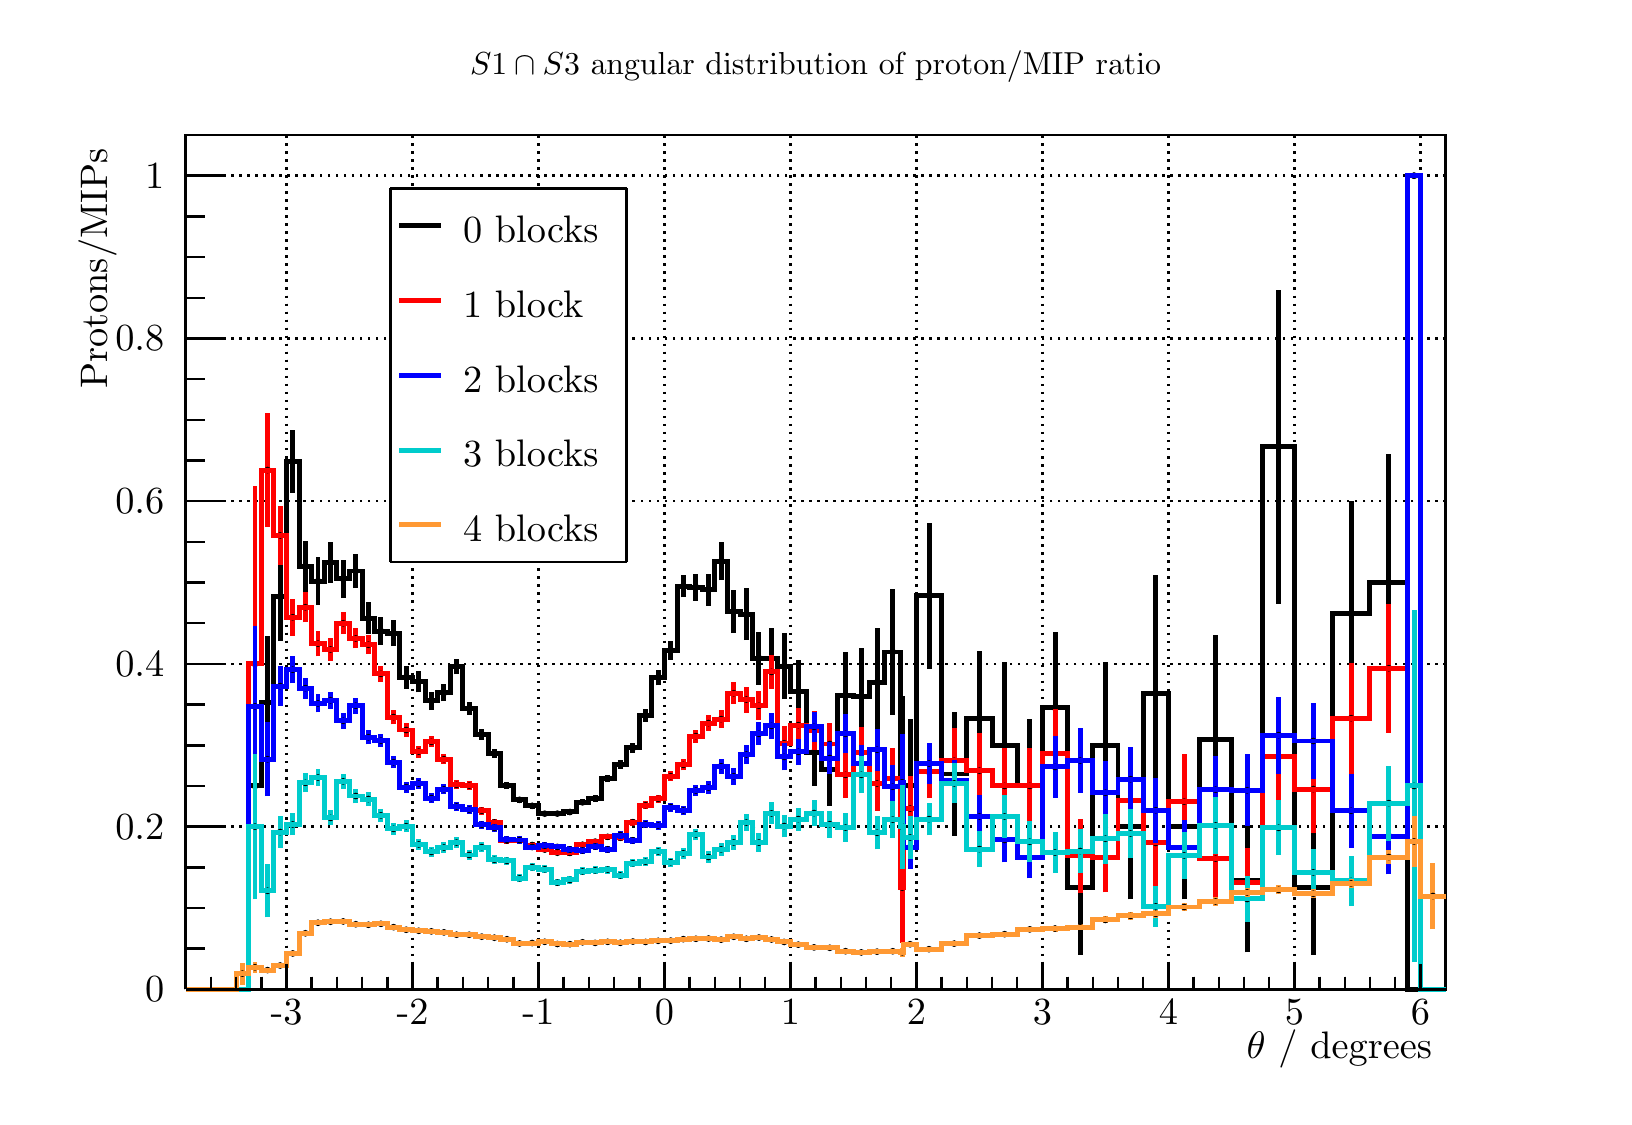
\begin{tikzpicture}
\pgfdeclareplotmark{cross} {
\pgfpathmoveto{\pgfpoint{-0.3\pgfplotmarksize}{\pgfplotmarksize}}
\pgfpathlineto{\pgfpoint{+0.3\pgfplotmarksize}{\pgfplotmarksize}}
\pgfpathlineto{\pgfpoint{+0.3\pgfplotmarksize}{0.3\pgfplotmarksize}}
\pgfpathlineto{\pgfpoint{+1\pgfplotmarksize}{0.3\pgfplotmarksize}}
\pgfpathlineto{\pgfpoint{+1\pgfplotmarksize}{-0.3\pgfplotmarksize}}
\pgfpathlineto{\pgfpoint{+0.3\pgfplotmarksize}{-0.3\pgfplotmarksize}}
\pgfpathlineto{\pgfpoint{+0.3\pgfplotmarksize}{-1.\pgfplotmarksize}}
\pgfpathlineto{\pgfpoint{-0.3\pgfplotmarksize}{-1.\pgfplotmarksize}}
\pgfpathlineto{\pgfpoint{-0.3\pgfplotmarksize}{-0.3\pgfplotmarksize}}
\pgfpathlineto{\pgfpoint{-1.\pgfplotmarksize}{-0.3\pgfplotmarksize}}
\pgfpathlineto{\pgfpoint{-1.\pgfplotmarksize}{0.3\pgfplotmarksize}}
\pgfpathlineto{\pgfpoint{-0.3\pgfplotmarksize}{0.3\pgfplotmarksize}}
\pgfpathclose
\pgfusepathqstroke
}
\pgfdeclareplotmark{cross*} {
\pgfpathmoveto{\pgfpoint{-0.3\pgfplotmarksize}{\pgfplotmarksize}}
\pgfpathlineto{\pgfpoint{+0.3\pgfplotmarksize}{\pgfplotmarksize}}
\pgfpathlineto{\pgfpoint{+0.3\pgfplotmarksize}{0.3\pgfplotmarksize}}
\pgfpathlineto{\pgfpoint{+1\pgfplotmarksize}{0.3\pgfplotmarksize}}
\pgfpathlineto{\pgfpoint{+1\pgfplotmarksize}{-0.3\pgfplotmarksize}}
\pgfpathlineto{\pgfpoint{+0.3\pgfplotmarksize}{-0.3\pgfplotmarksize}}
\pgfpathlineto{\pgfpoint{+0.3\pgfplotmarksize}{-1.\pgfplotmarksize}}
\pgfpathlineto{\pgfpoint{-0.3\pgfplotmarksize}{-1.\pgfplotmarksize}}
\pgfpathlineto{\pgfpoint{-0.3\pgfplotmarksize}{-0.3\pgfplotmarksize}}
\pgfpathlineto{\pgfpoint{-1.\pgfplotmarksize}{-0.3\pgfplotmarksize}}
\pgfpathlineto{\pgfpoint{-1.\pgfplotmarksize}{0.3\pgfplotmarksize}}
\pgfpathlineto{\pgfpoint{-0.3\pgfplotmarksize}{0.3\pgfplotmarksize}}
\pgfpathclose
\pgfusepathqfillstroke
}
\pgfdeclareplotmark{newstar} {
\pgfpathmoveto{\pgfqpoint{0pt}{\pgfplotmarksize}}
\pgfpathlineto{\pgfqpointpolar{44}{0.5\pgfplotmarksize}}
\pgfpathlineto{\pgfqpointpolar{18}{\pgfplotmarksize}}
\pgfpathlineto{\pgfqpointpolar{-20}{0.5\pgfplotmarksize}}
\pgfpathlineto{\pgfqpointpolar{-54}{\pgfplotmarksize}}
\pgfpathlineto{\pgfqpointpolar{-90}{0.5\pgfplotmarksize}}
\pgfpathlineto{\pgfqpointpolar{234}{\pgfplotmarksize}}
\pgfpathlineto{\pgfqpointpolar{198}{0.5\pgfplotmarksize}}
\pgfpathlineto{\pgfqpointpolar{162}{\pgfplotmarksize}}
\pgfpathlineto{\pgfqpointpolar{134}{0.5\pgfplotmarksize}}
\pgfpathclose
\pgfusepathqstroke
}
\pgfdeclareplotmark{newstar*} {
\pgfpathmoveto{\pgfqpoint{0pt}{\pgfplotmarksize}}
\pgfpathlineto{\pgfqpointpolar{44}{0.5\pgfplotmarksize}}
\pgfpathlineto{\pgfqpointpolar{18}{\pgfplotmarksize}}
\pgfpathlineto{\pgfqpointpolar{-20}{0.5\pgfplotmarksize}}
\pgfpathlineto{\pgfqpointpolar{-54}{\pgfplotmarksize}}
\pgfpathlineto{\pgfqpointpolar{-90}{0.5\pgfplotmarksize}}
\pgfpathlineto{\pgfqpointpolar{234}{\pgfplotmarksize}}
\pgfpathlineto{\pgfqpointpolar{198}{0.5\pgfplotmarksize}}
\pgfpathlineto{\pgfqpointpolar{162}{\pgfplotmarksize}}
\pgfpathlineto{\pgfqpointpolar{134}{0.5\pgfplotmarksize}}
\pgfpathclose
\pgfusepathqfillstroke
}
\definecolor{c}{rgb}{1,1,1};
\draw [color=c, fill=c] (0,0) rectangle (20,13.5632);
\draw [color=c, fill=c] (2,1.35632) rectangle (18,12.2069);
\definecolor{c}{rgb}{0,0,0};
\draw [c,line width=0.9] (2,1.35632) -- (2,12.2069) -- (18,12.2069) -- (18,1.35632) -- (2,1.35632);
\definecolor{c}{rgb}{1,1,1};
\draw [color=c, fill=c] (2,1.35632) rectangle (18,12.2069);
\definecolor{c}{rgb}{0,0,0};
\draw [c,line width=0.9] (2,1.35632) -- (2,12.2069) -- (18,12.2069) -- (18,1.35632) -- (2,1.35632);
\draw [c,line width=0.9] (2,1.35632) -- (18,1.35632);
\draw [c,dotted,line width=0.9] (3.28,12.2069) -- (3.28,1.35632);
\draw [c,dotted,line width=0.9] (4.88,12.2069) -- (4.88,1.35632);
\draw [c,dotted,line width=0.9] (6.48,12.2069) -- (6.48,1.35632);
\draw [c,dotted,line width=0.9] (8.08,12.2069) -- (8.08,1.35632);
\draw [c,dotted,line width=0.9] (9.68,12.2069) -- (9.68,1.35632);
\draw [c,dotted,line width=0.9] (11.28,12.2069) -- (11.28,1.35632);
\draw [c,dotted,line width=0.9] (12.88,12.2069) -- (12.88,1.35632);
\draw [c,dotted,line width=0.9] (14.48,12.2069) -- (14.48,1.35632);
\draw [c,dotted,line width=0.9] (16.08,12.2069) -- (16.08,1.35632);
\draw [c,dotted,line width=0.9] (17.68,12.2069) -- (17.68,1.35632);
\draw [c,dotted,line width=0.9] (3.28,12.2069) -- (3.28,1.35632);
\draw [c,dotted,line width=0.9] (17.68,12.2069) -- (17.68,1.35632);
\draw [c,line width=0.9] (2,1.35632) -- (2,12.2069);
\draw [c,dotted,line width=0.9] (18,1.35632) -- (2,1.35632);
\draw [c,dotted,line width=0.9] (18,3.4231) -- (2,3.4231);
\draw [c,dotted,line width=0.9] (18,5.48987) -- (2,5.48987);
\draw [c,dotted,line width=0.9] (18,7.55665) -- (2,7.55665);
\draw [c,dotted,line width=0.9] (18,9.62343) -- (2,9.62343);
\draw [c,dotted,line width=0.9] (18,11.6902) -- (2,11.6902);
\draw [c,dotted,line width=0.9] (18,11.6902) -- (2,11.6902);
\definecolor{c}{rgb}{0,0,0.6};
\draw [c,line width=0.9] (2,1.35632) -- (2.16,1.35632) -- (2.16,1.35632) -- (2.32,1.35632) -- (2.32,1.35632) -- (2.48,1.35632) -- (2.48,1.35632) -- (2.64,1.35632) -- (2.64,1.35632) -- (2.8,1.35632) -- (2.8,1.35632) -- (2.96,1.35632) -- (2.96,1.35632)
 -- (3.12,1.35632) -- (3.12,1.35632) -- (3.28,1.35632) -- (3.28,1.35632) -- (3.44,1.35632) -- (3.44,1.35632) -- (3.6,1.35632) -- (3.6,1.35632) -- (3.76,1.35632) -- (3.76,1.35632) -- (3.92,1.35632) -- (3.92,1.35632) -- (4.08,1.35632) -- (4.08,1.35632)
 -- (4.24,1.35632) -- (4.24,1.35632) -- (4.4,1.35632) -- (4.4,1.35632) -- (4.56,1.35632) -- (4.56,1.35632) -- (4.72,1.35632) -- (4.72,1.35632) -- (4.88,1.35632) -- (4.88,1.35632) -- (5.04,1.35632) -- (5.04,1.35632) -- (5.2,1.35632) -- (5.2,1.35632)
 -- (5.36,1.35632) -- (5.36,1.35632) -- (5.52,1.35632) -- (5.52,1.35632) -- (5.68,1.35632) -- (5.68,1.35632) -- (5.84,1.35632) -- (5.84,1.35632) -- (6,1.35632) -- (6,1.35632) -- (6.16,1.35632) -- (6.16,1.35632) -- (6.32,1.35632) -- (6.32,1.35632) --
 (6.48,1.35632) -- (6.48,1.35632) -- (6.64,1.35632) -- (6.64,1.35632) -- (6.8,1.35632) -- (6.8,1.35632) -- (6.96,1.35632) -- (6.96,1.35632) -- (7.12,1.35632) -- (7.12,1.35632) -- (7.28,1.35632) -- (7.28,1.35632) -- (7.44,1.35632) -- (7.44,1.35632) --
 (7.6,1.35632) -- (7.6,1.35632) -- (7.76,1.35632) -- (7.76,1.35632) -- (7.92,1.35632) -- (7.92,1.35632) -- (8.08,1.35632) -- (8.08,1.35632) -- (8.24,1.35632) -- (8.24,1.35632) -- (8.4,1.35632) -- (8.4,1.35632) -- (8.56,1.35632) -- (8.56,1.35632) --
 (8.72,1.35632) -- (8.72,1.35632) -- (8.88,1.35632) -- (8.88,1.35632) -- (9.04,1.35632) -- (9.04,1.35632) -- (9.2,1.35632) -- (9.2,1.35632) -- (9.36,1.35632) -- (9.36,1.35632) -- (9.52,1.35632) -- (9.52,1.35632) -- (9.68,1.35632) -- (9.68,1.35632) --
 (9.88,1.35632) -- (9.88,1.35632) -- (10.08,1.35632) -- (10.08,1.35632) -- (10.28,1.35632) -- (10.28,1.35632) -- (10.48,1.35632) -- (10.48,1.35632) -- (10.68,1.35632) -- (10.68,1.35632) -- (10.88,1.35632) -- (10.88,1.35632) -- (11.08,1.35632) --
 (11.08,1.35632) -- (11.12,1.35632) -- (11.12,1.35632) -- (11.28,1.35632) -- (11.28,1.35632) -- (11.6,1.35632) -- (11.6,1.35632) -- (11.92,1.35632) -- (11.92,1.35632) -- (12.24,1.35632) -- (12.24,1.35632) -- (12.56,1.35632) -- (12.56,1.35632) --
 (12.88,1.35632) -- (12.88,1.35632) -- (13.2,1.35632) -- (13.2,1.35632) -- (13.52,1.35632) -- (13.52,1.35632) -- (13.84,1.35632) -- (13.84,1.35632) -- (14.16,1.35632) -- (14.16,1.35632) -- (14.48,1.35632) -- (14.48,1.35632) -- (14.88,1.35632) --
 (14.88,1.35632) -- (15.28,1.35632) -- (15.28,1.35632) -- (15.68,1.35632) -- (15.68,1.35632) -- (16.08,1.35632) -- (16.08,1.35632) -- (16.56,1.35632) -- (16.56,1.35632) -- (17.04,1.35632) -- (17.04,1.35632) -- (17.52,1.35632) -- (17.52,1.35632) --
 (17.68,1.35632) -- (17.68,1.35632) -- (18,1.35632);
\definecolor{c}{rgb}{0,0,0};
\draw [c,line width=0.9] (2,1.35632) -- (18,1.35632);
\draw [anchor= east] (18,0.596782) node[scale=1.38496, color=c, rotate=0]{$ \theta$ / degrees};
\draw [c,line width=0.9] (3.28,1.68184) -- (3.28,1.35632);
\draw [c,line width=0.9] (3.6,1.51908) -- (3.6,1.35632);
\draw [c,line width=0.9] (3.92,1.51908) -- (3.92,1.35632);
\draw [c,line width=0.9] (4.24,1.51908) -- (4.24,1.35632);
\draw [c,line width=0.9] (4.56,1.51908) -- (4.56,1.35632);
\draw [c,line width=0.9] (4.88,1.68184) -- (4.88,1.35632);
\draw [c,line width=0.9] (5.2,1.51908) -- (5.2,1.35632);
\draw [c,line width=0.9] (5.52,1.51908) -- (5.52,1.35632);
\draw [c,line width=0.9] (5.84,1.51908) -- (5.84,1.35632);
\draw [c,line width=0.9] (6.16,1.51908) -- (6.16,1.35632);
\draw [c,line width=0.9] (6.48,1.68184) -- (6.48,1.35632);
\draw [c,line width=0.9] (6.8,1.51908) -- (6.8,1.35632);
\draw [c,line width=0.9] (7.12,1.51908) -- (7.12,1.35632);
\draw [c,line width=0.9] (7.44,1.51908) -- (7.44,1.35632);
\draw [c,line width=0.9] (7.76,1.51908) -- (7.76,1.35632);
\draw [c,line width=0.9] (8.08,1.68184) -- (8.08,1.35632);
\draw [c,line width=0.9] (8.4,1.51908) -- (8.4,1.35632);
\draw [c,line width=0.9] (8.72,1.51908) -- (8.72,1.35632);
\draw [c,line width=0.9] (9.04,1.51908) -- (9.04,1.35632);
\draw [c,line width=0.9] (9.36,1.51908) -- (9.36,1.35632);
\draw [c,line width=0.9] (9.68,1.68184) -- (9.68,1.35632);
\draw [c,line width=0.9] (10,1.51908) -- (10,1.35632);
\draw [c,line width=0.9] (10.32,1.51908) -- (10.32,1.35632);
\draw [c,line width=0.9] (10.64,1.51908) -- (10.64,1.35632);
\draw [c,line width=0.9] (10.96,1.51908) -- (10.96,1.35632);
\draw [c,line width=0.9] (11.28,1.68184) -- (11.28,1.35632);
\draw [c,line width=0.9] (11.6,1.51908) -- (11.6,1.35632);
\draw [c,line width=0.9] (11.92,1.51908) -- (11.92,1.35632);
\draw [c,line width=0.9] (12.24,1.51908) -- (12.24,1.35632);
\draw [c,line width=0.9] (12.56,1.51908) -- (12.56,1.35632);
\draw [c,line width=0.9] (12.88,1.68184) -- (12.88,1.35632);
\draw [c,line width=0.9] (13.2,1.51908) -- (13.2,1.35632);
\draw [c,line width=0.9] (13.52,1.51908) -- (13.52,1.35632);
\draw [c,line width=0.9] (13.84,1.51908) -- (13.84,1.35632);
\draw [c,line width=0.9] (14.16,1.51908) -- (14.16,1.35632);
\draw [c,line width=0.9] (14.48,1.68184) -- (14.48,1.35632);
\draw [c,line width=0.9] (14.8,1.51908) -- (14.8,1.35632);
\draw [c,line width=0.9] (15.12,1.51908) -- (15.12,1.35632);
\draw [c,line width=0.9] (15.44,1.51908) -- (15.44,1.35632);
\draw [c,line width=0.9] (15.76,1.51908) -- (15.76,1.35632);
\draw [c,line width=0.9] (16.08,1.68184) -- (16.08,1.35632);
\draw [c,line width=0.9] (16.4,1.51908) -- (16.4,1.35632);
\draw [c,line width=0.9] (16.72,1.51908) -- (16.72,1.35632);
\draw [c,line width=0.9] (17.04,1.51908) -- (17.04,1.35632);
\draw [c,line width=0.9] (17.36,1.51908) -- (17.36,1.35632);
\draw [c,line width=0.9] (17.68,1.68184) -- (17.68,1.35632);
\draw [c,line width=0.9] (3.28,1.68184) -- (3.28,1.35632);
\draw [c,line width=0.9] (2.96,1.51908) -- (2.96,1.35632);
\draw [c,line width=0.9] (2.64,1.51908) -- (2.64,1.35632);
\draw [c,line width=0.9] (2.32,1.51908) -- (2.32,1.35632);
\draw [c,line width=0.9] (17.68,1.68184) -- (17.68,1.35632);
\draw [anchor=base] (3.28,0.908736) node[scale=1.38496, color=c, rotate=0]{-3};
\draw [anchor=base] (4.88,0.908736) node[scale=1.38496, color=c, rotate=0]{-2};
\draw [anchor=base] (6.48,0.908736) node[scale=1.38496, color=c, rotate=0]{-1};
\draw [anchor=base] (8.08,0.908736) node[scale=1.38496, color=c, rotate=0]{0};
\draw [anchor=base] (9.68,0.908736) node[scale=1.38496, color=c, rotate=0]{1};
\draw [anchor=base] (11.28,0.908736) node[scale=1.38496, color=c, rotate=0]{2};
\draw [anchor=base] (12.88,0.908736) node[scale=1.38496, color=c, rotate=0]{3};
\draw [anchor=base] (14.48,0.908736) node[scale=1.38496, color=c, rotate=0]{4};
\draw [anchor=base] (16.08,0.908736) node[scale=1.38496, color=c, rotate=0]{5};
\draw [anchor=base] (17.68,0.908736) node[scale=1.38496, color=c, rotate=0]{6};
\draw [c,line width=0.9] (2,1.35632) -- (2,12.2069);
\draw [anchor= east] (0.88,12.2069) node[scale=1.38496, color=c, rotate=90]{  Protons/MIPs};
\draw [c,line width=0.9] (2.48,1.35632) -- (2,1.35632);
\draw [c,line width=0.9] (2.24,1.87302) -- (2,1.87302);
\draw [c,line width=0.9] (2.24,2.38971) -- (2,2.38971);
\draw [c,line width=0.9] (2.24,2.9064) -- (2,2.9064);
\draw [c,line width=0.9] (2.48,3.4231) -- (2,3.4231);
\draw [c,line width=0.9] (2.24,3.93979) -- (2,3.93979);
\draw [c,line width=0.9] (2.24,4.45649) -- (2,4.45649);
\draw [c,line width=0.9] (2.24,4.97318) -- (2,4.97318);
\draw [c,line width=0.9] (2.48,5.48987) -- (2,5.48987);
\draw [c,line width=0.9] (2.24,6.00657) -- (2,6.00657);
\draw [c,line width=0.9] (2.24,6.52326) -- (2,6.52326);
\draw [c,line width=0.9] (2.24,7.03996) -- (2,7.03996);
\draw [c,line width=0.9] (2.48,7.55665) -- (2,7.55665);
\draw [c,line width=0.9] (2.24,8.07334) -- (2,8.07334);
\draw [c,line width=0.9] (2.24,8.59004) -- (2,8.59004);
\draw [c,line width=0.9] (2.24,9.10673) -- (2,9.10673);
\draw [c,line width=0.9] (2.48,9.62343) -- (2,9.62343);
\draw [c,line width=0.9] (2.24,10.1401) -- (2,10.1401);
\draw [c,line width=0.9] (2.24,10.6568) -- (2,10.6568);
\draw [c,line width=0.9] (2.24,11.1735) -- (2,11.1735);
\draw [c,line width=0.9] (2.48,11.6902) -- (2,11.6902);
\draw [c,line width=0.9] (2.48,11.6902) -- (2,11.6902);
\draw [anchor= east] (1.9,1.35632) node[scale=1.38496, color=c, rotate=0]{0};
\draw [anchor= east] (1.9,3.4231) node[scale=1.38496, color=c, rotate=0]{0.2};
\draw [anchor= east] (1.9,5.48987) node[scale=1.38496, color=c, rotate=0]{0.4};
\draw [anchor= east] (1.9,7.55665) node[scale=1.38496, color=c, rotate=0]{0.6};
\draw [anchor= east] (1.9,9.62343) node[scale=1.38496, color=c, rotate=0]{0.8};
\draw [anchor= east] (1.9,11.6902) node[scale=1.38496, color=c, rotate=0]{1};
\draw [c,line width=1.8] (2.88,2.82112) -- (2.88,3.93979);
\draw [c,line width=1.8] (2.88,3.93979) -- (2.88,5.05847);
\foreach \P in {(2.88,3.93979)}{\draw[mark options={color=c,fill=c},mark size=2.402402pt,mark=*,mark size=1pt] plot coordinates {\P};}
\draw [c,line width=1.8] (3.04,4.15664) -- (3.04,5.00357);
\draw [c,line width=1.8] (3.04,5.00357) -- (3.04,5.8505);
\foreach \P in {(3.04,5.00357)}{\draw[mark options={color=c,fill=c},mark size=2.402402pt,mark=*,mark size=1pt] plot coordinates {\P};}
\draw [c,line width=1.8] (3.2,5.78082) -- (3.2,6.3409);
\draw [c,line width=1.8] (3.2,6.3409) -- (3.2,6.90098);
\foreach \P in {(3.2,6.3409)}{\draw[mark options={color=c,fill=c},mark size=2.402402pt,mark=*,mark size=1pt] plot coordinates {\P};}
\draw [c,line width=1.8] (3.36,7.66171) -- (3.36,8.06308);
\draw [c,line width=1.8] (3.36,8.06308) -- (3.36,8.46445);
\foreach \P in {(3.36,8.06308)}{\draw[mark options={color=c,fill=c},mark size=2.402402pt,mark=*,mark size=1pt] plot coordinates {\P};}
\draw [c,line width=1.8] (3.52,6.40342) -- (3.52,6.72994);
\draw [c,line width=1.8] (3.52,6.72994) -- (3.52,7.05646);
\foreach \P in {(3.52,6.72994)}{\draw[mark options={color=c,fill=c},mark size=2.402402pt,mark=*,mark size=1pt] plot coordinates {\P};}
\draw [c,line width=1.8] (3.68,6.23995) -- (3.68,6.54078);
\draw [c,line width=1.8] (3.68,6.54078) -- (3.68,6.84161);
\foreach \P in {(3.68,6.54078)}{\draw[mark options={color=c,fill=c},mark size=2.402402pt,mark=*,mark size=1pt] plot coordinates {\P};}
\draw [c,line width=1.8] (3.84,6.5146) -- (3.84,6.77694);
\draw [c,line width=1.8] (3.84,6.77694) -- (3.84,7.03927);
\foreach \P in {(3.84,6.77694)}{\draw[mark options={color=c,fill=c},mark size=2.402402pt,mark=*,mark size=1pt] plot coordinates {\P};}
\draw [c,line width=1.8] (4,6.3263) -- (4,6.56879);
\draw [c,line width=1.8] (4,6.56879) -- (4,6.81127);
\foreach \P in {(4,6.56879)}{\draw[mark options={color=c,fill=c},mark size=2.402402pt,mark=*,mark size=1pt] plot coordinates {\P};}
\draw [c,line width=1.8] (4.16,6.45236) -- (4.16,6.66984);
\draw [c,line width=1.8] (4.16,6.66984) -- (4.16,6.88732);
\foreach \P in {(4.16,6.66984)}{\draw[mark options={color=c,fill=c},mark size=2.402402pt,mark=*,mark size=1pt] plot coordinates {\P};}
\draw [c,line width=1.8] (4.32,5.87082) -- (4.32,6.07224);
\draw [c,line width=1.8] (4.32,6.07224) -- (4.32,6.27367);
\foreach \P in {(4.32,6.07224)}{\draw[mark options={color=c,fill=c},mark size=2.402402pt,mark=*,mark size=1pt] plot coordinates {\P};}
\draw [c,line width=1.8] (4.48,5.72805) -- (4.48,5.90622);
\draw [c,line width=1.8] (4.48,5.90622) -- (4.48,6.08439);
\foreach \P in {(4.48,5.90622)}{\draw[mark options={color=c,fill=c},mark size=2.402402pt,mark=*,mark size=1pt] plot coordinates {\P};}
\draw [c,line width=1.8] (4.64,5.71626) -- (4.64,5.88003);
\draw [c,line width=1.8] (4.64,5.88003) -- (4.64,6.0438);
\foreach \P in {(4.64,5.88003)}{\draw[mark options={color=c,fill=c},mark size=2.402402pt,mark=*,mark size=1pt] plot coordinates {\P};}
\draw [c,line width=1.8] (4.8,5.17503) -- (4.8,5.32144);
\draw [c,line width=1.8] (4.8,5.32144) -- (4.8,5.46786);
\foreach \P in {(4.8,5.32144)}{\draw[mark options={color=c,fill=c},mark size=2.402402pt,mark=*,mark size=1pt] plot coordinates {\P};}
\draw [c,line width=1.8] (4.96,5.12903) -- (4.96,5.26285);
\draw [c,line width=1.8] (4.96,5.26285) -- (4.96,5.39668);
\foreach \P in {(4.96,5.26285)}{\draw[mark options={color=c,fill=c},mark size=2.402402pt,mark=*,mark size=1pt] plot coordinates {\P};}
\draw [c,line width=1.8] (5.12,4.90259) -- (5.12,5.02053);
\draw [c,line width=1.8] (5.12,5.02053) -- (5.12,5.13847);
\foreach \P in {(5.12,5.02053)}{\draw[mark options={color=c,fill=c},mark size=2.402402pt,mark=*,mark size=1pt] plot coordinates {\P};}
\draw [c,line width=1.8] (5.28,5.01499) -- (5.28,5.12243);
\draw [c,line width=1.8] (5.28,5.12243) -- (5.28,5.22986);
\foreach \P in {(5.28,5.12243)}{\draw[mark options={color=c,fill=c},mark size=2.402402pt,mark=*,mark size=1pt] plot coordinates {\P};}
\draw [c,line width=1.8] (5.44,5.35678) -- (5.44,5.45532);
\draw [c,line width=1.8] (5.44,5.45532) -- (5.44,5.55386);
\foreach \P in {(5.44,5.45532)}{\draw[mark options={color=c,fill=c},mark size=2.402402pt,mark=*,mark size=1pt] plot coordinates {\P};}
\draw [c,line width=1.8] (5.6,4.84175) -- (5.6,4.92626);
\draw [c,line width=1.8] (5.6,4.92626) -- (5.6,5.01077);
\foreach \P in {(5.6,4.92626)}{\draw[mark options={color=c,fill=c},mark size=2.402402pt,mark=*,mark size=1pt] plot coordinates {\P};}
\draw [c,line width=1.8] (5.76,4.52635) -- (5.76,4.59642);
\draw [c,line width=1.8] (5.76,4.59642) -- (5.76,4.66648);
\foreach \P in {(5.76,4.59642)}{\draw[mark options={color=c,fill=c},mark size=2.402402pt,mark=*,mark size=1pt] plot coordinates {\P};}
\draw [c,line width=1.8] (5.92,4.29619) -- (5.92,4.35491);
\draw [c,line width=1.8] (5.92,4.35491) -- (5.92,4.41363);
\foreach \P in {(5.92,4.35491)}{\draw[mark options={color=c,fill=c},mark size=2.402402pt,mark=*,mark size=1pt] plot coordinates {\P};}
\draw [c,line width=1.8] (6.08,3.89665) -- (6.08,3.94452);
\draw [c,line width=1.8] (6.08,3.94452) -- (6.08,3.99239);
\foreach \P in {(6.08,3.94452)}{\draw[mark options={color=c,fill=c},mark size=2.402402pt,mark=*,mark size=1pt] plot coordinates {\P};}
\draw [c,line width=1.8] (6.24,3.72359) -- (6.24,3.7641);
\draw [c,line width=1.8] (6.24,3.7641) -- (6.24,3.8046);
\foreach \P in {(6.24,3.7641)}{\draw[mark options={color=c,fill=c},mark size=2.402402pt,mark=*,mark size=1pt] plot coordinates {\P};}
\draw [c,line width=1.8] (6.4,3.65134) -- (6.4,3.68776);
\draw [c,line width=1.8] (6.4,3.68776) -- (6.4,3.72419);
\foreach \P in {(6.4,3.68776)}{\draw[mark options={color=c,fill=c},mark size=2.402402pt,mark=*,mark size=1pt] plot coordinates {\P};}
\draw [c,line width=1.8] (6.56,3.55409) -- (6.56,3.58784);
\draw [c,line width=1.8] (6.56,3.58784) -- (6.56,3.62159);
\foreach \P in {(6.56,3.58784)}{\draw[mark options={color=c,fill=c},mark size=2.402402pt,mark=*,mark size=1pt] plot coordinates {\P};}
\draw [c,line width=1.8] (6.72,3.55518) -- (6.72,3.58863);
\draw [c,line width=1.8] (6.72,3.58863) -- (6.72,3.62209);
\foreach \P in {(6.72,3.58863)}{\draw[mark options={color=c,fill=c},mark size=2.402402pt,mark=*,mark size=1pt] plot coordinates {\P};}
\draw [c,line width=1.8] (6.88,3.57488) -- (6.88,3.60946);
\draw [c,line width=1.8] (6.88,3.60946) -- (6.88,3.64404);
\foreach \P in {(6.88,3.60946)}{\draw[mark options={color=c,fill=c},mark size=2.402402pt,mark=*,mark size=1pt] plot coordinates {\P};}
\draw [c,line width=1.8] (7.04,3.69352) -- (7.04,3.73153);
\draw [c,line width=1.8] (7.04,3.73153) -- (7.04,3.76953);
\foreach \P in {(7.04,3.73153)}{\draw[mark options={color=c,fill=c},mark size=2.402402pt,mark=*,mark size=1pt] plot coordinates {\P};}
\draw [c,line width=1.8] (7.2,3.74045) -- (7.2,3.78255);
\draw [c,line width=1.8] (7.2,3.78255) -- (7.2,3.82464);
\foreach \P in {(7.2,3.78255)}{\draw[mark options={color=c,fill=c},mark size=2.402402pt,mark=*,mark size=1pt] plot coordinates {\P};}
\draw [c,line width=1.8] (7.36,3.98624) -- (7.36,4.03499);
\draw [c,line width=1.8] (7.36,4.03499) -- (7.36,4.08373);
\foreach \P in {(7.36,4.03499)}{\draw[mark options={color=c,fill=c},mark size=2.402402pt,mark=*,mark size=1pt] plot coordinates {\P};}
\draw [c,line width=1.8] (7.52,4.15815) -- (7.52,4.2143);
\draw [c,line width=1.8] (7.52,4.2143) -- (7.52,4.27046);
\foreach \P in {(7.52,4.2143)}{\draw[mark options={color=c,fill=c},mark size=2.402402pt,mark=*,mark size=1pt] plot coordinates {\P};}
\draw [c,line width=1.8] (7.68,4.3576) -- (7.68,4.42369);
\draw [c,line width=1.8] (7.68,4.42369) -- (7.68,4.48977);
\foreach \P in {(7.68,4.42369)}{\draw[mark options={color=c,fill=c},mark size=2.402402pt,mark=*,mark size=1pt] plot coordinates {\P};}
\draw [c,line width=1.8] (7.84,4.75402) -- (7.84,4.83531);
\draw [c,line width=1.8] (7.84,4.83531) -- (7.84,4.9166);
\foreach \P in {(7.84,4.83531)}{\draw[mark options={color=c,fill=c},mark size=2.402402pt,mark=*,mark size=1pt] plot coordinates {\P};}
\draw [c,line width=1.8] (8,5.21746) -- (8,5.31813);
\draw [c,line width=1.8] (8,5.31813) -- (8,5.4188);
\foreach \P in {(8,5.31813)}{\draw[mark options={color=c,fill=c},mark size=2.402402pt,mark=*,mark size=1pt] plot coordinates {\P};}
\draw [c,line width=1.8] (8.16,5.5424) -- (8.16,5.66458);
\draw [c,line width=1.8] (8.16,5.66458) -- (8.16,5.78676);
\foreach \P in {(8.16,5.66458)}{\draw[mark options={color=c,fill=c},mark size=2.402402pt,mark=*,mark size=1pt] plot coordinates {\P};}
\draw [c,line width=1.8] (8.32,6.33453) -- (8.32,6.47889);
\draw [c,line width=1.8] (8.32,6.47889) -- (8.32,6.62325);
\foreach \P in {(8.32,6.47889)}{\draw[mark options={color=c,fill=c},mark size=2.402402pt,mark=*,mark size=1pt] plot coordinates {\P};}
\draw [c,line width=1.8] (8.48,6.29395) -- (8.48,6.46598);
\draw [c,line width=1.8] (8.48,6.46598) -- (8.48,6.63801);
\foreach \P in {(8.48,6.46598)}{\draw[mark options={color=c,fill=c},mark size=2.402402pt,mark=*,mark size=1pt] plot coordinates {\P};}
\draw [c,line width=1.8] (8.64,6.23171) -- (8.64,6.431);
\draw [c,line width=1.8] (8.64,6.431) -- (8.64,6.63028);
\foreach \P in {(8.64,6.431)}{\draw[mark options={color=c,fill=c},mark size=2.402402pt,mark=*,mark size=1pt] plot coordinates {\P};}
\draw [c,line width=1.8] (8.8,6.55226) -- (8.8,6.79284);
\draw [c,line width=1.8] (8.8,6.79284) -- (8.8,7.03342);
\foreach \P in {(8.8,6.79284)}{\draw[mark options={color=c,fill=c},mark size=2.402402pt,mark=*,mark size=1pt] plot coordinates {\P};}
\draw [c,line width=1.8] (8.96,5.88016) -- (8.96,6.15525);
\draw [c,line width=1.8] (8.96,6.15525) -- (8.96,6.43034);
\foreach \P in {(8.96,6.15525)}{\draw[mark options={color=c,fill=c},mark size=2.402402pt,mark=*,mark size=1pt] plot coordinates {\P};}
\draw [c,line width=1.8] (9.12,5.79345) -- (9.12,6.12256);
\draw [c,line width=1.8] (9.12,6.12256) -- (9.12,6.45167);
\foreach \P in {(9.12,6.12256)}{\draw[mark options={color=c,fill=c},mark size=2.402402pt,mark=*,mark size=1pt] plot coordinates {\P};}
\draw [c,line width=1.8] (9.28,5.22532) -- (9.28,5.56303);
\draw [c,line width=1.8] (9.28,5.56303) -- (9.28,5.90075);
\foreach \P in {(9.28,5.56303)}{\draw[mark options={color=c,fill=c},mark size=2.402402pt,mark=*,mark size=1pt] plot coordinates {\P};}
\draw [c,line width=1.8] (9.44,5.17837) -- (9.44,5.55993);
\draw [c,line width=1.8] (9.44,5.55993) -- (9.44,5.9415);
\foreach \P in {(9.44,5.55993)}{\draw[mark options={color=c,fill=c},mark size=2.402402pt,mark=*,mark size=1pt] plot coordinates {\P};}
\draw [c,line width=1.8] (9.6,5.04307) -- (9.6,5.46156);
\draw [c,line width=1.8] (9.6,5.46156) -- (9.6,5.88006);
\foreach \P in {(9.6,5.46156)}{\draw[mark options={color=c,fill=c},mark size=2.402402pt,mark=*,mark size=1pt] plot coordinates {\P};}
\draw [c,line width=1.8] (9.78,4.73621) -- (9.78,5.13866);
\draw [c,line width=1.8] (9.78,5.13866) -- (9.78,5.5411);
\foreach \P in {(9.78,5.13866)}{\draw[mark options={color=c,fill=c},mark size=2.402402pt,mark=*,mark size=1pt] plot coordinates {\P};}
\draw [c,line width=1.8] (9.98,3.94159) -- (9.98,4.37037);
\draw [c,line width=1.8] (9.98,4.37037) -- (9.98,4.79915);
\foreach \P in {(9.98,4.37037)}{\draw[mark options={color=c,fill=c},mark size=2.402402pt,mark=*,mark size=1pt] plot coordinates {\P};}
\draw [c,line width=1.8] (10.18,3.68769) -- (10.18,4.14647);
\draw [c,line width=1.8] (10.18,4.14647) -- (10.18,4.60525);
\foreach \P in {(10.18,4.14647)}{\draw[mark options={color=c,fill=c},mark size=2.402402pt,mark=*,mark size=1pt] plot coordinates {\P};}
\draw [c,line width=1.8] (10.38,4.54652) -- (10.38,5.09146);
\draw [c,line width=1.8] (10.38,5.09146) -- (10.38,5.63639);
\foreach \P in {(10.38,5.09146)}{\draw[mark options={color=c,fill=c},mark size=2.402402pt,mark=*,mark size=1pt] plot coordinates {\P};}
\draw [c,line width=1.8] (10.58,4.45026) -- (10.58,5.07006);
\draw [c,line width=1.8] (10.58,5.07006) -- (10.58,5.68986);
\foreach \P in {(10.58,5.07006)}{\draw[mark options={color=c,fill=c},mark size=2.402402pt,mark=*,mark size=1pt] plot coordinates {\P};}
\draw [c,line width=1.8] (10.78,4.56785) -- (10.78,5.2559);
\draw [c,line width=1.8] (10.78,5.2559) -- (10.78,5.94395);
\foreach \P in {(10.78,5.2559)}{\draw[mark options={color=c,fill=c},mark size=2.402402pt,mark=*,mark size=1pt] plot coordinates {\P};}
\draw [c,line width=1.8] (10.98,4.84601) -- (10.98,5.6411);
\draw [c,line width=1.8] (10.98,5.6411) -- (10.98,6.43619);
\foreach \P in {(10.98,5.6411)}{\draw[mark options={color=c,fill=c},mark size=2.402402pt,mark=*,mark size=1pt] plot coordinates {\P};}
\draw [c,line width=1.8] (11.1,2.22067) -- (11.1,3.65274);
\draw [c,line width=1.8] (11.1,3.65274) -- (11.1,5.08481);
\foreach \P in {(11.1,3.65274)}{\draw[mark options={color=c,fill=c},mark size=2.402402pt,mark=*,mark size=1pt] plot coordinates {\P};}
\draw [c,line width=1.8] (11.2,3.09415) -- (11.2,3.93979);
\draw [c,line width=1.8] (11.2,3.93979) -- (11.2,4.78543);
\foreach \P in {(11.2,3.93979)}{\draw[mark options={color=c,fill=c},mark size=2.402402pt,mark=*,mark size=1pt] plot coordinates {\P};}
\draw [c,line width=1.8] (11.44,5.42906) -- (11.44,6.35659);
\draw [c,line width=1.8] (11.44,6.35659) -- (11.44,7.28411);
\foreach \P in {(11.44,6.35659)}{\draw[mark options={color=c,fill=c},mark size=2.402402pt,mark=*,mark size=1pt] plot coordinates {\P};}
\draw [c,line width=1.8] (11.76,3.30989) -- (11.76,4.09176);
\draw [c,line width=1.8] (11.76,4.09176) -- (11.76,4.87363);
\foreach \P in {(11.76,4.09176)}{\draw[mark options={color=c,fill=c},mark size=2.402402pt,mark=*,mark size=1pt] plot coordinates {\P};}
\draw [c,line width=1.8] (12.08,3.95294) -- (12.08,4.80095);
\draw [c,line width=1.8] (12.08,4.80095) -- (12.08,5.64896);
\foreach \P in {(12.08,4.80095)}{\draw[mark options={color=c,fill=c},mark size=2.402402pt,mark=*,mark size=1pt] plot coordinates {\P};}
\draw [c,line width=1.8] (12.4,3.39758) -- (12.4,4.45649);
\draw [c,line width=1.8] (12.4,4.45649) -- (12.4,5.51539);
\foreach \P in {(12.4,4.45649)}{\draw[mark options={color=c,fill=c},mark size=2.402402pt,mark=*,mark size=1pt] plot coordinates {\P};}
\draw [c,line width=1.8] (12.72,3.09415) -- (12.72,3.93979);
\draw [c,line width=1.8] (12.72,3.93979) -- (12.72,4.78543);
\foreach \P in {(12.72,3.93979)}{\draw[mark options={color=c,fill=c},mark size=2.402402pt,mark=*,mark size=1pt] plot coordinates {\P};}
\draw [c,line width=1.8] (13.04,3.96927) -- (13.04,4.93343);
\draw [c,line width=1.8] (13.04,4.93343) -- (13.04,5.89759);
\foreach \P in {(13.04,4.93343)}{\draw[mark options={color=c,fill=c},mark size=2.402402pt,mark=*,mark size=1pt] plot coordinates {\P};}
\draw [c,line width=1.8] (13.36,1.79365) -- (13.36,2.64806);
\draw [c,line width=1.8] (13.36,2.64806) -- (13.36,3.50246);
\foreach \P in {(13.36,2.64806)}{\draw[mark options={color=c,fill=c},mark size=2.402402pt,mark=*,mark size=1pt] plot coordinates {\P};}
\draw [c,line width=1.8] (13.68,3.39758) -- (13.68,4.45649);
\draw [c,line width=1.8] (13.68,4.45649) -- (13.68,5.51539);
\foreach \P in {(13.68,4.45649)}{\draw[mark options={color=c,fill=c},mark size=2.402402pt,mark=*,mark size=1pt] plot coordinates {\P};}
\draw [c,line width=1.8] (14,2.49881) -- (14,3.4231);
\draw [c,line width=1.8] (14,3.4231) -- (14,4.34739);
\foreach \P in {(14,3.4231)}{\draw[mark options={color=c,fill=c},mark size=2.402402pt,mark=*,mark size=1pt] plot coordinates {\P};}
\draw [c,line width=1.8] (14.32,3.61526) -- (14.32,5.1141);
\draw [c,line width=1.8] (14.32,5.1141) -- (14.32,6.61293);
\foreach \P in {(14.32,5.1141)}{\draw[mark options={color=c,fill=c},mark size=2.402402pt,mark=*,mark size=1pt] plot coordinates {\P};}
\draw [c,line width=1.8] (14.68,2.49881) -- (14.68,3.4231);
\draw [c,line width=1.8] (14.68,3.4231) -- (14.68,4.34739);
\foreach \P in {(14.68,3.4231)}{\draw[mark options={color=c,fill=c},mark size=2.402402pt,mark=*,mark size=1pt] plot coordinates {\P};}
\draw [c,line width=1.8] (15.08,3.21316) -- (15.08,4.53598);
\draw [c,line width=1.8] (15.08,4.53598) -- (15.08,5.85879);
\foreach \P in {(15.08,4.53598)}{\draw[mark options={color=c,fill=c},mark size=2.402402pt,mark=*,mark size=1pt] plot coordinates {\P};}
\draw [c,line width=1.8] (15.48,1.82716) -- (15.48,2.73417);
\draw [c,line width=1.8] (15.48,2.73417) -- (15.48,3.64119);
\foreach \P in {(15.48,2.73417)}{\draw[mark options={color=c,fill=c},mark size=2.402402pt,mark=*,mark size=1pt] plot coordinates {\P};}
\draw [c,line width=1.8] (15.88,6.25682) -- (15.88,8.24558);
\draw [c,line width=1.8] (15.88,8.24558) -- (15.88,10.2343);
\foreach \P in {(15.88,8.24558)}{\draw[mark options={color=c,fill=c},mark size=2.402402pt,mark=*,mark size=1pt] plot coordinates {\P};}
\draw [c,line width=1.8] (16.32,1.79365) -- (16.32,2.64806);
\draw [c,line width=1.8] (16.32,2.64806) -- (16.32,3.50246);
\foreach \P in {(16.32,2.64806)}{\draw[mark options={color=c,fill=c},mark size=2.402402pt,mark=*,mark size=1pt] plot coordinates {\P};}
\draw [c,line width=1.8] (16.8,4.697) -- (16.8,6.1258);
\draw [c,line width=1.8] (16.8,6.1258) -- (16.8,7.55461);
\foreach \P in {(16.8,6.1258)}{\draw[mark options={color=c,fill=c},mark size=2.402402pt,mark=*,mark size=1pt] plot coordinates {\P};}
\draw [c,line width=1.8] (17.28,4.88933) -- (17.28,6.52326);
\draw [c,line width=1.8] (17.28,6.52326) -- (17.28,8.15719);
\foreach \P in {(17.28,6.52326)}{\draw[mark options={color=c,fill=c},mark size=2.402402pt,mark=*,mark size=1pt] plot coordinates {\P};}
\draw [c,line width=1.8] (2,1.35632) -- (2.16,1.35632) -- (2.16,1.35632) -- (2.32,1.35632) -- (2.32,1.35632) -- (2.48,1.35632) -- (2.48,1.35632) -- (2.64,1.35632) -- (2.64,1.35632) -- (2.8,1.35632) -- (2.8,3.93979) -- (2.96,3.93979) -- (2.96,5.00357)
 -- (3.12,5.00357) -- (3.12,6.3409) -- (3.28,6.3409) -- (3.28,8.06308) -- (3.44,8.06308) -- (3.44,6.72994) -- (3.6,6.72994) -- (3.6,6.54078) -- (3.76,6.54078) -- (3.76,6.77694) -- (3.92,6.77694) -- (3.92,6.56879) -- (4.08,6.56879) -- (4.08,6.66984)
 -- (4.24,6.66984) -- (4.24,6.07224) -- (4.4,6.07224) -- (4.4,5.90622) -- (4.56,5.90622) -- (4.56,5.88003) -- (4.72,5.88003) -- (4.72,5.32144) -- (4.88,5.32144) -- (4.88,5.26285) -- (5.04,5.26285) -- (5.04,5.02053) -- (5.2,5.02053) -- (5.2,5.12243)
 -- (5.36,5.12243) -- (5.36,5.45532) -- (5.52,5.45532) -- (5.52,4.92626) -- (5.68,4.92626) -- (5.68,4.59642) -- (5.84,4.59642) -- (5.84,4.35491) -- (6,4.35491) -- (6,3.94452) -- (6.16,3.94452) -- (6.16,3.7641) -- (6.32,3.7641) -- (6.32,3.68776) --
 (6.48,3.68776) -- (6.48,3.58784) -- (6.64,3.58784) -- (6.64,3.58863) -- (6.8,3.58863) -- (6.8,3.60946) -- (6.96,3.60946) -- (6.96,3.73153) -- (7.12,3.73153) -- (7.12,3.78255) -- (7.28,3.78255) -- (7.28,4.03499) -- (7.44,4.03499) -- (7.44,4.2143) --
 (7.6,4.2143) -- (7.6,4.42369) -- (7.76,4.42369) -- (7.76,4.83531) -- (7.92,4.83531) -- (7.92,5.31813) -- (8.08,5.31813) -- (8.08,5.66458) -- (8.24,5.66458) -- (8.24,6.47889) -- (8.4,6.47889) -- (8.4,6.46598) -- (8.56,6.46598) -- (8.56,6.431) --
 (8.72,6.431) -- (8.72,6.79284) -- (8.88,6.79284) -- (8.88,6.15525) -- (9.04,6.15525) -- (9.04,6.12256) -- (9.2,6.12256) -- (9.2,5.56303) -- (9.36,5.56303) -- (9.36,5.55993) -- (9.52,5.55993) -- (9.52,5.46156) -- (9.68,5.46156) -- (9.68,5.13866) --
 (9.88,5.13866) -- (9.88,4.37037) -- (10.08,4.37037) -- (10.08,4.14647) -- (10.28,4.14647) -- (10.28,5.09146) -- (10.48,5.09146) -- (10.48,5.07006) -- (10.68,5.07006) -- (10.68,5.2559) -- (10.88,5.2559) -- (10.88,5.6411) -- (11.08,5.6411) --
 (11.08,3.65274) -- (11.12,3.65274) -- (11.12,3.93979) -- (11.28,3.93979) -- (11.28,6.35659) -- (11.6,6.35659) -- (11.6,4.09176) -- (11.92,4.09176) -- (11.92,4.80095) -- (12.24,4.80095) -- (12.24,4.45649) -- (12.56,4.45649) -- (12.56,3.93979) --
 (12.88,3.93979) -- (12.88,4.93343) -- (13.2,4.93343) -- (13.2,2.64806) -- (13.52,2.64806) -- (13.52,4.45649) -- (13.84,4.45649) -- (13.84,3.4231) -- (14.16,3.4231) -- (14.16,5.1141) -- (14.48,5.1141) -- (14.48,3.4231) -- (14.88,3.4231) --
 (14.88,4.53598) -- (15.28,4.53598) -- (15.28,2.73417) -- (15.68,2.73417) -- (15.68,8.24558) -- (16.08,8.24558) -- (16.08,2.64806) -- (16.56,2.64806) -- (16.56,6.1258) -- (17.04,6.1258) -- (17.04,6.52326) -- (17.52,6.52326) -- (17.52,1.35632) --
 (17.68,1.35632) -- (17.68,1.35632) -- (18,1.35632);
\definecolor{c}{rgb}{1,0,0};
\draw [c,line width=1.8] (2.88,3.22583) -- (2.88,5.48987);
\draw [c,line width=1.8] (2.88,5.48987) -- (2.88,7.75391);
\definecolor{c}{rgb}{0,0,0};
\foreach \P in {(2.88,5.48987)}{\draw[mark options={color=c,fill=c},mark size=2.402402pt,mark=*,mark size=1pt] plot coordinates {\P};}
\definecolor{c}{rgb}{1,0,0};
\draw [c,line width=1.8] (3.04,7.22814) -- (3.04,7.95242);
\draw [c,line width=1.8] (3.04,7.95242) -- (3.04,8.67669);
\definecolor{c}{rgb}{0,0,0};
\foreach \P in {(3.04,7.95242)}{\draw[mark options={color=c,fill=c},mark size=2.402402pt,mark=*,mark size=1pt] plot coordinates {\P};}
\definecolor{c}{rgb}{1,0,0};
\draw [c,line width=1.8] (3.2,6.74921) -- (3.2,7.12154);
\draw [c,line width=1.8] (3.2,7.12154) -- (3.2,7.49387);
\definecolor{c}{rgb}{0,0,0};
\foreach \P in {(3.2,7.12154)}{\draw[mark options={color=c,fill=c},mark size=2.402402pt,mark=*,mark size=1pt] plot coordinates {\P};}
\definecolor{c}{rgb}{1,0,0};
\draw [c,line width=1.8] (3.36,5.85009) -- (3.36,6.08218);
\draw [c,line width=1.8] (3.36,6.08218) -- (3.36,6.31428);
\definecolor{c}{rgb}{0,0,0};
\foreach \P in {(3.36,6.08218)}{\draw[mark options={color=c,fill=c},mark size=2.402402pt,mark=*,mark size=1pt] plot coordinates {\P};}
\definecolor{c}{rgb}{1,0,0};
\draw [c,line width=1.8] (3.52,6.01758) -- (3.52,6.20925);
\draw [c,line width=1.8] (3.52,6.20925) -- (3.52,6.40092);
\definecolor{c}{rgb}{0,0,0};
\foreach \P in {(3.52,6.20925)}{\draw[mark options={color=c,fill=c},mark size=2.402402pt,mark=*,mark size=1pt] plot coordinates {\P};}
\definecolor{c}{rgb}{1,0,0};
\draw [c,line width=1.8] (3.68,5.58662) -- (3.68,5.7472);
\draw [c,line width=1.8] (3.68,5.7472) -- (3.68,5.90778);
\definecolor{c}{rgb}{0,0,0};
\foreach \P in {(3.68,5.7472)}{\draw[mark options={color=c,fill=c},mark size=2.402402pt,mark=*,mark size=1pt] plot coordinates {\P};}
\definecolor{c}{rgb}{1,0,0};
\draw [c,line width=1.8] (3.84,5.53067) -- (3.84,5.67362);
\draw [c,line width=1.8] (3.84,5.67362) -- (3.84,5.81658);
\definecolor{c}{rgb}{0,0,0};
\foreach \P in {(3.84,5.67362)}{\draw[mark options={color=c,fill=c},mark size=2.402402pt,mark=*,mark size=1pt] plot coordinates {\P};}
\definecolor{c}{rgb}{1,0,0};
\draw [c,line width=1.8] (4,5.86917) -- (4,6.00657);
\draw [c,line width=1.8] (4,6.00657) -- (4,6.14397);
\definecolor{c}{rgb}{0,0,0};
\foreach \P in {(4,6.00657)}{\draw[mark options={color=c,fill=c},mark size=2.402402pt,mark=*,mark size=1pt] plot coordinates {\P};}
\definecolor{c}{rgb}{1,0,0};
\draw [c,line width=1.8] (4.16,5.68629) -- (4.16,5.81332);
\draw [c,line width=1.8] (4.16,5.81332) -- (4.16,5.94036);
\definecolor{c}{rgb}{0,0,0};
\foreach \P in {(4.16,5.81332)}{\draw[mark options={color=c,fill=c},mark size=2.402402pt,mark=*,mark size=1pt] plot coordinates {\P};}
\definecolor{c}{rgb}{1,0,0};
\draw [c,line width=1.8] (4.32,5.61577) -- (4.32,5.73341);
\draw [c,line width=1.8] (4.32,5.73341) -- (4.32,5.85105);
\definecolor{c}{rgb}{0,0,0};
\foreach \P in {(4.32,5.73341)}{\draw[mark options={color=c,fill=c},mark size=2.402402pt,mark=*,mark size=1pt] plot coordinates {\P};}
\definecolor{c}{rgb}{1,0,0};
\draw [c,line width=1.8] (4.48,5.2578) -- (4.48,5.36343);
\draw [c,line width=1.8] (4.48,5.36343) -- (4.48,5.46906);
\definecolor{c}{rgb}{0,0,0};
\foreach \P in {(4.48,5.36343)}{\draw[mark options={color=c,fill=c},mark size=2.402402pt,mark=*,mark size=1pt] plot coordinates {\P};}
\definecolor{c}{rgb}{1,0,0};
\draw [c,line width=1.8] (4.64,4.72129) -- (4.64,4.81492);
\draw [c,line width=1.8] (4.64,4.81492) -- (4.64,4.90854);
\definecolor{c}{rgb}{0,0,0};
\foreach \P in {(4.64,4.81492)}{\draw[mark options={color=c,fill=c},mark size=2.402402pt,mark=*,mark size=1pt] plot coordinates {\P};}
\definecolor{c}{rgb}{1,0,0};
\draw [c,line width=1.8] (4.8,4.56523) -- (4.8,4.65057);
\draw [c,line width=1.8] (4.8,4.65057) -- (4.8,4.73591);
\definecolor{c}{rgb}{0,0,0};
\foreach \P in {(4.8,4.65057)}{\draw[mark options={color=c,fill=c},mark size=2.402402pt,mark=*,mark size=1pt] plot coordinates {\P};}
\definecolor{c}{rgb}{1,0,0};
\draw [c,line width=1.8] (4.96,4.30131) -- (4.96,4.37603);
\draw [c,line width=1.8] (4.96,4.37603) -- (4.96,4.45075);
\definecolor{c}{rgb}{0,0,0};
\foreach \P in {(4.96,4.37603)}{\draw[mark options={color=c,fill=c},mark size=2.402402pt,mark=*,mark size=1pt] plot coordinates {\P};}
\definecolor{c}{rgb}{1,0,0};
\draw [c,line width=1.8] (5.12,4.42899) -- (5.12,4.49972);
\draw [c,line width=1.8] (5.12,4.49972) -- (5.12,4.57046);
\definecolor{c}{rgb}{0,0,0};
\foreach \P in {(5.12,4.49972)}{\draw[mark options={color=c,fill=c},mark size=2.402402pt,mark=*,mark size=1pt] plot coordinates {\P};}
\definecolor{c}{rgb}{1,0,0};
\draw [c,line width=1.8] (5.28,4.21588) -- (5.28,4.28015);
\draw [c,line width=1.8] (5.28,4.28015) -- (5.28,4.34442);
\definecolor{c}{rgb}{0,0,0};
\foreach \P in {(5.28,4.28015)}{\draw[mark options={color=c,fill=c},mark size=2.402402pt,mark=*,mark size=1pt] plot coordinates {\P};}
\definecolor{c}{rgb}{1,0,0};
\draw [c,line width=1.8] (5.44,3.89622) -- (5.44,3.95391);
\draw [c,line width=1.8] (5.44,3.95391) -- (5.44,4.0116);
\definecolor{c}{rgb}{0,0,0};
\foreach \P in {(5.44,3.95391)}{\draw[mark options={color=c,fill=c},mark size=2.402402pt,mark=*,mark size=1pt] plot coordinates {\P};}
\definecolor{c}{rgb}{1,0,0};
\draw [c,line width=1.8] (5.6,3.8902) -- (5.6,3.94388);
\draw [c,line width=1.8] (5.6,3.94388) -- (5.6,3.99755);
\definecolor{c}{rgb}{0,0,0};
\foreach \P in {(5.6,3.94388)}{\draw[mark options={color=c,fill=c},mark size=2.402402pt,mark=*,mark size=1pt] plot coordinates {\P};}
\definecolor{c}{rgb}{1,0,0};
\draw [c,line width=1.8] (5.76,3.57679) -- (5.76,3.62461);
\draw [c,line width=1.8] (5.76,3.62461) -- (5.76,3.67243);
\definecolor{c}{rgb}{0,0,0};
\foreach \P in {(5.76,3.62461)}{\draw[mark options={color=c,fill=c},mark size=2.402402pt,mark=*,mark size=1pt] plot coordinates {\P};}
\definecolor{c}{rgb}{1,0,0};
\draw [c,line width=1.8] (5.92,3.43349) -- (5.92,3.47684);
\draw [c,line width=1.8] (5.92,3.47684) -- (5.92,3.52018);
\definecolor{c}{rgb}{0,0,0};
\foreach \P in {(5.92,3.47684)}{\draw[mark options={color=c,fill=c},mark size=2.402402pt,mark=*,mark size=1pt] plot coordinates {\P};}
\definecolor{c}{rgb}{1,0,0};
\draw [c,line width=1.8] (6.08,3.20781) -- (6.08,3.2469);
\draw [c,line width=1.8] (6.08,3.2469) -- (6.08,3.28598);
\definecolor{c}{rgb}{0,0,0};
\foreach \P in {(6.08,3.2469)}{\draw[mark options={color=c,fill=c},mark size=2.402402pt,mark=*,mark size=1pt] plot coordinates {\P};}
\definecolor{c}{rgb}{1,0,0};
\draw [c,line width=1.8] (6.24,3.21057) -- (6.24,3.24821);
\draw [c,line width=1.8] (6.24,3.24821) -- (6.24,3.28585);
\definecolor{c}{rgb}{0,0,0};
\foreach \P in {(6.24,3.24821)}{\draw[mark options={color=c,fill=c},mark size=2.402402pt,mark=*,mark size=1pt] plot coordinates {\P};}
\definecolor{c}{rgb}{1,0,0};
\draw [c,line width=1.8] (6.4,3.15381) -- (6.4,3.18968);
\draw [c,line width=1.8] (6.4,3.18968) -- (6.4,3.22555);
\definecolor{c}{rgb}{0,0,0};
\foreach \P in {(6.4,3.18968)}{\draw[mark options={color=c,fill=c},mark size=2.402402pt,mark=*,mark size=1pt] plot coordinates {\P};}
\definecolor{c}{rgb}{1,0,0};
\draw [c,line width=1.8] (6.56,3.09717) -- (6.56,3.13187);
\draw [c,line width=1.8] (6.56,3.13187) -- (6.56,3.16657);
\definecolor{c}{rgb}{0,0,0};
\foreach \P in {(6.56,3.13187)}{\draw[mark options={color=c,fill=c},mark size=2.402402pt,mark=*,mark size=1pt] plot coordinates {\P};}
\definecolor{c}{rgb}{1,0,0};
\draw [c,line width=1.8] (6.72,3.05824) -- (6.72,3.09225);
\draw [c,line width=1.8] (6.72,3.09225) -- (6.72,3.12625);
\definecolor{c}{rgb}{0,0,0};
\foreach \P in {(6.72,3.09225)}{\draw[mark options={color=c,fill=c},mark size=2.402402pt,mark=*,mark size=1pt] plot coordinates {\P};}
\definecolor{c}{rgb}{1,0,0};
\draw [c,line width=1.8] (6.88,3.05545) -- (6.88,3.08984);
\draw [c,line width=1.8] (6.88,3.08984) -- (6.88,3.12422);
\definecolor{c}{rgb}{0,0,0};
\foreach \P in {(6.88,3.08984)}{\draw[mark options={color=c,fill=c},mark size=2.402402pt,mark=*,mark size=1pt] plot coordinates {\P};}
\definecolor{c}{rgb}{1,0,0};
\draw [c,line width=1.8] (7.04,3.15802) -- (7.04,3.19362);
\draw [c,line width=1.8] (7.04,3.19362) -- (7.04,3.22923);
\definecolor{c}{rgb}{0,0,0};
\foreach \P in {(7.04,3.19362)}{\draw[mark options={color=c,fill=c},mark size=2.402402pt,mark=*,mark size=1pt] plot coordinates {\P};}
\definecolor{c}{rgb}{1,0,0};
\draw [c,line width=1.8] (7.2,3.19604) -- (7.2,3.23302);
\draw [c,line width=1.8] (7.2,3.23302) -- (7.2,3.27001);
\definecolor{c}{rgb}{0,0,0};
\foreach \P in {(7.2,3.23302)}{\draw[mark options={color=c,fill=c},mark size=2.402402pt,mark=*,mark size=1pt] plot coordinates {\P};}
\definecolor{c}{rgb}{1,0,0};
\draw [c,line width=1.8] (7.36,3.25546) -- (7.36,3.29398);
\draw [c,line width=1.8] (7.36,3.29398) -- (7.36,3.3325);
\definecolor{c}{rgb}{0,0,0};
\foreach \P in {(7.36,3.29398)}{\draw[mark options={color=c,fill=c},mark size=2.402402pt,mark=*,mark size=1pt] plot coordinates {\P};}
\definecolor{c}{rgb}{1,0,0};
\draw [c,line width=1.8] (7.52,3.24213) -- (7.52,3.28245);
\draw [c,line width=1.8] (7.52,3.28245) -- (7.52,3.32277);
\definecolor{c}{rgb}{0,0,0};
\foreach \P in {(7.52,3.28245)}{\draw[mark options={color=c,fill=c},mark size=2.402402pt,mark=*,mark size=1pt] plot coordinates {\P};}
\definecolor{c}{rgb}{1,0,0};
\draw [c,line width=1.8] (7.68,3.43624) -- (7.68,3.48039);
\draw [c,line width=1.8] (7.68,3.48039) -- (7.68,3.52453);
\definecolor{c}{rgb}{0,0,0};
\foreach \P in {(7.68,3.48039)}{\draw[mark options={color=c,fill=c},mark size=2.402402pt,mark=*,mark size=1pt] plot coordinates {\P};}
\definecolor{c}{rgb}{1,0,0};
\draw [c,line width=1.8] (7.84,3.64609) -- (7.84,3.69514);
\draw [c,line width=1.8] (7.84,3.69514) -- (7.84,3.74419);
\definecolor{c}{rgb}{0,0,0};
\foreach \P in {(7.84,3.69514)}{\draw[mark options={color=c,fill=c},mark size=2.402402pt,mark=*,mark size=1pt] plot coordinates {\P};}
\definecolor{c}{rgb}{1,0,0};
\draw [c,line width=1.8] (8,3.7218) -- (8,3.77579);
\draw [c,line width=1.8] (8,3.77579) -- (8,3.82978);
\definecolor{c}{rgb}{0,0,0};
\foreach \P in {(8,3.77579)}{\draw[mark options={color=c,fill=c},mark size=2.402402pt,mark=*,mark size=1pt] plot coordinates {\P};}
\definecolor{c}{rgb}{1,0,0};
\draw [c,line width=1.8] (8.16,4.002) -- (8.16,4.06372);
\draw [c,line width=1.8] (8.16,4.06372) -- (8.16,4.12544);
\definecolor{c}{rgb}{0,0,0};
\foreach \P in {(8.16,4.06372)}{\draw[mark options={color=c,fill=c},mark size=2.402402pt,mark=*,mark size=1pt] plot coordinates {\P};}
\definecolor{c}{rgb}{1,0,0};
\draw [c,line width=1.8] (8.32,4.13788) -- (8.32,4.20787);
\draw [c,line width=1.8] (8.32,4.20787) -- (8.32,4.27785);
\definecolor{c}{rgb}{0,0,0};
\foreach \P in {(8.32,4.20787)}{\draw[mark options={color=c,fill=c},mark size=2.402402pt,mark=*,mark size=1pt] plot coordinates {\P};}
\definecolor{c}{rgb}{1,0,0};
\draw [c,line width=1.8] (8.48,4.48951) -- (8.48,4.57306);
\draw [c,line width=1.8] (8.48,4.57306) -- (8.48,4.6566);
\definecolor{c}{rgb}{0,0,0};
\foreach \P in {(8.48,4.57306)}{\draw[mark options={color=c,fill=c},mark size=2.402402pt,mark=*,mark size=1pt] plot coordinates {\P};}
\definecolor{c}{rgb}{1,0,0};
\draw [c,line width=1.8] (8.64,4.6383) -- (8.64,4.7388);
\draw [c,line width=1.8] (8.64,4.7388) -- (8.64,4.8393);
\definecolor{c}{rgb}{0,0,0};
\foreach \P in {(8.64,4.7388)}{\draw[mark options={color=c,fill=c},mark size=2.402402pt,mark=*,mark size=1pt] plot coordinates {\P};}
\definecolor{c}{rgb}{1,0,0};
\draw [c,line width=1.8] (8.8,4.6737) -- (8.8,4.78929);
\draw [c,line width=1.8] (8.8,4.78929) -- (8.8,4.90489);
\definecolor{c}{rgb}{0,0,0};
\foreach \P in {(8.8,4.78929)}{\draw[mark options={color=c,fill=c},mark size=2.402402pt,mark=*,mark size=1pt] plot coordinates {\P};}
\definecolor{c}{rgb}{1,0,0};
\draw [c,line width=1.8] (8.96,4.97895) -- (8.96,5.11776);
\draw [c,line width=1.8] (8.96,5.11776) -- (8.96,5.25657);
\definecolor{c}{rgb}{0,0,0};
\foreach \P in {(8.96,5.11776)}{\draw[mark options={color=c,fill=c},mark size=2.402402pt,mark=*,mark size=1pt] plot coordinates {\P};}
\definecolor{c}{rgb}{1,0,0};
\draw [c,line width=1.8] (9.12,4.87261) -- (9.12,5.0372);
\draw [c,line width=1.8] (9.12,5.0372) -- (9.12,5.20178);
\definecolor{c}{rgb}{0,0,0};
\foreach \P in {(9.12,5.0372)}{\draw[mark options={color=c,fill=c},mark size=2.402402pt,mark=*,mark size=1pt] plot coordinates {\P};}
\definecolor{c}{rgb}{1,0,0};
\draw [c,line width=1.8] (9.28,4.77478) -- (9.28,4.95752);
\draw [c,line width=1.8] (9.28,4.95752) -- (9.28,5.14027);
\definecolor{c}{rgb}{0,0,0};
\foreach \P in {(9.28,4.95752)}{\draw[mark options={color=c,fill=c},mark size=2.402402pt,mark=*,mark size=1pt] plot coordinates {\P};}
\definecolor{c}{rgb}{1,0,0};
\draw [c,line width=1.8] (9.44,5.17685) -- (9.44,5.38817);
\draw [c,line width=1.8] (9.44,5.38817) -- (9.44,5.59949);
\definecolor{c}{rgb}{0,0,0};
\foreach \P in {(9.44,5.38817)}{\draw[mark options={color=c,fill=c},mark size=2.402402pt,mark=*,mark size=1pt] plot coordinates {\P};}
\definecolor{c}{rgb}{1,0,0};
\draw [c,line width=1.8] (9.6,4.26497) -- (9.6,4.48254);
\draw [c,line width=1.8] (9.6,4.48254) -- (9.6,4.70011);
\definecolor{c}{rgb}{0,0,0};
\foreach \P in {(9.6,4.48254)}{\draw[mark options={color=c,fill=c},mark size=2.402402pt,mark=*,mark size=1pt] plot coordinates {\P};}
\definecolor{c}{rgb}{1,0,0};
\draw [c,line width=1.8] (9.78,4.48893) -- (9.78,4.71263);
\draw [c,line width=1.8] (9.78,4.71263) -- (9.78,4.93632);
\definecolor{c}{rgb}{0,0,0};
\foreach \P in {(9.78,4.71263)}{\draw[mark options={color=c,fill=c},mark size=2.402402pt,mark=*,mark size=1pt] plot coordinates {\P};}
\definecolor{c}{rgb}{1,0,0};
\draw [c,line width=1.8] (9.98,4.39988) -- (9.98,4.64685);
\draw [c,line width=1.8] (9.98,4.64685) -- (9.98,4.89381);
\definecolor{c}{rgb}{0,0,0};
\foreach \P in {(9.98,4.64685)}{\draw[mark options={color=c,fill=c},mark size=2.402402pt,mark=*,mark size=1pt] plot coordinates {\P};}
\definecolor{c}{rgb}{1,0,0};
\draw [c,line width=1.8] (10.18,4.20567) -- (10.18,4.47289);
\draw [c,line width=1.8] (10.18,4.47289) -- (10.18,4.74011);
\definecolor{c}{rgb}{0,0,0};
\foreach \P in {(10.18,4.47289)}{\draw[mark options={color=c,fill=c},mark size=2.402402pt,mark=*,mark size=1pt] plot coordinates {\P};}
\definecolor{c}{rgb}{1,0,0};
\draw [c,line width=1.8] (10.38,3.78581) -- (10.38,4.08032);
\draw [c,line width=1.8] (10.38,4.08032) -- (10.38,4.37482);
\definecolor{c}{rgb}{0,0,0};
\foreach \P in {(10.38,4.08032)}{\draw[mark options={color=c,fill=c},mark size=2.402402pt,mark=*,mark size=1pt] plot coordinates {\P};}
\definecolor{c}{rgb}{1,0,0};
\draw [c,line width=1.8] (10.58,4.05396) -- (10.58,4.36844);
\draw [c,line width=1.8] (10.58,4.36844) -- (10.58,4.68292);
\definecolor{c}{rgb}{0,0,0};
\foreach \P in {(10.58,4.36844)}{\draw[mark options={color=c,fill=c},mark size=2.402402pt,mark=*,mark size=1pt] plot coordinates {\P};}
\definecolor{c}{rgb}{1,0,0};
\draw [c,line width=1.8] (10.78,3.62223) -- (10.78,3.97092);
\draw [c,line width=1.8] (10.78,3.97092) -- (10.78,4.31961);
\definecolor{c}{rgb}{0,0,0};
\foreach \P in {(10.78,3.97092)}{\draw[mark options={color=c,fill=c},mark size=2.402402pt,mark=*,mark size=1pt] plot coordinates {\P};}
\definecolor{c}{rgb}{1,0,0};
\draw [c,line width=1.8] (10.98,3.64874) -- (10.98,4.03272);
\draw [c,line width=1.8] (10.98,4.03272) -- (10.98,4.4167);
\definecolor{c}{rgb}{0,0,0};
\foreach \P in {(10.98,4.03272)}{\draw[mark options={color=c,fill=c},mark size=2.402402pt,mark=*,mark size=1pt] plot coordinates {\P};}
\definecolor{c}{rgb}{1,0,0};
\draw [c,line width=1.8] (11.1,1.95044) -- (11.1,2.64806);
\draw [c,line width=1.8] (11.1,2.64806) -- (11.1,3.34567);
\definecolor{c}{rgb}{0,0,0};
\foreach \P in {(11.1,2.64806)}{\draw[mark options={color=c,fill=c},mark size=2.402402pt,mark=*,mark size=1pt] plot coordinates {\P};}
\definecolor{c}{rgb}{1,0,0};
\draw [c,line width=1.8] (11.2,3.23934) -- (11.2,3.65274);
\draw [c,line width=1.8] (11.2,3.65274) -- (11.2,4.06614);
\definecolor{c}{rgb}{0,0,0};
\foreach \P in {(11.2,3.65274)}{\draw[mark options={color=c,fill=c},mark size=2.402402pt,mark=*,mark size=1pt] plot coordinates {\P};}
\definecolor{c}{rgb}{1,0,0};
\draw [c,line width=1.8] (11.44,3.78493) -- (11.44,4.11939);
\draw [c,line width=1.8] (11.44,4.11939) -- (11.44,4.45385);
\definecolor{c}{rgb}{0,0,0};
\foreach \P in {(11.44,4.11939)}{\draw[mark options={color=c,fill=c},mark size=2.402402pt,mark=*,mark size=1pt] plot coordinates {\P};}
\definecolor{c}{rgb}{1,0,0};
\draw [c,line width=1.8] (11.76,3.83779) -- (11.76,4.26006);
\draw [c,line width=1.8] (11.76,4.26006) -- (11.76,4.68232);
\definecolor{c}{rgb}{0,0,0};
\foreach \P in {(11.76,4.26006)}{\draw[mark options={color=c,fill=c},mark size=2.402402pt,mark=*,mark size=1pt] plot coordinates {\P};}
\definecolor{c}{rgb}{1,0,0};
\draw [c,line width=1.8] (12.08,3.65917) -- (12.08,4.13425);
\draw [c,line width=1.8] (12.08,4.13425) -- (12.08,4.60932);
\definecolor{c}{rgb}{0,0,0};
\foreach \P in {(12.08,4.13425)}{\draw[mark options={color=c,fill=c},mark size=2.402402pt,mark=*,mark size=1pt] plot coordinates {\P};}
\definecolor{c}{rgb}{1,0,0};
\draw [c,line width=1.8] (12.4,3.46279) -- (12.4,3.93979);
\draw [c,line width=1.8] (12.4,3.93979) -- (12.4,4.4168);
\definecolor{c}{rgb}{0,0,0};
\foreach \P in {(12.4,3.93979)}{\draw[mark options={color=c,fill=c},mark size=2.402402pt,mark=*,mark size=1pt] plot coordinates {\P};}
\definecolor{c}{rgb}{1,0,0};
\draw [c,line width=1.8] (12.72,3.46279) -- (12.72,3.93979);
\draw [c,line width=1.8] (12.72,3.93979) -- (12.72,4.4168);
\definecolor{c}{rgb}{0,0,0};
\foreach \P in {(12.72,3.93979)}{\draw[mark options={color=c,fill=c},mark size=2.402402pt,mark=*,mark size=1pt] plot coordinates {\P};}
\definecolor{c}{rgb}{1,0,0};
\draw [c,line width=1.8] (13.04,3.78723) -- (13.04,4.35165);
\draw [c,line width=1.8] (13.04,4.35165) -- (13.04,4.91607);
\definecolor{c}{rgb}{0,0,0};
\foreach \P in {(13.04,4.35165)}{\draw[mark options={color=c,fill=c},mark size=2.402402pt,mark=*,mark size=1pt] plot coordinates {\P};}
\definecolor{c}{rgb}{1,0,0};
\draw [c,line width=1.8] (13.36,2.58526) -- (13.36,3.05293);
\draw [c,line width=1.8] (13.36,3.05293) -- (13.36,3.5206);
\definecolor{c}{rgb}{0,0,0};
\foreach \P in {(13.36,3.05293)}{\draw[mark options={color=c,fill=c},mark size=2.402402pt,mark=*,mark size=1pt] plot coordinates {\P};}
\definecolor{c}{rgb}{1,0,0};
\draw [c,line width=1.8] (13.68,2.58929) -- (13.68,3.03209);
\draw [c,line width=1.8] (13.68,3.03209) -- (13.68,3.47488);
\definecolor{c}{rgb}{0,0,0};
\foreach \P in {(13.68,3.03209)}{\draw[mark options={color=c,fill=c},mark size=2.402402pt,mark=*,mark size=1pt] plot coordinates {\P};}
\definecolor{c}{rgb}{1,0,0};
\draw [c,line width=1.8] (14,3.17223) -- (14,3.75526);
\draw [c,line width=1.8] (14,3.75526) -- (14,4.33828);
\definecolor{c}{rgb}{0,0,0};
\foreach \P in {(14,3.75526)}{\draw[mark options={color=c,fill=c},mark size=2.402402pt,mark=*,mark size=1pt] plot coordinates {\P};}
\definecolor{c}{rgb}{1,0,0};
\draw [c,line width=1.8] (14.32,2.65496) -- (14.32,3.21642);
\draw [c,line width=1.8] (14.32,3.21642) -- (14.32,3.77788);
\definecolor{c}{rgb}{0,0,0};
\foreach \P in {(14.32,3.21642)}{\draw[mark options={color=c,fill=c},mark size=2.402402pt,mark=*,mark size=1pt] plot coordinates {\P};}
\definecolor{c}{rgb}{1,0,0};
\draw [c,line width=1.8] (14.68,3.13728) -- (14.68,3.74106);
\draw [c,line width=1.8] (14.68,3.74106) -- (14.68,4.34484);
\definecolor{c}{rgb}{0,0,0};
\foreach \P in {(14.68,3.74106)}{\draw[mark options={color=c,fill=c},mark size=2.402402pt,mark=*,mark size=1pt] plot coordinates {\P};}
\definecolor{c}{rgb}{1,0,0};
\draw [c,line width=1.8] (15.08,2.50996) -- (15.08,3.01712);
\draw [c,line width=1.8] (15.08,3.01712) -- (15.08,3.52429);
\definecolor{c}{rgb}{0,0,0};
\foreach \P in {(15.08,3.01712)}{\draw[mark options={color=c,fill=c},mark size=2.402402pt,mark=*,mark size=1pt] plot coordinates {\P};}
\definecolor{c}{rgb}{1,0,0};
\draw [c,line width=1.8] (15.48,2.26495) -- (15.48,2.71158);
\draw [c,line width=1.8] (15.48,2.71158) -- (15.48,3.15822);
\definecolor{c}{rgb}{0,0,0};
\foreach \P in {(15.48,2.71158)}{\draw[mark options={color=c,fill=c},mark size=2.402402pt,mark=*,mark size=1pt] plot coordinates {\P};}
\definecolor{c}{rgb}{1,0,0};
\draw [c,line width=1.8] (15.88,3.58851) -- (15.88,4.30886);
\draw [c,line width=1.8] (15.88,4.30886) -- (15.88,5.0292);
\definecolor{c}{rgb}{0,0,0};
\foreach \P in {(15.88,4.30886)}{\draw[mark options={color=c,fill=c},mark size=2.402402pt,mark=*,mark size=1pt] plot coordinates {\P};}
\definecolor{c}{rgb}{1,0,0};
\draw [c,line width=1.8] (16.32,3.3479) -- (16.32,3.90005);
\draw [c,line width=1.8] (16.32,3.90005) -- (16.32,4.45219);
\definecolor{c}{rgb}{0,0,0};
\foreach \P in {(16.32,3.90005)}{\draw[mark options={color=c,fill=c},mark size=2.402402pt,mark=*,mark size=1pt] plot coordinates {\P};}
\definecolor{c}{rgb}{1,0,0};
\draw [c,line width=1.8] (16.8,4.09782) -- (16.8,4.80095);
\draw [c,line width=1.8] (16.8,4.80095) -- (16.8,5.50408);
\definecolor{c}{rgb}{0,0,0};
\foreach \P in {(16.8,4.80095)}{\draw[mark options={color=c,fill=c},mark size=2.402402pt,mark=*,mark size=1pt] plot coordinates {\P};}
\definecolor{c}{rgb}{1,0,0};
\draw [c,line width=1.8] (17.28,4.61608) -- (17.28,5.43549);
\draw [c,line width=1.8] (17.28,5.43549) -- (17.28,6.25489);
\definecolor{c}{rgb}{0,0,0};
\foreach \P in {(17.28,5.43549)}{\draw[mark options={color=c,fill=c},mark size=2.402402pt,mark=*,mark size=1pt] plot coordinates {\P};}
\foreach \P in {(17.6,11.6902)}{\draw[mark options={color=c,fill=c},mark size=2.402402pt,mark=*,mark size=1pt] plot coordinates {\P};}
\definecolor{c}{rgb}{1,0,0};
\draw [c,line width=1.8] (2,1.35632) -- (2.16,1.35632) -- (2.16,1.35632) -- (2.32,1.35632) -- (2.32,1.35632) -- (2.48,1.35632) -- (2.48,1.35632) -- (2.64,1.35632) -- (2.64,1.35632) -- (2.8,1.35632) -- (2.8,5.48987) -- (2.96,5.48987) -- (2.96,7.95242)
 -- (3.12,7.95242) -- (3.12,7.12154) -- (3.28,7.12154) -- (3.28,6.08218) -- (3.44,6.08218) -- (3.44,6.20925) -- (3.6,6.20925) -- (3.6,5.7472) -- (3.76,5.7472) -- (3.76,5.67362) -- (3.92,5.67362) -- (3.92,6.00657) -- (4.08,6.00657) -- (4.08,5.81332)
 -- (4.24,5.81332) -- (4.24,5.73341) -- (4.4,5.73341) -- (4.4,5.36343) -- (4.56,5.36343) -- (4.56,4.81492) -- (4.72,4.81492) -- (4.72,4.65057) -- (4.88,4.65057) -- (4.88,4.37603) -- (5.04,4.37603) -- (5.04,4.49972) -- (5.2,4.49972) -- (5.2,4.28015)
 -- (5.36,4.28015) -- (5.36,3.95391) -- (5.52,3.95391) -- (5.52,3.94388) -- (5.68,3.94388) -- (5.68,3.62461) -- (5.84,3.62461) -- (5.84,3.47684) -- (6,3.47684) -- (6,3.2469) -- (6.16,3.2469) -- (6.16,3.24821) -- (6.32,3.24821) -- (6.32,3.18968) --
 (6.48,3.18968) -- (6.48,3.13187) -- (6.64,3.13187) -- (6.64,3.09225) -- (6.8,3.09225) -- (6.8,3.08984) -- (6.96,3.08984) -- (6.96,3.19362) -- (7.12,3.19362) -- (7.12,3.23302) -- (7.28,3.23302) -- (7.28,3.29398) -- (7.44,3.29398) -- (7.44,3.28245) --
 (7.6,3.28245) -- (7.6,3.48039) -- (7.76,3.48039) -- (7.76,3.69514) -- (7.92,3.69514) -- (7.92,3.77579) -- (8.08,3.77579) -- (8.08,4.06372) -- (8.24,4.06372) -- (8.24,4.20787) -- (8.4,4.20787) -- (8.4,4.57306) -- (8.56,4.57306) -- (8.56,4.7388) --
 (8.72,4.7388) -- (8.72,4.78929) -- (8.88,4.78929) -- (8.88,5.11776) -- (9.04,5.11776) -- (9.04,5.0372) -- (9.2,5.0372) -- (9.2,4.95752) -- (9.36,4.95752) -- (9.36,5.38817) -- (9.52,5.38817) -- (9.52,4.48254) -- (9.68,4.48254) -- (9.68,4.71263) --
 (9.88,4.71263) -- (9.88,4.64685) -- (10.08,4.64685) -- (10.08,4.47289) -- (10.28,4.47289) -- (10.28,4.08032) -- (10.48,4.08032) -- (10.48,4.36844) -- (10.68,4.36844) -- (10.68,3.97092) -- (10.88,3.97092) -- (10.88,4.03272) -- (11.08,4.03272) --
 (11.08,2.64806) -- (11.12,2.64806) -- (11.12,3.65274) -- (11.28,3.65274) -- (11.28,4.11939) -- (11.6,4.11939) -- (11.6,4.26006) -- (11.92,4.26006) -- (11.92,4.13425) -- (12.24,4.13425) -- (12.24,3.93979) -- (12.56,3.93979) -- (12.56,3.93979) --
 (12.88,3.93979) -- (12.88,4.35165) -- (13.2,4.35165) -- (13.2,3.05293) -- (13.52,3.05293) -- (13.52,3.03209) -- (13.84,3.03209) -- (13.84,3.75526) -- (14.16,3.75526) -- (14.16,3.21642) -- (14.48,3.21642) -- (14.48,3.74106) -- (14.88,3.74106) --
 (14.88,3.01712) -- (15.28,3.01712) -- (15.28,2.71158) -- (15.68,2.71158) -- (15.68,4.30886) -- (16.08,4.30886) -- (16.08,3.90005) -- (16.56,3.90005) -- (16.56,4.80095) -- (17.04,4.80095) -- (17.04,5.43549) -- (17.52,5.43549) -- (17.52,11.6902) --
 (17.68,11.6902) -- (17.68,1.35632) -- (18,1.35632);
\definecolor{c}{rgb}{0,0,1};
\draw [c,line width=1.8] (2.88,3.92444) -- (2.88,4.95072);
\draw [c,line width=1.8] (2.88,4.95072) -- (2.88,5.97699);
\definecolor{c}{rgb}{0,0,0};
\foreach \P in {(2.88,4.95072)}{\draw[mark options={color=c,fill=c},mark size=2.402402pt,mark=*,mark size=1pt] plot coordinates {\P};}
\definecolor{c}{rgb}{0,0,1};
\draw [c,line width=1.8] (3.04,3.81128) -- (3.04,4.27904);
\draw [c,line width=1.8] (3.04,4.27904) -- (3.04,4.74679);
\definecolor{c}{rgb}{0,0,0};
\foreach \P in {(3.04,4.27904)}{\draw[mark options={color=c,fill=c},mark size=2.402402pt,mark=*,mark size=1pt] plot coordinates {\P};}
\definecolor{c}{rgb}{0,0,1};
\draw [c,line width=1.8] (3.2,4.95493) -- (3.2,5.20828);
\draw [c,line width=1.8] (3.2,5.20828) -- (3.2,5.46163);
\definecolor{c}{rgb}{0,0,0};
\foreach \P in {(3.2,5.20828)}{\draw[mark options={color=c,fill=c},mark size=2.402402pt,mark=*,mark size=1pt] plot coordinates {\P};}
\definecolor{c}{rgb}{0,0,1};
\draw [c,line width=1.8] (3.36,5.24193) -- (3.36,5.41606);
\draw [c,line width=1.8] (3.36,5.41606) -- (3.36,5.5902);
\definecolor{c}{rgb}{0,0,0};
\foreach \P in {(3.36,5.41606)}{\draw[mark options={color=c,fill=c},mark size=2.402402pt,mark=*,mark size=1pt] plot coordinates {\P};}
\definecolor{c}{rgb}{0,0,1};
\draw [c,line width=1.8] (3.52,5.04852) -- (3.52,5.18231);
\draw [c,line width=1.8] (3.52,5.18231) -- (3.52,5.3161);
\definecolor{c}{rgb}{0,0,0};
\foreach \P in {(3.52,5.18231)}{\draw[mark options={color=c,fill=c},mark size=2.402402pt,mark=*,mark size=1pt] plot coordinates {\P};}
\definecolor{c}{rgb}{0,0,1};
\draw [c,line width=1.8] (3.68,4.87328) -- (3.68,4.98836);
\draw [c,line width=1.8] (3.68,4.98836) -- (3.68,5.10344);
\definecolor{c}{rgb}{0,0,0};
\foreach \P in {(3.68,4.98836)}{\draw[mark options={color=c,fill=c},mark size=2.402402pt,mark=*,mark size=1pt] plot coordinates {\P};}
\definecolor{c}{rgb}{0,0,1};
\draw [c,line width=1.8] (3.84,4.91839) -- (3.84,5.0281);
\draw [c,line width=1.8] (3.84,5.0281) -- (3.84,5.13782);
\definecolor{c}{rgb}{0,0,0};
\foreach \P in {(3.84,5.0281)}{\draw[mark options={color=c,fill=c},mark size=2.402402pt,mark=*,mark size=1pt] plot coordinates {\P};}
\definecolor{c}{rgb}{0,0,1};
\draw [c,line width=1.8] (4,4.66542) -- (4,4.76751);
\draw [c,line width=1.8] (4,4.76751) -- (4,4.86959);
\definecolor{c}{rgb}{0,0,0};
\foreach \P in {(4,4.76751)}{\draw[mark options={color=c,fill=c},mark size=2.402402pt,mark=*,mark size=1pt] plot coordinates {\P};}
\definecolor{c}{rgb}{0,0,1};
\draw [c,line width=1.8] (4.16,4.85971) -- (4.16,4.95892);
\draw [c,line width=1.8] (4.16,4.95892) -- (4.16,5.05813);
\definecolor{c}{rgb}{0,0,0};
\foreach \P in {(4.16,4.95892)}{\draw[mark options={color=c,fill=c},mark size=2.402402pt,mark=*,mark size=1pt] plot coordinates {\P};}
\definecolor{c}{rgb}{0,0,1};
\draw [c,line width=1.8] (4.32,4.46745) -- (4.32,4.55848);
\draw [c,line width=1.8] (4.32,4.55848) -- (4.32,4.6495);
\definecolor{c}{rgb}{0,0,0};
\foreach \P in {(4.32,4.55848)}{\draw[mark options={color=c,fill=c},mark size=2.402402pt,mark=*,mark size=1pt] plot coordinates {\P};}
\definecolor{c}{rgb}{0,0,1};
\draw [c,line width=1.8] (4.48,4.42949) -- (4.48,4.51549);
\draw [c,line width=1.8] (4.48,4.51549) -- (4.48,4.60148);
\definecolor{c}{rgb}{0,0,0};
\foreach \P in {(4.48,4.51549)}{\draw[mark options={color=c,fill=c},mark size=2.402402pt,mark=*,mark size=1pt] plot coordinates {\P};}
\definecolor{c}{rgb}{0,0,1};
\draw [c,line width=1.8] (4.64,4.16217) -- (4.64,4.24068);
\draw [c,line width=1.8] (4.64,4.24068) -- (4.64,4.31919);
\definecolor{c}{rgb}{0,0,0};
\foreach \P in {(4.64,4.24068)}{\draw[mark options={color=c,fill=c},mark size=2.402402pt,mark=*,mark size=1pt] plot coordinates {\P};}
\definecolor{c}{rgb}{0,0,1};
\draw [c,line width=1.8] (4.8,3.85431) -- (4.8,3.92493);
\draw [c,line width=1.8] (4.8,3.92493) -- (4.8,3.99556);
\definecolor{c}{rgb}{0,0,0};
\foreach \P in {(4.8,3.92493)}{\draw[mark options={color=c,fill=c},mark size=2.402402pt,mark=*,mark size=1pt] plot coordinates {\P};}
\definecolor{c}{rgb}{0,0,1};
\draw [c,line width=1.8] (4.96,3.90205) -- (4.96,3.96949);
\draw [c,line width=1.8] (4.96,3.96949) -- (4.96,4.03692);
\definecolor{c}{rgb}{0,0,0};
\foreach \P in {(4.96,3.96949)}{\draw[mark options={color=c,fill=c},mark size=2.402402pt,mark=*,mark size=1pt] plot coordinates {\P};}
\definecolor{c}{rgb}{0,0,1};
\draw [c,line width=1.8] (5.12,3.72167) -- (5.12,3.78526);
\draw [c,line width=1.8] (5.12,3.78526) -- (5.12,3.84885);
\definecolor{c}{rgb}{0,0,0};
\foreach \P in {(5.12,3.78526)}{\draw[mark options={color=c,fill=c},mark size=2.402402pt,mark=*,mark size=1pt] plot coordinates {\P};}
\definecolor{c}{rgb}{0,0,1};
\draw [c,line width=1.8] (5.28,3.83536) -- (5.28,3.89771);
\draw [c,line width=1.8] (5.28,3.89771) -- (5.28,3.96005);
\definecolor{c}{rgb}{0,0,0};
\foreach \P in {(5.28,3.89771)}{\draw[mark options={color=c,fill=c},mark size=2.402402pt,mark=*,mark size=1pt] plot coordinates {\P};}
\definecolor{c}{rgb}{0,0,1};
\draw [c,line width=1.8] (5.44,3.62193) -- (5.44,3.67982);
\draw [c,line width=1.8] (5.44,3.67982) -- (5.44,3.7377);
\definecolor{c}{rgb}{0,0,0};
\foreach \P in {(5.44,3.67982)}{\draw[mark options={color=c,fill=c},mark size=2.402402pt,mark=*,mark size=1pt] plot coordinates {\P};}
\definecolor{c}{rgb}{0,0,1};
\draw [c,line width=1.8] (5.6,3.58398) -- (5.6,3.63947);
\draw [c,line width=1.8] (5.6,3.63947) -- (5.6,3.69496);
\definecolor{c}{rgb}{0,0,0};
\foreach \P in {(5.6,3.63947)}{\draw[mark options={color=c,fill=c},mark size=2.402402pt,mark=*,mark size=1pt] plot coordinates {\P};}
\definecolor{c}{rgb}{0,0,1};
\draw [c,line width=1.8] (5.76,3.39513) -- (5.76,3.4467);
\draw [c,line width=1.8] (5.76,3.4467) -- (5.76,3.49826);
\definecolor{c}{rgb}{0,0,0};
\foreach \P in {(5.76,3.4467)}{\draw[mark options={color=c,fill=c},mark size=2.402402pt,mark=*,mark size=1pt] plot coordinates {\P};}
\definecolor{c}{rgb}{0,0,1};
\draw [c,line width=1.8] (5.92,3.35766) -- (5.92,3.40671);
\draw [c,line width=1.8] (5.92,3.40671) -- (5.92,3.45575);
\definecolor{c}{rgb}{0,0,0};
\foreach \P in {(5.92,3.40671)}{\draw[mark options={color=c,fill=c},mark size=2.402402pt,mark=*,mark size=1pt] plot coordinates {\P};}
\definecolor{c}{rgb}{0,0,1};
\draw [c,line width=1.8] (6.08,3.20973) -- (6.08,3.25531);
\draw [c,line width=1.8] (6.08,3.25531) -- (6.08,3.30089);
\definecolor{c}{rgb}{0,0,0};
\foreach \P in {(6.08,3.25531)}{\draw[mark options={color=c,fill=c},mark size=2.402402pt,mark=*,mark size=1pt] plot coordinates {\P};}
\definecolor{c}{rgb}{0,0,1};
\draw [c,line width=1.8] (6.24,3.20906) -- (6.24,3.25365);
\draw [c,line width=1.8] (6.24,3.25365) -- (6.24,3.29824);
\definecolor{c}{rgb}{0,0,0};
\foreach \P in {(6.24,3.25365)}{\draw[mark options={color=c,fill=c},mark size=2.402402pt,mark=*,mark size=1pt] plot coordinates {\P};}
\definecolor{c}{rgb}{0,0,1};
\draw [c,line width=1.8] (6.4,3.12144) -- (6.4,3.16405);
\draw [c,line width=1.8] (6.4,3.16405) -- (6.4,3.20666);
\definecolor{c}{rgb}{0,0,0};
\foreach \P in {(6.4,3.16405)}{\draw[mark options={color=c,fill=c},mark size=2.402402pt,mark=*,mark size=1pt] plot coordinates {\P};}
\definecolor{c}{rgb}{0,0,1};
\draw [c,line width=1.8] (6.56,3.13965) -- (6.56,3.18198);
\draw [c,line width=1.8] (6.56,3.18198) -- (6.56,3.22432);
\definecolor{c}{rgb}{0,0,0};
\foreach \P in {(6.56,3.18198)}{\draw[mark options={color=c,fill=c},mark size=2.402402pt,mark=*,mark size=1pt] plot coordinates {\P};}
\definecolor{c}{rgb}{0,0,1};
\draw [c,line width=1.8] (6.72,3.12367) -- (6.72,3.16611);
\draw [c,line width=1.8] (6.72,3.16611) -- (6.72,3.20855);
\definecolor{c}{rgb}{0,0,0};
\foreach \P in {(6.72,3.16611)}{\draw[mark options={color=c,fill=c},mark size=2.402402pt,mark=*,mark size=1pt] plot coordinates {\P};}
\definecolor{c}{rgb}{0,0,1};
\draw [c,line width=1.8] (6.88,3.09154) -- (6.88,3.13339);
\draw [c,line width=1.8] (6.88,3.13339) -- (6.88,3.17524);
\definecolor{c}{rgb}{0,0,0};
\foreach \P in {(6.88,3.13339)}{\draw[mark options={color=c,fill=c},mark size=2.402402pt,mark=*,mark size=1pt] plot coordinates {\P};}
\definecolor{c}{rgb}{0,0,1};
\draw [c,line width=1.8] (7.04,3.07942) -- (7.04,3.12102);
\draw [c,line width=1.8] (7.04,3.12102) -- (7.04,3.16262);
\definecolor{c}{rgb}{0,0,0};
\foreach \P in {(7.04,3.12102)}{\draw[mark options={color=c,fill=c},mark size=2.402402pt,mark=*,mark size=1pt] plot coordinates {\P};}
\definecolor{c}{rgb}{0,0,1};
\draw [c,line width=1.8] (7.2,3.12819) -- (7.2,3.17096);
\draw [c,line width=1.8] (7.2,3.17096) -- (7.2,3.21373);
\definecolor{c}{rgb}{0,0,0};
\foreach \P in {(7.2,3.17096)}{\draw[mark options={color=c,fill=c},mark size=2.402402pt,mark=*,mark size=1pt] plot coordinates {\P};}
\definecolor{c}{rgb}{0,0,1};
\draw [c,line width=1.8] (7.36,3.09163) -- (7.36,3.13483);
\draw [c,line width=1.8] (7.36,3.13483) -- (7.36,3.17804);
\definecolor{c}{rgb}{0,0,0};
\foreach \P in {(7.36,3.13483)}{\draw[mark options={color=c,fill=c},mark size=2.402402pt,mark=*,mark size=1pt] plot coordinates {\P};}
\definecolor{c}{rgb}{0,0,1};
\draw [c,line width=1.8] (7.52,3.27048) -- (7.52,3.31663);
\draw [c,line width=1.8] (7.52,3.31663) -- (7.52,3.36279);
\definecolor{c}{rgb}{0,0,0};
\foreach \P in {(7.52,3.31663)}{\draw[mark options={color=c,fill=c},mark size=2.402402pt,mark=*,mark size=1pt] plot coordinates {\P};}
\definecolor{c}{rgb}{0,0,1};
\draw [c,line width=1.8] (7.68,3.20442) -- (7.68,3.2503);
\draw [c,line width=1.8] (7.68,3.2503) -- (7.68,3.29618);
\definecolor{c}{rgb}{0,0,0};
\foreach \P in {(7.68,3.2503)}{\draw[mark options={color=c,fill=c},mark size=2.402402pt,mark=*,mark size=1pt] plot coordinates {\P};}
\definecolor{c}{rgb}{0,0,1};
\draw [c,line width=1.8] (7.84,3.40246) -- (7.84,3.45266);
\draw [c,line width=1.8] (7.84,3.45266) -- (7.84,3.50286);
\definecolor{c}{rgb}{0,0,0};
\foreach \P in {(7.84,3.45266)}{\draw[mark options={color=c,fill=c},mark size=2.402402pt,mark=*,mark size=1pt] plot coordinates {\P};}
\definecolor{c}{rgb}{0,0,1};
\draw [c,line width=1.8] (8,3.38515) -- (8,3.43702);
\draw [c,line width=1.8] (8,3.43702) -- (8,3.4889);
\definecolor{c}{rgb}{0,0,0};
\foreach \P in {(8,3.43702)}{\draw[mark options={color=c,fill=c},mark size=2.402402pt,mark=*,mark size=1pt] plot coordinates {\P};}
\definecolor{c}{rgb}{0,0,1};
\draw [c,line width=1.8] (8.16,3.61313) -- (8.16,3.67149);
\draw [c,line width=1.8] (8.16,3.67149) -- (8.16,3.72985);
\definecolor{c}{rgb}{0,0,0};
\foreach \P in {(8.16,3.67149)}{\draw[mark options={color=c,fill=c},mark size=2.402402pt,mark=*,mark size=1pt] plot coordinates {\P};}
\definecolor{c}{rgb}{0,0,1};
\draw [c,line width=1.8] (8.32,3.56712) -- (8.32,3.62912);
\draw [c,line width=1.8] (8.32,3.62912) -- (8.32,3.69113);
\definecolor{c}{rgb}{0,0,0};
\foreach \P in {(8.32,3.62912)}{\draw[mark options={color=c,fill=c},mark size=2.402402pt,mark=*,mark size=1pt] plot coordinates {\P};}
\definecolor{c}{rgb}{0,0,1};
\draw [c,line width=1.8] (8.48,3.81026) -- (8.48,3.88167);
\draw [c,line width=1.8] (8.48,3.88167) -- (8.48,3.95308);
\definecolor{c}{rgb}{0,0,0};
\foreach \P in {(8.48,3.88167)}{\draw[mark options={color=c,fill=c},mark size=2.402402pt,mark=*,mark size=1pt] plot coordinates {\P};}
\definecolor{c}{rgb}{0,0,1};
\draw [c,line width=1.8] (8.64,3.83811) -- (8.64,3.91872);
\draw [c,line width=1.8] (8.64,3.91872) -- (8.64,3.99932);
\definecolor{c}{rgb}{0,0,0};
\foreach \P in {(8.64,3.91872)}{\draw[mark options={color=c,fill=c},mark size=2.402402pt,mark=*,mark size=1pt] plot coordinates {\P};}
\definecolor{c}{rgb}{0,0,1};
\draw [c,line width=1.8] (8.8,4.09566) -- (8.8,4.19058);
\draw [c,line width=1.8] (8.8,4.19058) -- (8.8,4.28551);
\definecolor{c}{rgb}{0,0,0};
\foreach \P in {(8.8,4.19058)}{\draw[mark options={color=c,fill=c},mark size=2.402402pt,mark=*,mark size=1pt] plot coordinates {\P};}
\definecolor{c}{rgb}{0,0,1};
\draw [c,line width=1.8] (8.96,3.95317) -- (8.96,4.06253);
\draw [c,line width=1.8] (8.96,4.06253) -- (8.96,4.17189);
\definecolor{c}{rgb}{0,0,0};
\foreach \P in {(8.96,4.06253)}{\draw[mark options={color=c,fill=c},mark size=2.402402pt,mark=*,mark size=1pt] plot coordinates {\P};}
\definecolor{c}{rgb}{0,0,1};
\draw [c,line width=1.8] (9.12,4.21638) -- (9.12,4.33944);
\draw [c,line width=1.8] (9.12,4.33944) -- (9.12,4.4625);
\definecolor{c}{rgb}{0,0,0};
\foreach \P in {(9.12,4.33944)}{\draw[mark options={color=c,fill=c},mark size=2.402402pt,mark=*,mark size=1pt] plot coordinates {\P};}
\definecolor{c}{rgb}{0,0,1};
\draw [c,line width=1.8] (9.28,4.45789) -- (9.28,4.60198);
\draw [c,line width=1.8] (9.28,4.60198) -- (9.28,4.74608);
\definecolor{c}{rgb}{0,0,0};
\foreach \P in {(9.28,4.60198)}{\draw[mark options={color=c,fill=c},mark size=2.402402pt,mark=*,mark size=1pt] plot coordinates {\P};}
\definecolor{c}{rgb}{0,0,1};
\draw [c,line width=1.8] (9.44,4.53569) -- (9.44,4.70253);
\draw [c,line width=1.8] (9.44,4.70253) -- (9.44,4.86937);
\definecolor{c}{rgb}{0,0,0};
\foreach \P in {(9.44,4.70253)}{\draw[mark options={color=c,fill=c},mark size=2.402402pt,mark=*,mark size=1pt] plot coordinates {\P};}
\definecolor{c}{rgb}{0,0,1};
\draw [c,line width=1.8] (9.6,4.13748) -- (9.6,4.30886);
\draw [c,line width=1.8] (9.6,4.30886) -- (9.6,4.48024);
\definecolor{c}{rgb}{0,0,0};
\foreach \P in {(9.6,4.30886)}{\draw[mark options={color=c,fill=c},mark size=2.402402pt,mark=*,mark size=1pt] plot coordinates {\P};}
\definecolor{c}{rgb}{0,0,1};
\draw [c,line width=1.8] (9.78,4.20482) -- (9.78,4.37371);
\draw [c,line width=1.8] (9.78,4.37371) -- (9.78,4.5426);
\definecolor{c}{rgb}{0,0,0};
\foreach \P in {(9.78,4.37371)}{\draw[mark options={color=c,fill=c},mark size=2.402402pt,mark=*,mark size=1pt] plot coordinates {\P};}
\definecolor{c}{rgb}{0,0,1};
\draw [c,line width=1.8] (9.98,4.49682) -- (9.98,4.69037);
\draw [c,line width=1.8] (9.98,4.69037) -- (9.98,4.88391);
\definecolor{c}{rgb}{0,0,0};
\foreach \P in {(9.98,4.69037)}{\draw[mark options={color=c,fill=c},mark size=2.402402pt,mark=*,mark size=1pt] plot coordinates {\P};}
\definecolor{c}{rgb}{0,0,1};
\draw [c,line width=1.8] (10.18,4.09113) -- (10.18,4.29477);
\draw [c,line width=1.8] (10.18,4.29477) -- (10.18,4.49842);
\definecolor{c}{rgb}{0,0,0};
\foreach \P in {(10.18,4.29477)}{\draw[mark options={color=c,fill=c},mark size=2.402402pt,mark=*,mark size=1pt] plot coordinates {\P};}
\definecolor{c}{rgb}{0,0,1};
\draw [c,line width=1.8] (10.38,4.35715) -- (10.38,4.60257);
\draw [c,line width=1.8] (10.38,4.60257) -- (10.38,4.84799);
\definecolor{c}{rgb}{0,0,0};
\foreach \P in {(10.38,4.60257)}{\draw[mark options={color=c,fill=c},mark size=2.402402pt,mark=*,mark size=1pt] plot coordinates {\P};}
\definecolor{c}{rgb}{0,0,1};
\draw [c,line width=1.8] (10.58,3.99592) -- (10.58,4.22977);
\draw [c,line width=1.8] (10.58,4.22977) -- (10.58,4.46362);
\definecolor{c}{rgb}{0,0,0};
\foreach \P in {(10.58,4.22977)}{\draw[mark options={color=c,fill=c},mark size=2.402402pt,mark=*,mark size=1pt] plot coordinates {\P};}
\definecolor{c}{rgb}{0,0,1};
\draw [c,line width=1.8] (10.78,4.13167) -- (10.78,4.39963);
\draw [c,line width=1.8] (10.78,4.39963) -- (10.78,4.6676);
\definecolor{c}{rgb}{0,0,0};
\foreach \P in {(10.78,4.39963)}{\draw[mark options={color=c,fill=c},mark size=2.402402pt,mark=*,mark size=1pt] plot coordinates {\P};}
\definecolor{c}{rgb}{0,0,1};
\draw [c,line width=1.8] (10.98,3.64863) -- (10.98,3.92958);
\draw [c,line width=1.8] (10.98,3.92958) -- (10.98,4.21053);
\definecolor{c}{rgb}{0,0,0};
\foreach \P in {(10.98,3.92958)}{\draw[mark options={color=c,fill=c},mark size=2.402402pt,mark=*,mark size=1pt] plot coordinates {\P};}
\definecolor{c}{rgb}{0,0,1};
\draw [c,line width=1.8] (11.1,3.37978) -- (11.1,3.98676);
\draw [c,line width=1.8] (11.1,3.98676) -- (11.1,4.59375);
\definecolor{c}{rgb}{0,0,0};
\foreach \P in {(11.1,3.98676)}{\draw[mark options={color=c,fill=c},mark size=2.402402pt,mark=*,mark size=1pt] plot coordinates {\P};}
\definecolor{c}{rgb}{0,0,1};
\draw [c,line width=1.8] (11.2,2.88882) -- (11.2,3.16224);
\draw [c,line width=1.8] (11.2,3.16224) -- (11.2,3.43567);
\definecolor{c}{rgb}{0,0,0};
\foreach \P in {(11.2,3.16224)}{\draw[mark options={color=c,fill=c},mark size=2.402402pt,mark=*,mark size=1pt] plot coordinates {\P};}
\definecolor{c}{rgb}{0,0,1};
\draw [c,line width=1.8] (11.44,3.96512) -- (11.44,4.22503);
\draw [c,line width=1.8] (11.44,4.22503) -- (11.44,4.48495);
\definecolor{c}{rgb}{0,0,0};
\foreach \P in {(11.44,4.22503)}{\draw[mark options={color=c,fill=c},mark size=2.402402pt,mark=*,mark size=1pt] plot coordinates {\P};}
\definecolor{c}{rgb}{0,0,1};
\draw [c,line width=1.8] (11.76,3.74636) -- (11.76,4.01057);
\draw [c,line width=1.8] (11.76,4.01057) -- (11.76,4.27478);
\definecolor{c}{rgb}{0,0,0};
\foreach \P in {(11.76,4.01057)}{\draw[mark options={color=c,fill=c},mark size=2.402402pt,mark=*,mark size=1pt] plot coordinates {\P};}
\definecolor{c}{rgb}{0,0,1};
\draw [c,line width=1.8] (12.08,3.2794) -- (12.08,3.55227);
\draw [c,line width=1.8] (12.08,3.55227) -- (12.08,3.82515);
\definecolor{c}{rgb}{0,0,0};
\foreach \P in {(12.08,3.55227)}{\draw[mark options={color=c,fill=c},mark size=2.402402pt,mark=*,mark size=1pt] plot coordinates {\P};}
\definecolor{c}{rgb}{0,0,1};
\draw [c,line width=1.8] (12.4,2.96856) -- (12.4,3.25438);
\draw [c,line width=1.8] (12.4,3.25438) -- (12.4,3.5402);
\definecolor{c}{rgb}{0,0,0};
\foreach \P in {(12.4,3.25438)}{\draw[mark options={color=c,fill=c},mark size=2.402402pt,mark=*,mark size=1pt] plot coordinates {\P};}
\definecolor{c}{rgb}{0,0,1};
\draw [c,line width=1.8] (12.72,2.76674) -- (12.72,3.02943);
\draw [c,line width=1.8] (12.72,3.02943) -- (12.72,3.29211);
\definecolor{c}{rgb}{0,0,0};
\foreach \P in {(12.72,3.02943)}{\draw[mark options={color=c,fill=c},mark size=2.402402pt,mark=*,mark size=1pt] plot coordinates {\P};}
\definecolor{c}{rgb}{0,0,1};
\draw [c,line width=1.8] (13.04,3.79076) -- (13.04,4.18141);
\draw [c,line width=1.8] (13.04,4.18141) -- (13.04,4.57207);
\definecolor{c}{rgb}{0,0,0};
\foreach \P in {(13.04,4.18141)}{\draw[mark options={color=c,fill=c},mark size=2.402402pt,mark=*,mark size=1pt] plot coordinates {\P};}
\definecolor{c}{rgb}{0,0,1};
\draw [c,line width=1.8] (13.36,3.85206) -- (13.36,4.26273);
\draw [c,line width=1.8] (13.36,4.26273) -- (13.36,4.6734);
\definecolor{c}{rgb}{0,0,0};
\foreach \P in {(13.36,4.26273)}{\draw[mark options={color=c,fill=c},mark size=2.402402pt,mark=*,mark size=1pt] plot coordinates {\P};}
\definecolor{c}{rgb}{0,0,1};
\draw [c,line width=1.8] (13.68,3.44983) -- (13.68,3.85368);
\draw [c,line width=1.8] (13.68,3.85368) -- (13.68,4.25752);
\definecolor{c}{rgb}{0,0,0};
\foreach \P in {(13.68,3.85368)}{\draw[mark options={color=c,fill=c},mark size=2.402402pt,mark=*,mark size=1pt] plot coordinates {\P};}
\definecolor{c}{rgb}{0,0,1};
\draw [c,line width=1.8] (14,3.61299) -- (14,4.02591);
\draw [c,line width=1.8] (14,4.02591) -- (14,4.43883);
\definecolor{c}{rgb}{0,0,0};
\foreach \P in {(14,4.02591)}{\draw[mark options={color=c,fill=c},mark size=2.402402pt,mark=*,mark size=1pt] plot coordinates {\P};}
\definecolor{c}{rgb}{0,0,1};
\draw [c,line width=1.8] (14.32,3.22153) -- (14.32,3.63167);
\draw [c,line width=1.8] (14.32,3.63167) -- (14.32,4.04182);
\definecolor{c}{rgb}{0,0,0};
\foreach \P in {(14.32,3.63167)}{\draw[mark options={color=c,fill=c},mark size=2.402402pt,mark=*,mark size=1pt] plot coordinates {\P};}
\definecolor{c}{rgb}{0,0,1};
\draw [c,line width=1.8] (14.68,2.81116) -- (14.68,3.16065);
\draw [c,line width=1.8] (14.68,3.16065) -- (14.68,3.51014);
\definecolor{c}{rgb}{0,0,0};
\foreach \P in {(14.68,3.16065)}{\draw[mark options={color=c,fill=c},mark size=2.402402pt,mark=*,mark size=1pt] plot coordinates {\P};}
\definecolor{c}{rgb}{0,0,1};
\draw [c,line width=1.8] (15.08,3.46879) -- (15.08,3.89282);
\draw [c,line width=1.8] (15.08,3.89282) -- (15.08,4.31685);
\definecolor{c}{rgb}{0,0,0};
\foreach \P in {(15.08,3.89282)}{\draw[mark options={color=c,fill=c},mark size=2.402402pt,mark=*,mark size=1pt] plot coordinates {\P};}
\definecolor{c}{rgb}{0,0,1};
\draw [c,line width=1.8] (15.48,3.42661) -- (15.48,3.88482);
\draw [c,line width=1.8] (15.48,3.88482) -- (15.48,4.34303);
\definecolor{c}{rgb}{0,0,0};
\foreach \P in {(15.48,3.88482)}{\draw[mark options={color=c,fill=c},mark size=2.402402pt,mark=*,mark size=1pt] plot coordinates {\P};}
\definecolor{c}{rgb}{0,0,1};
\draw [c,line width=1.8] (15.88,4.09679) -- (15.88,4.58566);
\draw [c,line width=1.8] (15.88,4.58566) -- (15.88,5.07452);
\definecolor{c}{rgb}{0,0,0};
\foreach \P in {(15.88,4.58566)}{\draw[mark options={color=c,fill=c},mark size=2.402402pt,mark=*,mark size=1pt] plot coordinates {\P};}
\definecolor{c}{rgb}{0,0,1};
\draw [c,line width=1.8] (16.32,4.02262) -- (16.32,4.51087);
\draw [c,line width=1.8] (16.32,4.51087) -- (16.32,4.99913);
\definecolor{c}{rgb}{0,0,0};
\foreach \P in {(16.32,4.51087)}{\draw[mark options={color=c,fill=c},mark size=2.402402pt,mark=*,mark size=1pt] plot coordinates {\P};}
\definecolor{c}{rgb}{0,0,1};
\draw [c,line width=1.8] (16.8,3.15238) -- (16.8,3.62473);
\draw [c,line width=1.8] (16.8,3.62473) -- (16.8,4.09709);
\definecolor{c}{rgb}{0,0,0};
\foreach \P in {(16.8,3.62473)}{\draw[mark options={color=c,fill=c},mark size=2.402402pt,mark=*,mark size=1pt] plot coordinates {\P};}
\definecolor{c}{rgb}{0,0,1};
\draw [c,line width=1.8] (17.28,2.81682) -- (17.28,3.30328);
\draw [c,line width=1.8] (17.28,3.30328) -- (17.28,3.78975);
\definecolor{c}{rgb}{0,0,0};
\foreach \P in {(17.28,3.30328)}{\draw[mark options={color=c,fill=c},mark size=2.402402pt,mark=*,mark size=1pt] plot coordinates {\P};}
\foreach \P in {(17.6,11.6902)}{\draw[mark options={color=c,fill=c},mark size=2.402402pt,mark=*,mark size=1pt] plot coordinates {\P};}
\definecolor{c}{rgb}{0,0,1};
\draw [c,line width=1.8] (2,1.35632) -- (2.16,1.35632) -- (2.16,1.35632) -- (2.32,1.35632) -- (2.32,1.35632) -- (2.48,1.35632) -- (2.48,1.35632) -- (2.64,1.35632) -- (2.64,1.35632) -- (2.8,1.35632) -- (2.8,4.95072) -- (2.96,4.95072) -- (2.96,4.27904)
 -- (3.12,4.27904) -- (3.12,5.20828) -- (3.28,5.20828) -- (3.28,5.41606) -- (3.44,5.41606) -- (3.44,5.18231) -- (3.6,5.18231) -- (3.6,4.98836) -- (3.76,4.98836) -- (3.76,5.0281) -- (3.92,5.0281) -- (3.92,4.76751) -- (4.08,4.76751) -- (4.08,4.95892)
 -- (4.24,4.95892) -- (4.24,4.55848) -- (4.4,4.55848) -- (4.4,4.51549) -- (4.56,4.51549) -- (4.56,4.24068) -- (4.72,4.24068) -- (4.72,3.92493) -- (4.88,3.92493) -- (4.88,3.96949) -- (5.04,3.96949) -- (5.04,3.78526) -- (5.2,3.78526) -- (5.2,3.89771)
 -- (5.36,3.89771) -- (5.36,3.67982) -- (5.52,3.67982) -- (5.52,3.63947) -- (5.68,3.63947) -- (5.68,3.4467) -- (5.84,3.4467) -- (5.84,3.40671) -- (6,3.40671) -- (6,3.25531) -- (6.16,3.25531) -- (6.16,3.25365) -- (6.32,3.25365) -- (6.32,3.16405) --
 (6.48,3.16405) -- (6.48,3.18198) -- (6.64,3.18198) -- (6.64,3.16611) -- (6.8,3.16611) -- (6.8,3.13339) -- (6.96,3.13339) -- (6.96,3.12102) -- (7.12,3.12102) -- (7.12,3.17096) -- (7.28,3.17096) -- (7.28,3.13483) -- (7.44,3.13483) -- (7.44,3.31663) --
 (7.6,3.31663) -- (7.6,3.2503) -- (7.76,3.2503) -- (7.76,3.45266) -- (7.92,3.45266) -- (7.92,3.43702) -- (8.08,3.43702) -- (8.08,3.67149) -- (8.24,3.67149) -- (8.24,3.62912) -- (8.4,3.62912) -- (8.4,3.88167) -- (8.56,3.88167) -- (8.56,3.91872) --
 (8.72,3.91872) -- (8.72,4.19058) -- (8.88,4.19058) -- (8.88,4.06253) -- (9.04,4.06253) -- (9.04,4.33944) -- (9.2,4.33944) -- (9.2,4.60198) -- (9.36,4.60198) -- (9.36,4.70253) -- (9.52,4.70253) -- (9.52,4.30886) -- (9.68,4.30886) -- (9.68,4.37371) --
 (9.88,4.37371) -- (9.88,4.69037) -- (10.08,4.69037) -- (10.08,4.29477) -- (10.28,4.29477) -- (10.28,4.60257) -- (10.48,4.60257) -- (10.48,4.22977) -- (10.68,4.22977) -- (10.68,4.39963) -- (10.88,4.39963) -- (10.88,3.92958) -- (11.08,3.92958) --
 (11.08,3.98676) -- (11.12,3.98676) -- (11.12,3.16224) -- (11.28,3.16224) -- (11.28,4.22503) -- (11.6,4.22503) -- (11.6,4.01057) -- (11.92,4.01057) -- (11.92,3.55227) -- (12.24,3.55227) -- (12.24,3.25438) -- (12.56,3.25438) -- (12.56,3.02943) --
 (12.88,3.02943) -- (12.88,4.18141) -- (13.2,4.18141) -- (13.2,4.26273) -- (13.52,4.26273) -- (13.52,3.85368) -- (13.84,3.85368) -- (13.84,4.02591) -- (14.16,4.02591) -- (14.16,3.63167) -- (14.48,3.63167) -- (14.48,3.16065) -- (14.88,3.16065) --
 (14.88,3.89282) -- (15.28,3.89282) -- (15.28,3.88482) -- (15.68,3.88482) -- (15.68,4.58566) -- (16.08,4.58566) -- (16.08,4.51087) -- (16.56,4.51087) -- (16.56,3.62473) -- (17.04,3.62473) -- (17.04,3.30328) -- (17.52,3.30328) -- (17.52,11.6902) --
 (17.68,11.6902) -- (17.68,1.35632) -- (18,1.35632);
\definecolor{c}{rgb}{0,0.8,0.8};
\draw [c,line width=1.8] (2.88,2.49881) -- (2.88,3.4231);
\draw [c,line width=1.8] (2.88,3.4231) -- (2.88,4.34739);
\definecolor{c}{rgb}{0,0,0};
\foreach \P in {(2.88,3.4231)}{\draw[mark options={color=c,fill=c},mark size=2.402402pt,mark=*,mark size=1pt] plot coordinates {\P};}
\definecolor{c}{rgb}{0,0.8,0.8};
\draw [c,line width=1.8] (3.04,2.26994) -- (3.04,2.60891);
\draw [c,line width=1.8] (3.04,2.60891) -- (3.04,2.94788);
\definecolor{c}{rgb}{0,0,0};
\foreach \P in {(3.04,2.60891)}{\draw[mark options={color=c,fill=c},mark size=2.402402pt,mark=*,mark size=1pt] plot coordinates {\P};}
\definecolor{c}{rgb}{0,0.8,0.8};
\draw [c,line width=1.8] (3.2,3.15468) -- (3.2,3.35404);
\draw [c,line width=1.8] (3.2,3.35404) -- (3.2,3.5534);
\definecolor{c}{rgb}{0,0,0};
\foreach \P in {(3.2,3.35404)}{\draw[mark options={color=c,fill=c},mark size=2.402402pt,mark=*,mark size=1pt] plot coordinates {\P};}
\definecolor{c}{rgb}{0,0.8,0.8};
\draw [c,line width=1.8] (3.36,3.31162) -- (3.36,3.45103);
\draw [c,line width=1.8] (3.36,3.45103) -- (3.36,3.59044);
\definecolor{c}{rgb}{0,0,0};
\foreach \P in {(3.36,3.45103)}{\draw[mark options={color=c,fill=c},mark size=2.402402pt,mark=*,mark size=1pt] plot coordinates {\P};}
\definecolor{c}{rgb}{0,0.8,0.8};
\draw [c,line width=1.8] (3.52,3.85797) -- (3.52,3.97925);
\draw [c,line width=1.8] (3.52,3.97925) -- (3.52,4.10053);
\definecolor{c}{rgb}{0,0,0};
\foreach \P in {(3.52,3.97925)}{\draw[mark options={color=c,fill=c},mark size=2.402402pt,mark=*,mark size=1pt] plot coordinates {\P};}
\definecolor{c}{rgb}{0,0.8,0.8};
\draw [c,line width=1.8] (3.68,3.93965) -- (3.68,4.04707);
\draw [c,line width=1.8] (3.68,4.04707) -- (3.68,4.1545);
\definecolor{c}{rgb}{0,0,0};
\foreach \P in {(3.68,4.04707)}{\draw[mark options={color=c,fill=c},mark size=2.402402pt,mark=*,mark size=1pt] plot coordinates {\P};}
\definecolor{c}{rgb}{0,0.8,0.8};
\draw [c,line width=1.8] (3.84,3.43965) -- (3.84,3.53406);
\draw [c,line width=1.8] (3.84,3.53406) -- (3.84,3.62846);
\definecolor{c}{rgb}{0,0,0};
\foreach \P in {(3.84,3.53406)}{\draw[mark options={color=c,fill=c},mark size=2.402402pt,mark=*,mark size=1pt] plot coordinates {\P};}
\definecolor{c}{rgb}{0,0.8,0.8};
\draw [c,line width=1.8] (4,3.90141) -- (4,3.99843);
\draw [c,line width=1.8] (4,3.99843) -- (4,4.09545);
\definecolor{c}{rgb}{0,0,0};
\foreach \P in {(4,3.99843)}{\draw[mark options={color=c,fill=c},mark size=2.402402pt,mark=*,mark size=1pt] plot coordinates {\P};}
\definecolor{c}{rgb}{0,0.8,0.8};
\draw [c,line width=1.8] (4.16,3.71806) -- (4.16,3.81246);
\draw [c,line width=1.8] (4.16,3.81246) -- (4.16,3.90687);
\definecolor{c}{rgb}{0,0,0};
\foreach \P in {(4.16,3.81246)}{\draw[mark options={color=c,fill=c},mark size=2.402402pt,mark=*,mark size=1pt] plot coordinates {\P};}
\definecolor{c}{rgb}{0,0.8,0.8};
\draw [c,line width=1.8] (4.32,3.6842) -- (4.32,3.7736);
\draw [c,line width=1.8] (4.32,3.7736) -- (4.32,3.86301);
\definecolor{c}{rgb}{0,0,0};
\foreach \P in {(4.32,3.7736)}{\draw[mark options={color=c,fill=c},mark size=2.402402pt,mark=*,mark size=1pt] plot coordinates {\P};}
\definecolor{c}{rgb}{0,0.8,0.8};
\draw [c,line width=1.8] (4.48,3.48202) -- (4.48,3.56634);
\draw [c,line width=1.8] (4.48,3.56634) -- (4.48,3.65066);
\definecolor{c}{rgb}{0,0,0};
\foreach \P in {(4.48,3.56634)}{\draw[mark options={color=c,fill=c},mark size=2.402402pt,mark=*,mark size=1pt] plot coordinates {\P};}
\definecolor{c}{rgb}{0,0.8,0.8};
\draw [c,line width=1.8] (4.64,3.31667) -- (4.64,3.39521);
\draw [c,line width=1.8] (4.64,3.39521) -- (4.64,3.47375);
\definecolor{c}{rgb}{0,0,0};
\foreach \P in {(4.64,3.39521)}{\draw[mark options={color=c,fill=c},mark size=2.402402pt,mark=*,mark size=1pt] plot coordinates {\P};}
\definecolor{c}{rgb}{0,0.8,0.8};
\draw [c,line width=1.8] (4.8,3.35438) -- (4.8,3.42917);
\draw [c,line width=1.8] (4.8,3.42917) -- (4.8,3.50397);
\definecolor{c}{rgb}{0,0,0};
\foreach \P in {(4.8,3.42917)}{\draw[mark options={color=c,fill=c},mark size=2.402402pt,mark=*,mark size=1pt] plot coordinates {\P};}
\definecolor{c}{rgb}{0,0.8,0.8};
\draw [c,line width=1.8] (4.96,3.12891) -- (4.96,3.19715);
\draw [c,line width=1.8] (4.96,3.19715) -- (4.96,3.26539);
\definecolor{c}{rgb}{0,0,0};
\foreach \P in {(4.96,3.19715)}{\draw[mark options={color=c,fill=c},mark size=2.402402pt,mark=*,mark size=1pt] plot coordinates {\P};}
\definecolor{c}{rgb}{0,0.8,0.8};
\draw [c,line width=1.8] (5.12,3.03677) -- (5.12,3.10235);
\draw [c,line width=1.8] (5.12,3.10235) -- (5.12,3.16794);
\definecolor{c}{rgb}{0,0,0};
\foreach \P in {(5.12,3.10235)}{\draw[mark options={color=c,fill=c},mark size=2.402402pt,mark=*,mark size=1pt] plot coordinates {\P};}
\definecolor{c}{rgb}{0,0.8,0.8};
\draw [c,line width=1.8] (5.28,3.09319) -- (5.28,3.15821);
\draw [c,line width=1.8] (5.28,3.15821) -- (5.28,3.22324);
\definecolor{c}{rgb}{0,0,0};
\foreach \P in {(5.28,3.15821)}{\draw[mark options={color=c,fill=c},mark size=2.402402pt,mark=*,mark size=1pt] plot coordinates {\P};}
\definecolor{c}{rgb}{0,0.8,0.8};
\draw [c,line width=1.8] (5.44,3.15603) -- (5.44,3.22075);
\draw [c,line width=1.8] (5.44,3.22075) -- (5.44,3.28548);
\definecolor{c}{rgb}{0,0,0};
\foreach \P in {(5.44,3.22075)}{\draw[mark options={color=c,fill=c},mark size=2.402402pt,mark=*,mark size=1pt] plot coordinates {\P};}
\definecolor{c}{rgb}{0,0.8,0.8};
\draw [c,line width=1.8] (5.6,3.00221) -- (5.6,3.06305);
\draw [c,line width=1.8] (5.6,3.06305) -- (5.6,3.12389);
\definecolor{c}{rgb}{0,0,0};
\foreach \P in {(5.6,3.06305)}{\draw[mark options={color=c,fill=c},mark size=2.402402pt,mark=*,mark size=1pt] plot coordinates {\P};}
\definecolor{c}{rgb}{0,0.8,0.8};
\draw [c,line width=1.8] (5.76,3.10195) -- (5.76,3.16312);
\draw [c,line width=1.8] (5.76,3.16312) -- (5.76,3.22429);
\definecolor{c}{rgb}{0,0,0};
\foreach \P in {(5.76,3.16312)}{\draw[mark options={color=c,fill=c},mark size=2.402402pt,mark=*,mark size=1pt] plot coordinates {\P};}
\definecolor{c}{rgb}{0,0.8,0.8};
\draw [c,line width=1.8] (5.92,2.94496) -- (5.92,3.00195);
\draw [c,line width=1.8] (5.92,3.00195) -- (5.92,3.05894);
\definecolor{c}{rgb}{0,0,0};
\foreach \P in {(5.92,3.00195)}{\draw[mark options={color=c,fill=c},mark size=2.402402pt,mark=*,mark size=1pt] plot coordinates {\P};}
\definecolor{c}{rgb}{0,0.8,0.8};
\draw [c,line width=1.8] (6.08,2.93299) -- (6.08,2.98834);
\draw [c,line width=1.8] (6.08,2.98834) -- (6.08,3.04369);
\definecolor{c}{rgb}{0,0,0};
\foreach \P in {(6.08,2.98834)}{\draw[mark options={color=c,fill=c},mark size=2.402402pt,mark=*,mark size=1pt] plot coordinates {\P};}
\definecolor{c}{rgb}{0,0.8,0.8};
\draw [c,line width=1.8] (6.24,2.71671) -- (6.24,2.7671);
\draw [c,line width=1.8] (6.24,2.7671) -- (6.24,2.81748);
\definecolor{c}{rgb}{0,0,0};
\foreach \P in {(6.24,2.7671)}{\draw[mark options={color=c,fill=c},mark size=2.402402pt,mark=*,mark size=1pt] plot coordinates {\P};}
\definecolor{c}{rgb}{0,0.8,0.8};
\draw [c,line width=1.8] (6.4,2.85723) -- (6.4,2.90951);
\draw [c,line width=1.8] (6.4,2.90951) -- (6.4,2.96179);
\definecolor{c}{rgb}{0,0,0};
\foreach \P in {(6.4,2.90951)}{\draw[mark options={color=c,fill=c},mark size=2.402402pt,mark=*,mark size=1pt] plot coordinates {\P};}
\definecolor{c}{rgb}{0,0.8,0.8};
\draw [c,line width=1.8] (6.56,2.83143) -- (6.56,2.88226);
\draw [c,line width=1.8] (6.56,2.88226) -- (6.56,2.9331);
\definecolor{c}{rgb}{0,0,0};
\foreach \P in {(6.56,2.88226)}{\draw[mark options={color=c,fill=c},mark size=2.402402pt,mark=*,mark size=1pt] plot coordinates {\P};}
\definecolor{c}{rgb}{0,0.8,0.8};
\draw [c,line width=1.8] (6.72,2.6642) -- (6.72,2.7121);
\draw [c,line width=1.8] (6.72,2.7121) -- (6.72,2.76);
\definecolor{c}{rgb}{0,0,0};
\foreach \P in {(6.72,2.7121)}{\draw[mark options={color=c,fill=c},mark size=2.402402pt,mark=*,mark size=1pt] plot coordinates {\P};}
\definecolor{c}{rgb}{0,0.8,0.8};
\draw [c,line width=1.8] (6.88,2.69769) -- (6.88,2.7459);
\draw [c,line width=1.8] (6.88,2.7459) -- (6.88,2.79411);
\definecolor{c}{rgb}{0,0,0};
\foreach \P in {(6.88,2.7459)}{\draw[mark options={color=c,fill=c},mark size=2.402402pt,mark=*,mark size=1pt] plot coordinates {\P};}
\definecolor{c}{rgb}{0,0.8,0.8};
\draw [c,line width=1.8] (7.04,2.80426) -- (7.04,2.85482);
\draw [c,line width=1.8] (7.04,2.85482) -- (7.04,2.90539);
\definecolor{c}{rgb}{0,0,0};
\foreach \P in {(7.04,2.85482)}{\draw[mark options={color=c,fill=c},mark size=2.402402pt,mark=*,mark size=1pt] plot coordinates {\P};}
\definecolor{c}{rgb}{0,0.8,0.8};
\draw [c,line width=1.8] (7.2,2.81762) -- (7.2,2.86875);
\draw [c,line width=1.8] (7.2,2.86875) -- (7.2,2.91987);
\definecolor{c}{rgb}{0,0,0};
\foreach \P in {(7.2,2.86875)}{\draw[mark options={color=c,fill=c},mark size=2.402402pt,mark=*,mark size=1pt] plot coordinates {\P};}
\definecolor{c}{rgb}{0,0.8,0.8};
\draw [c,line width=1.8] (7.36,2.82511) -- (7.36,2.87731);
\draw [c,line width=1.8] (7.36,2.87731) -- (7.36,2.92951);
\definecolor{c}{rgb}{0,0,0};
\foreach \P in {(7.36,2.87731)}{\draw[mark options={color=c,fill=c},mark size=2.402402pt,mark=*,mark size=1pt] plot coordinates {\P};}
\definecolor{c}{rgb}{0,0.8,0.8};
\draw [c,line width=1.8] (7.52,2.75251) -- (7.52,2.80357);
\draw [c,line width=1.8] (7.52,2.80357) -- (7.52,2.85462);
\definecolor{c}{rgb}{0,0,0};
\foreach \P in {(7.52,2.80357)}{\draw[mark options={color=c,fill=c},mark size=2.402402pt,mark=*,mark size=1pt] plot coordinates {\P};}
\definecolor{c}{rgb}{0,0.8,0.8};
\draw [c,line width=1.8] (7.68,2.9049) -- (7.68,2.95955);
\draw [c,line width=1.8] (7.68,2.95955) -- (7.68,3.0142);
\definecolor{c}{rgb}{0,0,0};
\foreach \P in {(7.68,2.95955)}{\draw[mark options={color=c,fill=c},mark size=2.402402pt,mark=*,mark size=1pt] plot coordinates {\P};}
\definecolor{c}{rgb}{0,0.8,0.8};
\draw [c,line width=1.8] (7.84,2.92207) -- (7.84,2.9779);
\draw [c,line width=1.8] (7.84,2.9779) -- (7.84,3.03374);
\definecolor{c}{rgb}{0,0,0};
\foreach \P in {(7.84,2.9779)}{\draw[mark options={color=c,fill=c},mark size=2.402402pt,mark=*,mark size=1pt] plot coordinates {\P};}
\definecolor{c}{rgb}{0,0.8,0.8};
\draw [c,line width=1.8] (8,3.04752) -- (8,3.10737);
\draw [c,line width=1.8] (8,3.10737) -- (8,3.16722);
\definecolor{c}{rgb}{0,0,0};
\foreach \P in {(8,3.10737)}{\draw[mark options={color=c,fill=c},mark size=2.402402pt,mark=*,mark size=1pt] plot coordinates {\P};}
\definecolor{c}{rgb}{0,0.8,0.8};
\draw [c,line width=1.8] (8.16,2.91158) -- (8.16,2.9714);
\draw [c,line width=1.8] (8.16,2.9714) -- (8.16,3.03122);
\definecolor{c}{rgb}{0,0,0};
\foreach \P in {(8.16,2.9714)}{\draw[mark options={color=c,fill=c},mark size=2.402402pt,mark=*,mark size=1pt] plot coordinates {\P};}
\definecolor{c}{rgb}{0,0.8,0.8};
\draw [c,line width=1.8] (8.32,3.0181) -- (8.32,3.0842);
\draw [c,line width=1.8] (8.32,3.0842) -- (8.32,3.15031);
\definecolor{c}{rgb}{0,0,0};
\foreach \P in {(8.32,3.0842)}{\draw[mark options={color=c,fill=c},mark size=2.402402pt,mark=*,mark size=1pt] plot coordinates {\P};}
\definecolor{c}{rgb}{0,0.8,0.8};
\draw [c,line width=1.8] (8.48,3.24977) -- (8.48,3.32386);
\draw [c,line width=1.8] (8.48,3.32386) -- (8.48,3.39795);
\definecolor{c}{rgb}{0,0,0};
\foreach \P in {(8.48,3.32386)}{\draw[mark options={color=c,fill=c},mark size=2.402402pt,mark=*,mark size=1pt] plot coordinates {\P};}
\definecolor{c}{rgb}{0,0.8,0.8};
\draw [c,line width=1.8] (8.64,2.96418) -- (8.64,3.03769);
\draw [c,line width=1.8] (8.64,3.03769) -- (8.64,3.1112);
\definecolor{c}{rgb}{0,0,0};
\foreach \P in {(8.64,3.03769)}{\draw[mark options={color=c,fill=c},mark size=2.402402pt,mark=*,mark size=1pt] plot coordinates {\P};}
\definecolor{c}{rgb}{0,0.8,0.8};
\draw [c,line width=1.8] (8.8,3.05119) -- (8.8,3.13475);
\draw [c,line width=1.8] (8.8,3.13475) -- (8.8,3.21832);
\definecolor{c}{rgb}{0,0,0};
\foreach \P in {(8.8,3.13475)}{\draw[mark options={color=c,fill=c},mark size=2.402402pt,mark=*,mark size=1pt] plot coordinates {\P};}
\definecolor{c}{rgb}{0,0.8,0.8};
\draw [c,line width=1.8] (8.96,3.12692) -- (8.96,3.22224);
\draw [c,line width=1.8] (8.96,3.22224) -- (8.96,3.31756);
\definecolor{c}{rgb}{0,0,0};
\foreach \P in {(8.96,3.22224)}{\draw[mark options={color=c,fill=c},mark size=2.402402pt,mark=*,mark size=1pt] plot coordinates {\P};}
\definecolor{c}{rgb}{0,0.8,0.8};
\draw [c,line width=1.8] (9.12,3.36481) -- (9.12,3.47498);
\draw [c,line width=1.8] (9.12,3.47498) -- (9.12,3.58515);
\definecolor{c}{rgb}{0,0,0};
\foreach \P in {(9.12,3.47498)}{\draw[mark options={color=c,fill=c},mark size=2.402402pt,mark=*,mark size=1pt] plot coordinates {\P};}
\definecolor{c}{rgb}{0,0.8,0.8};
\draw [c,line width=1.8] (9.28,3.10181) -- (9.28,3.22087);
\draw [c,line width=1.8] (9.28,3.22087) -- (9.28,3.33993);
\definecolor{c}{rgb}{0,0,0};
\foreach \P in {(9.28,3.22087)}{\draw[mark options={color=c,fill=c},mark size=2.402402pt,mark=*,mark size=1pt] plot coordinates {\P};}
\definecolor{c}{rgb}{0,0.8,0.8};
\draw [c,line width=1.8] (9.44,3.45206) -- (9.44,3.59127);
\draw [c,line width=1.8] (9.44,3.59127) -- (9.44,3.73048);
\definecolor{c}{rgb}{0,0,0};
\foreach \P in {(9.44,3.59127)}{\draw[mark options={color=c,fill=c},mark size=2.402402pt,mark=*,mark size=1pt] plot coordinates {\P};}
\definecolor{c}{rgb}{0,0.8,0.8};
\draw [c,line width=1.8] (9.6,3.28587) -- (9.6,3.43069);
\draw [c,line width=1.8] (9.6,3.43069) -- (9.6,3.5755);
\definecolor{c}{rgb}{0,0,0};
\foreach \P in {(9.6,3.43069)}{\draw[mark options={color=c,fill=c},mark size=2.402402pt,mark=*,mark size=1pt] plot coordinates {\P};}
\definecolor{c}{rgb}{0,0.8,0.8};
\draw [c,line width=1.8] (9.78,3.37399) -- (9.78,3.51894);
\draw [c,line width=1.8] (9.78,3.51894) -- (9.78,3.6639);
\definecolor{c}{rgb}{0,0,0};
\foreach \P in {(9.78,3.51894)}{\draw[mark options={color=c,fill=c},mark size=2.402402pt,mark=*,mark size=1pt] plot coordinates {\P};}
\definecolor{c}{rgb}{0,0.8,0.8};
\draw [c,line width=1.8] (9.98,3.43267) -- (9.98,3.59558);
\draw [c,line width=1.8] (9.98,3.59558) -- (9.98,3.75849);
\definecolor{c}{rgb}{0,0,0};
\foreach \P in {(9.98,3.59558)}{\draw[mark options={color=c,fill=c},mark size=2.402402pt,mark=*,mark size=1pt] plot coordinates {\P};}
\definecolor{c}{rgb}{0,0.8,0.8};
\draw [c,line width=1.8] (10.18,3.28358) -- (10.18,3.45457);
\draw [c,line width=1.8] (10.18,3.45457) -- (10.18,3.62557);
\definecolor{c}{rgb}{0,0,0};
\foreach \P in {(10.18,3.45457)}{\draw[mark options={color=c,fill=c},mark size=2.402402pt,mark=*,mark size=1pt] plot coordinates {\P};}
\definecolor{c}{rgb}{0,0.8,0.8};
\draw [c,line width=1.8] (10.38,3.22991) -- (10.38,3.41113);
\draw [c,line width=1.8] (10.38,3.41113) -- (10.38,3.59235);
\definecolor{c}{rgb}{0,0,0};
\foreach \P in {(10.38,3.41113)}{\draw[mark options={color=c,fill=c},mark size=2.402402pt,mark=*,mark size=1pt] plot coordinates {\P};}
\definecolor{c}{rgb}{0,0.8,0.8};
\draw [c,line width=1.8] (10.58,3.84877) -- (10.58,4.08144);
\draw [c,line width=1.8] (10.58,4.08144) -- (10.58,4.31412);
\definecolor{c}{rgb}{0,0,0};
\foreach \P in {(10.58,4.08144)}{\draw[mark options={color=c,fill=c},mark size=2.402402pt,mark=*,mark size=1pt] plot coordinates {\P};}
\definecolor{c}{rgb}{0,0.8,0.8};
\draw [c,line width=1.8] (10.78,3.13505) -- (10.78,3.34573);
\draw [c,line width=1.8] (10.78,3.34573) -- (10.78,3.55641);
\definecolor{c}{rgb}{0,0,0};
\foreach \P in {(10.78,3.34573)}{\draw[mark options={color=c,fill=c},mark size=2.402402pt,mark=*,mark size=1pt] plot coordinates {\P};}
\definecolor{c}{rgb}{0,0.8,0.8};
\draw [c,line width=1.8] (10.98,3.27931) -- (10.98,3.51186);
\draw [c,line width=1.8] (10.98,3.51186) -- (10.98,3.7444);
\definecolor{c}{rgb}{0,0,0};
\foreach \P in {(10.98,3.51186)}{\draw[mark options={color=c,fill=c},mark size=2.402402pt,mark=*,mark size=1pt] plot coordinates {\P};}
\definecolor{c}{rgb}{0,0.8,0.8};
\draw [c,line width=1.8] (11.1,2.88946) -- (11.1,3.4231);
\draw [c,line width=1.8] (11.1,3.4231) -- (11.1,3.95674);
\definecolor{c}{rgb}{0,0,0};
\foreach \P in {(11.1,3.4231)}{\draw[mark options={color=c,fill=c},mark size=2.402402pt,mark=*,mark size=1pt] plot coordinates {\P};}
\definecolor{c}{rgb}{0,0.8,0.8};
\draw [c,line width=1.8] (11.2,3.01688) -- (11.2,3.28531);
\draw [c,line width=1.8] (11.2,3.28531) -- (11.2,3.55375);
\definecolor{c}{rgb}{0,0,0};
\foreach \P in {(11.2,3.28531)}{\draw[mark options={color=c,fill=c},mark size=2.402402pt,mark=*,mark size=1pt] plot coordinates {\P};}
\definecolor{c}{rgb}{0,0.8,0.8};
\draw [c,line width=1.8] (11.44,3.3113) -- (11.44,3.51864);
\draw [c,line width=1.8] (11.44,3.51864) -- (11.44,3.72599);
\definecolor{c}{rgb}{0,0,0};
\foreach \P in {(11.44,3.51864)}{\draw[mark options={color=c,fill=c},mark size=2.402402pt,mark=*,mark size=1pt] plot coordinates {\P};}
\definecolor{c}{rgb}{0,0.8,0.8};
\draw [c,line width=1.8] (11.76,3.71972) -- (11.76,3.97249);
\draw [c,line width=1.8] (11.76,3.97249) -- (11.76,4.22527);
\definecolor{c}{rgb}{0,0,0};
\foreach \P in {(11.76,3.97249)}{\draw[mark options={color=c,fill=c},mark size=2.402402pt,mark=*,mark size=1pt] plot coordinates {\P};}
\definecolor{c}{rgb}{0,0.8,0.8};
\draw [c,line width=1.8] (12.08,2.9088) -- (12.08,3.13803);
\draw [c,line width=1.8] (12.08,3.13803) -- (12.08,3.36725);
\definecolor{c}{rgb}{0,0,0};
\foreach \P in {(12.08,3.13803)}{\draw[mark options={color=c,fill=c},mark size=2.402402pt,mark=*,mark size=1pt] plot coordinates {\P};}
\definecolor{c}{rgb}{0,0.8,0.8};
\draw [c,line width=1.8] (12.4,3.2794) -- (12.4,3.55227);
\draw [c,line width=1.8] (12.4,3.55227) -- (12.4,3.82515);
\definecolor{c}{rgb}{0,0,0};
\foreach \P in {(12.4,3.55227)}{\draw[mark options={color=c,fill=c},mark size=2.402402pt,mark=*,mark size=1pt] plot coordinates {\P};}
\definecolor{c}{rgb}{0,0.8,0.8};
\draw [c,line width=1.8] (12.72,2.97256) -- (12.72,3.23125);
\draw [c,line width=1.8] (12.72,3.23125) -- (12.72,3.48993);
\definecolor{c}{rgb}{0,0,0};
\foreach \P in {(12.72,3.23125)}{\draw[mark options={color=c,fill=c},mark size=2.402402pt,mark=*,mark size=1pt] plot coordinates {\P};}
\definecolor{c}{rgb}{0,0.8,0.8};
\draw [c,line width=1.8] (13.04,2.8337) -- (13.04,3.09429);
\draw [c,line width=1.8] (13.04,3.09429) -- (13.04,3.35488);
\definecolor{c}{rgb}{0,0,0};
\foreach \P in {(13.04,3.09429)}{\draw[mark options={color=c,fill=c},mark size=2.402402pt,mark=*,mark size=1pt] plot coordinates {\P};}
\definecolor{c}{rgb}{0,0.8,0.8};
\draw [c,line width=1.8] (13.36,2.8386) -- (13.36,3.11308);
\draw [c,line width=1.8] (13.36,3.11308) -- (13.36,3.38756);
\definecolor{c}{rgb}{0,0,0};
\foreach \P in {(13.36,3.11308)}{\draw[mark options={color=c,fill=c},mark size=2.402402pt,mark=*,mark size=1pt] plot coordinates {\P};}
\definecolor{c}{rgb}{0,0.8,0.8};
\draw [c,line width=1.8] (13.68,2.95462) -- (13.68,3.27);
\draw [c,line width=1.8] (13.68,3.27) -- (13.68,3.58539);
\definecolor{c}{rgb}{0,0,0};
\foreach \P in {(13.68,3.27)}{\draw[mark options={color=c,fill=c},mark size=2.402402pt,mark=*,mark size=1pt] plot coordinates {\P};}
\definecolor{c}{rgb}{0,0.8,0.8};
\draw [c,line width=1.8] (14,3.02174) -- (14,3.33647);
\draw [c,line width=1.8] (14,3.33647) -- (14,3.65119);
\definecolor{c}{rgb}{0,0,0};
\foreach \P in {(14,3.33647)}{\draw[mark options={color=c,fill=c},mark size=2.402402pt,mark=*,mark size=1pt] plot coordinates {\P};}
\definecolor{c}{rgb}{0,0.8,0.8};
\draw [c,line width=1.8] (14.32,2.1528) -- (14.32,2.4108);
\draw [c,line width=1.8] (14.32,2.4108) -- (14.32,2.6688);
\definecolor{c}{rgb}{0,0,0};
\foreach \P in {(14.32,2.4108)}{\draw[mark options={color=c,fill=c},mark size=2.402402pt,mark=*,mark size=1pt] plot coordinates {\P};}
\definecolor{c}{rgb}{0,0.8,0.8};
\draw [c,line width=1.8] (14.68,2.75838) -- (14.68,3.05763);
\draw [c,line width=1.8] (14.68,3.05763) -- (14.68,3.35689);
\definecolor{c}{rgb}{0,0,0};
\foreach \P in {(14.68,3.05763)}{\draw[mark options={color=c,fill=c},mark size=2.402402pt,mark=*,mark size=1pt] plot coordinates {\P};}
\definecolor{c}{rgb}{0,0.8,0.8};
\draw [c,line width=1.8] (15.08,3.08044) -- (15.08,3.43852);
\draw [c,line width=1.8] (15.08,3.43852) -- (15.08,3.7966);
\definecolor{c}{rgb}{0,0,0};
\foreach \P in {(15.08,3.43852)}{\draw[mark options={color=c,fill=c},mark size=2.402402pt,mark=*,mark size=1pt] plot coordinates {\P};}
\definecolor{c}{rgb}{0,0.8,0.8};
\draw [c,line width=1.8] (15.48,2.21521) -- (15.48,2.50453);
\draw [c,line width=1.8] (15.48,2.50453) -- (15.48,2.79385);
\definecolor{c}{rgb}{0,0,0};
\foreach \P in {(15.48,2.50453)}{\draw[mark options={color=c,fill=c},mark size=2.402402pt,mark=*,mark size=1pt] plot coordinates {\P};}
\definecolor{c}{rgb}{0,0.8,0.8};
\draw [c,line width=1.8] (15.88,3.06126) -- (15.88,3.40844);
\draw [c,line width=1.8] (15.88,3.40844) -- (15.88,3.75562);
\definecolor{c}{rgb}{0,0,0};
\foreach \P in {(15.88,3.40844)}{\draw[mark options={color=c,fill=c},mark size=2.402402pt,mark=*,mark size=1pt] plot coordinates {\P};}
\definecolor{c}{rgb}{0,0.8,0.8};
\draw [c,line width=1.8] (16.32,2.5491) -- (16.32,2.84224);
\draw [c,line width=1.8] (16.32,2.84224) -- (16.32,3.13538);
\definecolor{c}{rgb}{0,0,0};
\foreach \P in {(16.32,2.84224)}{\draw[mark options={color=c,fill=c},mark size=2.402402pt,mark=*,mark size=1pt] plot coordinates {\P};}
\definecolor{c}{rgb}{0,0.8,0.8};
\draw [c,line width=1.8] (16.8,2.4135) -- (16.8,2.73417);
\draw [c,line width=1.8] (16.8,2.73417) -- (16.8,3.05485);
\definecolor{c}{rgb}{0,0,0};
\foreach \P in {(16.8,2.73417)}{\draw[mark options={color=c,fill=c},mark size=2.402402pt,mark=*,mark size=1pt] plot coordinates {\P};}
\definecolor{c}{rgb}{0,0.8,0.8};
\draw [c,line width=1.8] (17.28,3.24535) -- (17.28,3.72191);
\draw [c,line width=1.8] (17.28,3.72191) -- (17.28,4.19846);
\definecolor{c}{rgb}{0,0,0};
\foreach \P in {(17.28,3.72191)}{\draw[mark options={color=c,fill=c},mark size=2.402402pt,mark=*,mark size=1pt] plot coordinates {\P};}
\definecolor{c}{rgb}{0,0.8,0.8};
\draw [c,line width=1.8] (17.6,1.70244) -- (17.6,3.93979);
\draw [c,line width=1.8] (17.6,3.93979) -- (17.6,6.17714);
\definecolor{c}{rgb}{0,0,0};
\foreach \P in {(17.6,3.93979)}{\draw[mark options={color=c,fill=c},mark size=2.402402pt,mark=*,mark size=1pt] plot coordinates {\P};}
\definecolor{c}{rgb}{0,0.8,0.8};
\draw [c,line width=1.8] (2,1.35632) -- (2.16,1.35632) -- (2.16,1.35632) -- (2.32,1.35632) -- (2.32,1.35632) -- (2.48,1.35632) -- (2.48,1.35632) -- (2.64,1.35632) -- (2.64,1.35632) -- (2.8,1.35632) -- (2.8,3.4231) -- (2.96,3.4231) -- (2.96,2.60891)
 -- (3.12,2.60891) -- (3.12,3.35404) -- (3.28,3.35404) -- (3.28,3.45103) -- (3.44,3.45103) -- (3.44,3.97925) -- (3.6,3.97925) -- (3.6,4.04707) -- (3.76,4.04707) -- (3.76,3.53406) -- (3.92,3.53406) -- (3.92,3.99843) -- (4.08,3.99843) -- (4.08,3.81246)
 -- (4.24,3.81246) -- (4.24,3.7736) -- (4.4,3.7736) -- (4.4,3.56634) -- (4.56,3.56634) -- (4.56,3.39521) -- (4.72,3.39521) -- (4.72,3.42917) -- (4.88,3.42917) -- (4.88,3.19715) -- (5.04,3.19715) -- (5.04,3.10235) -- (5.2,3.10235) -- (5.2,3.15821) --
 (5.36,3.15821) -- (5.36,3.22075) -- (5.52,3.22075) -- (5.52,3.06305) -- (5.68,3.06305) -- (5.68,3.16312) -- (5.84,3.16312) -- (5.84,3.00195) -- (6,3.00195) -- (6,2.98834) -- (6.16,2.98834) -- (6.16,2.7671) -- (6.32,2.7671) -- (6.32,2.90951) --
 (6.48,2.90951) -- (6.48,2.88226) -- (6.64,2.88226) -- (6.64,2.7121) -- (6.8,2.7121) -- (6.8,2.7459) -- (6.96,2.7459) -- (6.96,2.85482) -- (7.12,2.85482) -- (7.12,2.86875) -- (7.28,2.86875) -- (7.28,2.87731) -- (7.44,2.87731) -- (7.44,2.80357) --
 (7.6,2.80357) -- (7.6,2.95955) -- (7.76,2.95955) -- (7.76,2.9779) -- (7.92,2.9779) -- (7.92,3.10737) -- (8.08,3.10737) -- (8.08,2.9714) -- (8.24,2.9714) -- (8.24,3.0842) -- (8.4,3.0842) -- (8.4,3.32386) -- (8.56,3.32386) -- (8.56,3.03769) --
 (8.72,3.03769) -- (8.72,3.13475) -- (8.88,3.13475) -- (8.88,3.22224) -- (9.04,3.22224) -- (9.04,3.47498) -- (9.2,3.47498) -- (9.2,3.22087) -- (9.36,3.22087) -- (9.36,3.59127) -- (9.52,3.59127) -- (9.52,3.43069) -- (9.68,3.43069) -- (9.68,3.51894) --
 (9.88,3.51894) -- (9.88,3.59558) -- (10.08,3.59558) -- (10.08,3.45457) -- (10.28,3.45457) -- (10.28,3.41113) -- (10.48,3.41113) -- (10.48,4.08144) -- (10.68,4.08144) -- (10.68,3.34573) -- (10.88,3.34573) -- (10.88,3.51186) -- (11.08,3.51186) --
 (11.08,3.4231) -- (11.12,3.4231) -- (11.12,3.28531) -- (11.28,3.28531) -- (11.28,3.51864) -- (11.6,3.51864) -- (11.6,3.97249) -- (11.92,3.97249) -- (11.92,3.13803) -- (12.24,3.13803) -- (12.24,3.55227) -- (12.56,3.55227) -- (12.56,3.23125) --
 (12.88,3.23125) -- (12.88,3.09429) -- (13.2,3.09429) -- (13.2,3.11308) -- (13.52,3.11308) -- (13.52,3.27) -- (13.84,3.27) -- (13.84,3.33647) -- (14.16,3.33647) -- (14.16,2.4108) -- (14.48,2.4108) -- (14.48,3.05763) -- (14.88,3.05763) --
 (14.88,3.43852) -- (15.28,3.43852) -- (15.28,2.50453) -- (15.68,2.50453) -- (15.68,3.40844) -- (16.08,3.40844) -- (16.08,2.84224) -- (16.56,2.84224) -- (16.56,2.73417) -- (17.04,2.73417) -- (17.04,3.72191) -- (17.52,3.72191) -- (17.52,3.93979) --
 (17.68,3.93979) -- (17.68,1.35632) -- (18,1.35632);
\definecolor{c}{rgb}{1,0.6,0.2};
\draw [c,line width=1.8] (2.72,1.41648) -- (2.72,1.55698);
\draw [c,line width=1.8] (2.72,1.55698) -- (2.72,1.69748);
\definecolor{c}{rgb}{0,0,0};
\foreach \P in {(2.72,1.55698)}{\draw[mark options={color=c,fill=c},mark size=2.402402pt,mark=*,mark size=1pt] plot coordinates {\P};}
\definecolor{c}{rgb}{1,0.6,0.2};
\draw [c,line width=1.8] (2.88,1.56524) -- (2.88,1.63663);
\draw [c,line width=1.8] (2.88,1.63663) -- (2.88,1.70801);
\definecolor{c}{rgb}{0,0,0};
\foreach \P in {(2.88,1.63663)}{\draw[mark options={color=c,fill=c},mark size=2.402402pt,mark=*,mark size=1pt] plot coordinates {\P};}
\definecolor{c}{rgb}{1,0.6,0.2};
\draw [c,line width=1.8] (3.04,1.57085) -- (3.04,1.60135);
\draw [c,line width=1.8] (3.04,1.60135) -- (3.04,1.63185);
\definecolor{c}{rgb}{0,0,0};
\foreach \P in {(3.04,1.60135)}{\draw[mark options={color=c,fill=c},mark size=2.402402pt,mark=*,mark size=1pt] plot coordinates {\P};}
\definecolor{c}{rgb}{1,0.6,0.2};
\draw [c,line width=1.8] (3.2,1.64142) -- (3.2,1.65982);
\draw [c,line width=1.8] (3.2,1.65982) -- (3.2,1.67822);
\definecolor{c}{rgb}{0,0,0};
\foreach \P in {(3.2,1.65982)}{\draw[mark options={color=c,fill=c},mark size=2.402402pt,mark=*,mark size=1pt] plot coordinates {\P};}
\definecolor{c}{rgb}{1,0.6,0.2};
\draw [c,line width=1.8] (3.36,1.79702) -- (3.36,1.81273);
\draw [c,line width=1.8] (3.36,1.81273) -- (3.36,1.82843);
\definecolor{c}{rgb}{0,0,0};
\foreach \P in {(3.36,1.81273)}{\draw[mark options={color=c,fill=c},mark size=2.402402pt,mark=*,mark size=1pt] plot coordinates {\P};}
\definecolor{c}{rgb}{1,0.6,0.2};
\draw [c,line width=1.8] (3.52,2.05288) -- (3.52,2.06895);
\draw [c,line width=1.8] (3.52,2.06895) -- (3.52,2.08502);
\definecolor{c}{rgb}{0,0,0};
\foreach \P in {(3.52,2.06895)}{\draw[mark options={color=c,fill=c},mark size=2.402402pt,mark=*,mark size=1pt] plot coordinates {\P};}
\definecolor{c}{rgb}{1,0.6,0.2};
\draw [c,line width=1.8] (3.68,2.18699) -- (3.68,2.20281);
\draw [c,line width=1.8] (3.68,2.20281) -- (3.68,2.21862);
\definecolor{c}{rgb}{0,0,0};
\foreach \P in {(3.68,2.20281)}{\draw[mark options={color=c,fill=c},mark size=2.402402pt,mark=*,mark size=1pt] plot coordinates {\P};}
\definecolor{c}{rgb}{1,0.6,0.2};
\draw [c,line width=1.8] (3.84,2.20052) -- (3.84,2.21597);
\draw [c,line width=1.8] (3.84,2.21597) -- (3.84,2.23141);
\definecolor{c}{rgb}{0,0,0};
\foreach \P in {(3.84,2.21597)}{\draw[mark options={color=c,fill=c},mark size=2.402402pt,mark=*,mark size=1pt] plot coordinates {\P};}
\definecolor{c}{rgb}{1,0.6,0.2};
\draw [c,line width=1.8] (4,2.20449) -- (4,2.2194);
\draw [c,line width=1.8] (4,2.2194) -- (4,2.23431);
\definecolor{c}{rgb}{0,0,0};
\foreach \P in {(4,2.2194)}{\draw[mark options={color=c,fill=c},mark size=2.402402pt,mark=*,mark size=1pt] plot coordinates {\P};}
\definecolor{c}{rgb}{1,0.6,0.2};
\draw [c,line width=1.8] (4.16,2.16932) -- (4.16,2.18379);
\draw [c,line width=1.8] (4.16,2.18379) -- (4.16,2.19826);
\definecolor{c}{rgb}{0,0,0};
\foreach \P in {(4.16,2.18379)}{\draw[mark options={color=c,fill=c},mark size=2.402402pt,mark=*,mark size=1pt] plot coordinates {\P};}
\definecolor{c}{rgb}{1,0.6,0.2};
\draw [c,line width=1.8] (4.32,2.163) -- (4.32,2.17722);
\draw [c,line width=1.8] (4.32,2.17722) -- (4.32,2.19144);
\definecolor{c}{rgb}{0,0,0};
\foreach \P in {(4.32,2.17722)}{\draw[mark options={color=c,fill=c},mark size=2.402402pt,mark=*,mark size=1pt] plot coordinates {\P};}
\definecolor{c}{rgb}{1,0.6,0.2};
\draw [c,line width=1.8] (4.48,2.17543) -- (4.48,2.18934);
\draw [c,line width=1.8] (4.48,2.18934) -- (4.48,2.20326);
\definecolor{c}{rgb}{0,0,0};
\foreach \P in {(4.48,2.18934)}{\draw[mark options={color=c,fill=c},mark size=2.402402pt,mark=*,mark size=1pt] plot coordinates {\P};}
\definecolor{c}{rgb}{1,0.6,0.2};
\draw [c,line width=1.8] (4.64,2.13349) -- (4.64,2.14671);
\draw [c,line width=1.8] (4.64,2.14671) -- (4.64,2.15992);
\definecolor{c}{rgb}{0,0,0};
\foreach \P in {(4.64,2.14671)}{\draw[mark options={color=c,fill=c},mark size=2.402402pt,mark=*,mark size=1pt] plot coordinates {\P};}
\definecolor{c}{rgb}{1,0.6,0.2};
\draw [c,line width=1.8] (4.8,2.10142) -- (4.8,2.11393);
\draw [c,line width=1.8] (4.8,2.11393) -- (4.8,2.12644);
\definecolor{c}{rgb}{0,0,0};
\foreach \P in {(4.8,2.11393)}{\draw[mark options={color=c,fill=c},mark size=2.402402pt,mark=*,mark size=1pt] plot coordinates {\P};}
\definecolor{c}{rgb}{1,0.6,0.2};
\draw [c,line width=1.8] (4.96,2.0885) -- (4.96,2.10064);
\draw [c,line width=1.8] (4.96,2.10064) -- (4.96,2.11277);
\definecolor{c}{rgb}{0,0,0};
\foreach \P in {(4.96,2.10064)}{\draw[mark options={color=c,fill=c},mark size=2.402402pt,mark=*,mark size=1pt] plot coordinates {\P};}
\definecolor{c}{rgb}{1,0.6,0.2};
\draw [c,line width=1.8] (5.12,2.08142) -- (5.12,2.09331);
\draw [c,line width=1.8] (5.12,2.09331) -- (5.12,2.10519);
\definecolor{c}{rgb}{0,0,0};
\foreach \P in {(5.12,2.09331)}{\draw[mark options={color=c,fill=c},mark size=2.402402pt,mark=*,mark size=1pt] plot coordinates {\P};}
\definecolor{c}{rgb}{1,0.6,0.2};
\draw [c,line width=1.8] (5.28,2.06901) -- (5.28,2.08069);
\draw [c,line width=1.8] (5.28,2.08069) -- (5.28,2.09237);
\definecolor{c}{rgb}{0,0,0};
\foreach \P in {(5.28,2.08069)}{\draw[mark options={color=c,fill=c},mark size=2.402402pt,mark=*,mark size=1pt] plot coordinates {\P};}
\definecolor{c}{rgb}{1,0.6,0.2};
\draw [c,line width=1.8] (5.44,2.03966) -- (5.44,2.05097);
\draw [c,line width=1.8] (5.44,2.05097) -- (5.44,2.06227);
\definecolor{c}{rgb}{0,0,0};
\foreach \P in {(5.44,2.05097)}{\draw[mark options={color=c,fill=c},mark size=2.402402pt,mark=*,mark size=1pt] plot coordinates {\P};}
\definecolor{c}{rgb}{1,0.6,0.2};
\draw [c,line width=1.8] (5.6,2.03928) -- (5.6,2.05046);
\draw [c,line width=1.8] (5.6,2.05046) -- (5.6,2.06165);
\definecolor{c}{rgb}{0,0,0};
\foreach \P in {(5.6,2.05046)}{\draw[mark options={color=c,fill=c},mark size=2.402402pt,mark=*,mark size=1pt] plot coordinates {\P};}
\definecolor{c}{rgb}{1,0.6,0.2};
\draw [c,line width=1.8] (5.76,2.01528) -- (5.76,2.02603);
\draw [c,line width=1.8] (5.76,2.02603) -- (5.76,2.03678);
\definecolor{c}{rgb}{0,0,0};
\foreach \P in {(5.76,2.02603)}{\draw[mark options={color=c,fill=c},mark size=2.402402pt,mark=*,mark size=1pt] plot coordinates {\P};}
\definecolor{c}{rgb}{1,0.6,0.2};
\draw [c,line width=1.8] (5.92,2.00247) -- (5.92,2.01282);
\draw [c,line width=1.8] (5.92,2.01282) -- (5.92,2.02317);
\definecolor{c}{rgb}{0,0,0};
\foreach \P in {(5.92,2.01282)}{\draw[mark options={color=c,fill=c},mark size=2.402402pt,mark=*,mark size=1pt] plot coordinates {\P};}
\definecolor{c}{rgb}{1,0.6,0.2};
\draw [c,line width=1.8] (6.08,1.98322) -- (6.08,1.99322);
\draw [c,line width=1.8] (6.08,1.99322) -- (6.08,2.00322);
\definecolor{c}{rgb}{0,0,0};
\foreach \P in {(6.08,1.99322)}{\draw[mark options={color=c,fill=c},mark size=2.402402pt,mark=*,mark size=1pt] plot coordinates {\P};}
\definecolor{c}{rgb}{1,0.6,0.2};
\draw [c,line width=1.8] (6.24,1.93022) -- (6.24,1.93965);
\draw [c,line width=1.8] (6.24,1.93965) -- (6.24,1.94908);
\definecolor{c}{rgb}{0,0,0};
\foreach \P in {(6.24,1.93965)}{\draw[mark options={color=c,fill=c},mark size=2.402402pt,mark=*,mark size=1pt] plot coordinates {\P};}
\definecolor{c}{rgb}{1,0.6,0.2};
\draw [c,line width=1.8] (6.4,1.93597) -- (6.4,1.94526);
\draw [c,line width=1.8] (6.4,1.94526) -- (6.4,1.95455);
\definecolor{c}{rgb}{0,0,0};
\foreach \P in {(6.4,1.94526)}{\draw[mark options={color=c,fill=c},mark size=2.402402pt,mark=*,mark size=1pt] plot coordinates {\P};}
\definecolor{c}{rgb}{1,0.6,0.2};
\draw [c,line width=1.8] (6.56,1.95129) -- (6.56,1.9607);
\draw [c,line width=1.8] (6.56,1.9607) -- (6.56,1.97011);
\definecolor{c}{rgb}{0,0,0};
\foreach \P in {(6.56,1.9607)}{\draw[mark options={color=c,fill=c},mark size=2.402402pt,mark=*,mark size=1pt] plot coordinates {\P};}
\definecolor{c}{rgb}{1,0.6,0.2};
\draw [c,line width=1.8] (6.72,1.92415) -- (6.72,1.93322);
\draw [c,line width=1.8] (6.72,1.93322) -- (6.72,1.9423);
\definecolor{c}{rgb}{0,0,0};
\foreach \P in {(6.72,1.93322)}{\draw[mark options={color=c,fill=c},mark size=2.402402pt,mark=*,mark size=1pt] plot coordinates {\P};}
\definecolor{c}{rgb}{1,0.6,0.2};
\draw [c,line width=1.8] (6.88,1.92156) -- (6.88,1.93075);
\draw [c,line width=1.8] (6.88,1.93075) -- (6.88,1.93993);
\definecolor{c}{rgb}{0,0,0};
\foreach \P in {(6.88,1.93075)}{\draw[mark options={color=c,fill=c},mark size=2.402402pt,mark=*,mark size=1pt] plot coordinates {\P};}
\definecolor{c}{rgb}{1,0.6,0.2};
\draw [c,line width=1.8] (7.04,1.94516) -- (7.04,1.95456);
\draw [c,line width=1.8] (7.04,1.95456) -- (7.04,1.96397);
\definecolor{c}{rgb}{0,0,0};
\foreach \P in {(7.04,1.95456)}{\draw[mark options={color=c,fill=c},mark size=2.402402pt,mark=*,mark size=1pt] plot coordinates {\P};}
\definecolor{c}{rgb}{1,0.6,0.2};
\draw [c,line width=1.8] (7.2,1.93759) -- (7.2,1.94706);
\draw [c,line width=1.8] (7.2,1.94706) -- (7.2,1.95653);
\definecolor{c}{rgb}{0,0,0};
\foreach \P in {(7.2,1.94706)}{\draw[mark options={color=c,fill=c},mark size=2.402402pt,mark=*,mark size=1pt] plot coordinates {\P};}
\definecolor{c}{rgb}{1,0.6,0.2};
\draw [c,line width=1.8] (7.36,1.95072) -- (7.36,1.96034);
\draw [c,line width=1.8] (7.36,1.96034) -- (7.36,1.96996);
\definecolor{c}{rgb}{0,0,0};
\foreach \P in {(7.36,1.96034)}{\draw[mark options={color=c,fill=c},mark size=2.402402pt,mark=*,mark size=1pt] plot coordinates {\P};}
\definecolor{c}{rgb}{1,0.6,0.2};
\draw [c,line width=1.8] (7.52,1.93893) -- (7.52,1.94856);
\draw [c,line width=1.8] (7.52,1.94856) -- (7.52,1.95819);
\definecolor{c}{rgb}{0,0,0};
\foreach \P in {(7.52,1.94856)}{\draw[mark options={color=c,fill=c},mark size=2.402402pt,mark=*,mark size=1pt] plot coordinates {\P};}
\definecolor{c}{rgb}{1,0.6,0.2};
\draw [c,line width=1.8] (7.68,1.95404) -- (7.68,1.96393);
\draw [c,line width=1.8] (7.68,1.96393) -- (7.68,1.97381);
\definecolor{c}{rgb}{0,0,0};
\foreach \P in {(7.68,1.96393)}{\draw[mark options={color=c,fill=c},mark size=2.402402pt,mark=*,mark size=1pt] plot coordinates {\P};}
\definecolor{c}{rgb}{1,0.6,0.2};
\draw [c,line width=1.8] (7.84,1.94916) -- (7.84,1.95911);
\draw [c,line width=1.8] (7.84,1.95911) -- (7.84,1.96907);
\definecolor{c}{rgb}{0,0,0};
\foreach \P in {(7.84,1.95911)}{\draw[mark options={color=c,fill=c},mark size=2.402402pt,mark=*,mark size=1pt] plot coordinates {\P};}
\definecolor{c}{rgb}{1,0.6,0.2};
\draw [c,line width=1.8] (8,1.96285) -- (8,1.97323);
\draw [c,line width=1.8] (8,1.97323) -- (8,1.98361);
\definecolor{c}{rgb}{0,0,0};
\foreach \P in {(8,1.97323)}{\draw[mark options={color=c,fill=c},mark size=2.402402pt,mark=*,mark size=1pt] plot coordinates {\P};}
\definecolor{c}{rgb}{1,0.6,0.2};
\draw [c,line width=1.8] (8.16,1.96489) -- (8.16,1.97551);
\draw [c,line width=1.8] (8.16,1.97551) -- (8.16,1.98613);
\definecolor{c}{rgb}{0,0,0};
\foreach \P in {(8.16,1.97551)}{\draw[mark options={color=c,fill=c},mark size=2.402402pt,mark=*,mark size=1pt] plot coordinates {\P};}
\definecolor{c}{rgb}{1,0.6,0.2};
\draw [c,line width=1.8] (8.32,1.98314) -- (8.32,1.99448);
\draw [c,line width=1.8] (8.32,1.99448) -- (8.32,2.00581);
\definecolor{c}{rgb}{0,0,0};
\foreach \P in {(8.32,1.99448)}{\draw[mark options={color=c,fill=c},mark size=2.402402pt,mark=*,mark size=1pt] plot coordinates {\P};}
\definecolor{c}{rgb}{1,0.6,0.2};
\draw [c,line width=1.8] (8.48,1.98708) -- (8.48,1.99885);
\draw [c,line width=1.8] (8.48,1.99885) -- (8.48,2.01063);
\definecolor{c}{rgb}{0,0,0};
\foreach \P in {(8.48,1.99885)}{\draw[mark options={color=c,fill=c},mark size=2.402402pt,mark=*,mark size=1pt] plot coordinates {\P};}
\definecolor{c}{rgb}{1,0.6,0.2};
\draw [c,line width=1.8] (8.64,1.98957) -- (8.64,2.00204);
\draw [c,line width=1.8] (8.64,2.00204) -- (8.64,2.01452);
\definecolor{c}{rgb}{0,0,0};
\foreach \P in {(8.64,2.00204)}{\draw[mark options={color=c,fill=c},mark size=2.402402pt,mark=*,mark size=1pt] plot coordinates {\P};}
\definecolor{c}{rgb}{1,0.6,0.2};
\draw [c,line width=1.8] (8.8,1.97486) -- (8.8,1.98805);
\draw [c,line width=1.8] (8.8,1.98805) -- (8.8,2.00124);
\definecolor{c}{rgb}{0,0,0};
\foreach \P in {(8.8,1.98805)}{\draw[mark options={color=c,fill=c},mark size=2.402402pt,mark=*,mark size=1pt] plot coordinates {\P};}
\definecolor{c}{rgb}{1,0.6,0.2};
\draw [c,line width=1.8] (8.96,2.00999) -- (8.96,2.02449);
\draw [c,line width=1.8] (8.96,2.02449) -- (8.96,2.03899);
\definecolor{c}{rgb}{0,0,0};
\foreach \P in {(8.96,2.02449)}{\draw[mark options={color=c,fill=c},mark size=2.402402pt,mark=*,mark size=1pt] plot coordinates {\P};}
\definecolor{c}{rgb}{1,0.6,0.2};
\draw [c,line width=1.8] (9.12,1.98353) -- (9.12,1.99892);
\draw [c,line width=1.8] (9.12,1.99892) -- (9.12,2.01431);
\definecolor{c}{rgb}{0,0,0};
\foreach \P in {(9.12,1.99892)}{\draw[mark options={color=c,fill=c},mark size=2.402402pt,mark=*,mark size=1pt] plot coordinates {\P};}
\definecolor{c}{rgb}{1,0.6,0.2};
\draw [c,line width=1.8] (9.28,1.99768) -- (9.28,2.01455);
\draw [c,line width=1.8] (9.28,2.01455) -- (9.28,2.03143);
\definecolor{c}{rgb}{0,0,0};
\foreach \P in {(9.28,2.01455)}{\draw[mark options={color=c,fill=c},mark size=2.402402pt,mark=*,mark size=1pt] plot coordinates {\P};}
\definecolor{c}{rgb}{1,0.6,0.2};
\draw [c,line width=1.8] (9.44,1.97241) -- (9.44,1.99008);
\draw [c,line width=1.8] (9.44,1.99008) -- (9.44,2.00775);
\definecolor{c}{rgb}{0,0,0};
\foreach \P in {(9.44,1.99008)}{\draw[mark options={color=c,fill=c},mark size=2.402402pt,mark=*,mark size=1pt] plot coordinates {\P};}
\definecolor{c}{rgb}{1,0.6,0.2};
\draw [c,line width=1.8] (9.6,1.94013) -- (9.6,1.95907);
\draw [c,line width=1.8] (9.6,1.95907) -- (9.6,1.97801);
\definecolor{c}{rgb}{0,0,0};
\foreach \P in {(9.6,1.95907)}{\draw[mark options={color=c,fill=c},mark size=2.402402pt,mark=*,mark size=1pt] plot coordinates {\P};}
\definecolor{c}{rgb}{1,0.6,0.2};
\draw [c,line width=1.8] (9.78,1.90699) -- (9.78,1.92475);
\draw [c,line width=1.8] (9.78,1.92475) -- (9.78,1.94251);
\definecolor{c}{rgb}{0,0,0};
\foreach \P in {(9.78,1.92475)}{\draw[mark options={color=c,fill=c},mark size=2.402402pt,mark=*,mark size=1pt] plot coordinates {\P};}
\definecolor{c}{rgb}{1,0.6,0.2};
\draw [c,line width=1.8] (9.98,1.87123) -- (9.98,1.88991);
\draw [c,line width=1.8] (9.98,1.88991) -- (9.98,1.90858);
\definecolor{c}{rgb}{0,0,0};
\foreach \P in {(9.98,1.88991)}{\draw[mark options={color=c,fill=c},mark size=2.402402pt,mark=*,mark size=1pt] plot coordinates {\P};}
\definecolor{c}{rgb}{1,0.6,0.2};
\draw [c,line width=1.8] (10.18,1.86458) -- (10.18,1.8848);
\draw [c,line width=1.8] (10.18,1.8848) -- (10.18,1.90502);
\definecolor{c}{rgb}{0,0,0};
\foreach \P in {(10.18,1.8848)}{\draw[mark options={color=c,fill=c},mark size=2.402402pt,mark=*,mark size=1pt] plot coordinates {\P};}
\definecolor{c}{rgb}{1,0.6,0.2};
\draw [c,line width=1.8] (10.38,1.82066) -- (10.38,1.84141);
\draw [c,line width=1.8] (10.38,1.84141) -- (10.38,1.86215);
\definecolor{c}{rgb}{0,0,0};
\foreach \P in {(10.38,1.84141)}{\draw[mark options={color=c,fill=c},mark size=2.402402pt,mark=*,mark size=1pt] plot coordinates {\P};}
\definecolor{c}{rgb}{1,0.6,0.2};
\draw [c,line width=1.8] (10.58,1.80424) -- (10.58,1.826);
\draw [c,line width=1.8] (10.58,1.826) -- (10.58,1.84775);
\definecolor{c}{rgb}{0,0,0};
\foreach \P in {(10.58,1.826)}{\draw[mark options={color=c,fill=c},mark size=2.402402pt,mark=*,mark size=1pt] plot coordinates {\P};}
\definecolor{c}{rgb}{1,0.6,0.2};
\draw [c,line width=1.8] (10.78,1.81206) -- (10.78,1.83549);
\draw [c,line width=1.8] (10.78,1.83549) -- (10.78,1.85891);
\definecolor{c}{rgb}{0,0,0};
\foreach \P in {(10.78,1.83549)}{\draw[mark options={color=c,fill=c},mark size=2.402402pt,mark=*,mark size=1pt] plot coordinates {\P};}
\definecolor{c}{rgb}{1,0.6,0.2};
\draw [c,line width=1.8] (10.98,1.81596) -- (10.98,1.84074);
\draw [c,line width=1.8] (10.98,1.84074) -- (10.98,1.86553);
\definecolor{c}{rgb}{0,0,0};
\foreach \P in {(10.98,1.84074)}{\draw[mark options={color=c,fill=c},mark size=2.402402pt,mark=*,mark size=1pt] plot coordinates {\P};}
\definecolor{c}{rgb}{1,0.6,0.2};
\draw [c,line width=1.8] (11.1,1.77057) -- (11.1,1.82769);
\draw [c,line width=1.8] (11.1,1.82769) -- (11.1,1.88481);
\definecolor{c}{rgb}{0,0,0};
\foreach \P in {(11.1,1.82769)}{\draw[mark options={color=c,fill=c},mark size=2.402402pt,mark=*,mark size=1pt] plot coordinates {\P};}
\definecolor{c}{rgb}{1,0.6,0.2};
\draw [c,line width=1.8] (11.2,1.8979) -- (11.2,1.9297);
\draw [c,line width=1.8] (11.2,1.9297) -- (11.2,1.9615);
\definecolor{c}{rgb}{0,0,0};
\foreach \P in {(11.2,1.9297)}{\draw[mark options={color=c,fill=c},mark size=2.402402pt,mark=*,mark size=1pt] plot coordinates {\P};}
\definecolor{c}{rgb}{1,0.6,0.2};
\draw [c,line width=1.8] (11.44,1.84411) -- (11.44,1.86705);
\draw [c,line width=1.8] (11.44,1.86705) -- (11.44,1.89);
\definecolor{c}{rgb}{0,0,0};
\foreach \P in {(11.44,1.86705)}{\draw[mark options={color=c,fill=c},mark size=2.402402pt,mark=*,mark size=1pt] plot coordinates {\P};}
\definecolor{c}{rgb}{1,0.6,0.2};
\draw [c,line width=1.8] (11.76,1.91172) -- (11.76,1.93795);
\draw [c,line width=1.8] (11.76,1.93795) -- (11.76,1.96418);
\definecolor{c}{rgb}{0,0,0};
\foreach \P in {(11.76,1.93795)}{\draw[mark options={color=c,fill=c},mark size=2.402402pt,mark=*,mark size=1pt] plot coordinates {\P};}
\definecolor{c}{rgb}{1,0.6,0.2};
\draw [c,line width=1.8] (12.08,2.00968) -- (12.08,2.03976);
\draw [c,line width=1.8] (12.08,2.03976) -- (12.08,2.06985);
\definecolor{c}{rgb}{0,0,0};
\foreach \P in {(12.08,2.03976)}{\draw[mark options={color=c,fill=c},mark size=2.402402pt,mark=*,mark size=1pt] plot coordinates {\P};}
\definecolor{c}{rgb}{1,0.6,0.2};
\draw [c,line width=1.8] (12.4,2.02562) -- (12.4,2.05784);
\draw [c,line width=1.8] (12.4,2.05784) -- (12.4,2.09005);
\definecolor{c}{rgb}{0,0,0};
\foreach \P in {(12.4,2.05784)}{\draw[mark options={color=c,fill=c},mark size=2.402402pt,mark=*,mark size=1pt] plot coordinates {\P};}
\definecolor{c}{rgb}{1,0.6,0.2};
\draw [c,line width=1.8] (12.72,2.08297) -- (12.72,2.1186);
\draw [c,line width=1.8] (12.72,2.1186) -- (12.72,2.15423);
\definecolor{c}{rgb}{0,0,0};
\foreach \P in {(12.72,2.1186)}{\draw[mark options={color=c,fill=c},mark size=2.402402pt,mark=*,mark size=1pt] plot coordinates {\P};}
\definecolor{c}{rgb}{1,0.6,0.2};
\draw [c,line width=1.8] (13.04,2.0915) -- (13.04,2.1295);
\draw [c,line width=1.8] (13.04,2.1295) -- (13.04,2.1675);
\definecolor{c}{rgb}{0,0,0};
\foreach \P in {(13.04,2.1295)}{\draw[mark options={color=c,fill=c},mark size=2.402402pt,mark=*,mark size=1pt] plot coordinates {\P};}
\definecolor{c}{rgb}{1,0.6,0.2};
\draw [c,line width=1.8] (13.36,2.10524) -- (13.36,2.14544);
\draw [c,line width=1.8] (13.36,2.14544) -- (13.36,2.18563);
\definecolor{c}{rgb}{0,0,0};
\foreach \P in {(13.36,2.14544)}{\draw[mark options={color=c,fill=c},mark size=2.402402pt,mark=*,mark size=1pt] plot coordinates {\P};}
\definecolor{c}{rgb}{1,0.6,0.2};
\draw [c,line width=1.8] (13.68,2.19383) -- (13.68,2.23854);
\draw [c,line width=1.8] (13.68,2.23854) -- (13.68,2.28326);
\definecolor{c}{rgb}{0,0,0};
\foreach \P in {(13.68,2.23854)}{\draw[mark options={color=c,fill=c},mark size=2.402402pt,mark=*,mark size=1pt] plot coordinates {\P};}
\definecolor{c}{rgb}{1,0.6,0.2};
\draw [c,line width=1.8] (14,2.24181) -- (14,2.28945);
\draw [c,line width=1.8] (14,2.28945) -- (14,2.33709);
\definecolor{c}{rgb}{0,0,0};
\foreach \P in {(14,2.28945)}{\draw[mark options={color=c,fill=c},mark size=2.402402pt,mark=*,mark size=1pt] plot coordinates {\P};}
\definecolor{c}{rgb}{1,0.6,0.2};
\draw [c,line width=1.8] (14.32,2.26648) -- (14.32,2.31598);
\draw [c,line width=1.8] (14.32,2.31598) -- (14.32,2.36547);
\definecolor{c}{rgb}{0,0,0};
\foreach \P in {(14.32,2.31598)}{\draw[mark options={color=c,fill=c},mark size=2.402402pt,mark=*,mark size=1pt] plot coordinates {\P};}
\definecolor{c}{rgb}{1,0.6,0.2};
\draw [c,line width=1.8] (14.68,2.35415) -- (14.68,2.40279);
\draw [c,line width=1.8] (14.68,2.40279) -- (14.68,2.45143);
\definecolor{c}{rgb}{0,0,0};
\foreach \P in {(14.68,2.40279)}{\draw[mark options={color=c,fill=c},mark size=2.402402pt,mark=*,mark size=1pt] plot coordinates {\P};}
\definecolor{c}{rgb}{1,0.6,0.2};
\draw [c,line width=1.8] (15.08,2.42123) -- (15.08,2.47306);
\draw [c,line width=1.8] (15.08,2.47306) -- (15.08,2.5249);
\definecolor{c}{rgb}{0,0,0};
\foreach \P in {(15.08,2.47306)}{\draw[mark options={color=c,fill=c},mark size=2.402402pt,mark=*,mark size=1pt] plot coordinates {\P};}
\definecolor{c}{rgb}{1,0.6,0.2};
\draw [c,line width=1.8] (15.48,2.53121) -- (15.48,2.58759);
\draw [c,line width=1.8] (15.48,2.58759) -- (15.48,2.64398);
\definecolor{c}{rgb}{0,0,0};
\foreach \P in {(15.48,2.58759)}{\draw[mark options={color=c,fill=c},mark size=2.402402pt,mark=*,mark size=1pt] plot coordinates {\P};}
\definecolor{c}{rgb}{1,0.6,0.2};
\draw [c,line width=1.8] (15.88,2.56283) -- (15.88,2.62041);
\draw [c,line width=1.8] (15.88,2.62041) -- (15.88,2.67799);
\definecolor{c}{rgb}{0,0,0};
\foreach \P in {(15.88,2.62041)}{\draw[mark options={color=c,fill=c},mark size=2.402402pt,mark=*,mark size=1pt] plot coordinates {\P};}
\definecolor{c}{rgb}{1,0.6,0.2};
\draw [c,line width=1.8] (16.32,2.5167) -- (16.32,2.5711);
\draw [c,line width=1.8] (16.32,2.5711) -- (16.32,2.6255);
\definecolor{c}{rgb}{0,0,0};
\foreach \P in {(16.32,2.5711)}{\draw[mark options={color=c,fill=c},mark size=2.402402pt,mark=*,mark size=1pt] plot coordinates {\P};}
\definecolor{c}{rgb}{1,0.6,0.2};
\draw [c,line width=1.8] (16.8,2.64088) -- (16.8,2.70266);
\draw [c,line width=1.8] (16.8,2.70266) -- (16.8,2.76444);
\definecolor{c}{rgb}{0,0,0};
\foreach \P in {(16.8,2.70266)}{\draw[mark options={color=c,fill=c},mark size=2.402402pt,mark=*,mark size=1pt] plot coordinates {\P};}
\definecolor{c}{rgb}{1,0.6,0.2};
\draw [c,line width=1.8] (17.28,2.94868) -- (17.28,3.03703);
\draw [c,line width=1.8] (17.28,3.03703) -- (17.28,3.12539);
\definecolor{c}{rgb}{0,0,0};
\foreach \P in {(17.28,3.03703)}{\draw[mark options={color=c,fill=c},mark size=2.402402pt,mark=*,mark size=1pt] plot coordinates {\P};}
\definecolor{c}{rgb}{1,0.6,0.2};
\draw [c,line width=1.8] (17.6,2.91403) -- (17.6,3.23521);
\draw [c,line width=1.8] (17.6,3.23521) -- (17.6,3.55639);
\definecolor{c}{rgb}{0,0,0};
\foreach \P in {(17.6,3.23521)}{\draw[mark options={color=c,fill=c},mark size=2.402402pt,mark=*,mark size=1pt] plot coordinates {\P};}
\definecolor{c}{rgb}{1,0.6,0.2};
\draw [c,line width=1.8] (17.84,2.12047) -- (17.84,2.54218);
\draw [c,line width=1.8] (17.84,2.54218) -- (17.84,2.96389);
\definecolor{c}{rgb}{0,0,0};
\foreach \P in {(17.84,2.54218)}{\draw[mark options={color=c,fill=c},mark size=2.402402pt,mark=*,mark size=1pt] plot coordinates {\P};}
\definecolor{c}{rgb}{1,0.6,0.2};
\draw [c,line width=1.8] (2,1.35632) -- (2.16,1.35632) -- (2.16,1.35632) -- (2.32,1.35632) -- (2.32,1.35632) -- (2.48,1.35632) -- (2.48,1.35632) -- (2.64,1.35632) -- (2.64,1.55698) -- (2.8,1.55698) -- (2.8,1.63663) -- (2.96,1.63663) -- (2.96,1.60135)
 -- (3.12,1.60135) -- (3.12,1.65982) -- (3.28,1.65982) -- (3.28,1.81273) -- (3.44,1.81273) -- (3.44,2.06895) -- (3.6,2.06895) -- (3.6,2.20281) -- (3.76,2.20281) -- (3.76,2.21597) -- (3.92,2.21597) -- (3.92,2.2194) -- (4.08,2.2194) -- (4.08,2.18379)
 -- (4.24,2.18379) -- (4.24,2.17722) -- (4.4,2.17722) -- (4.4,2.18934) -- (4.56,2.18934) -- (4.56,2.14671) -- (4.72,2.14671) -- (4.72,2.11393) -- (4.88,2.11393) -- (4.88,2.10064) -- (5.04,2.10064) -- (5.04,2.09331) -- (5.2,2.09331) -- (5.2,2.08069)
 -- (5.36,2.08069) -- (5.36,2.05097) -- (5.52,2.05097) -- (5.52,2.05046) -- (5.68,2.05046) -- (5.68,2.02603) -- (5.84,2.02603) -- (5.84,2.01282) -- (6,2.01282) -- (6,1.99322) -- (6.16,1.99322) -- (6.16,1.93965) -- (6.32,1.93965) -- (6.32,1.94526) --
 (6.48,1.94526) -- (6.48,1.9607) -- (6.64,1.9607) -- (6.64,1.93322) -- (6.8,1.93322) -- (6.8,1.93075) -- (6.96,1.93075) -- (6.96,1.95456) -- (7.12,1.95456) -- (7.12,1.94706) -- (7.28,1.94706) -- (7.28,1.96034) -- (7.44,1.96034) -- (7.44,1.94856) --
 (7.6,1.94856) -- (7.6,1.96393) -- (7.76,1.96393) -- (7.76,1.95911) -- (7.92,1.95911) -- (7.92,1.97323) -- (8.08,1.97323) -- (8.08,1.97551) -- (8.24,1.97551) -- (8.24,1.99448) -- (8.4,1.99448) -- (8.4,1.99885) -- (8.56,1.99885) -- (8.56,2.00204) --
 (8.72,2.00204) -- (8.72,1.98805) -- (8.88,1.98805) -- (8.88,2.02449) -- (9.04,2.02449) -- (9.04,1.99892) -- (9.2,1.99892) -- (9.2,2.01455) -- (9.36,2.01455) -- (9.36,1.99008) -- (9.52,1.99008) -- (9.52,1.95907) -- (9.68,1.95907) -- (9.68,1.92475) --
 (9.88,1.92475) -- (9.88,1.88991) -- (10.08,1.88991) -- (10.08,1.8848) -- (10.28,1.8848) -- (10.28,1.84141) -- (10.48,1.84141) -- (10.48,1.826) -- (10.68,1.826) -- (10.68,1.83549) -- (10.88,1.83549) -- (10.88,1.84074) -- (11.08,1.84074) --
 (11.08,1.82769) -- (11.12,1.82769) -- (11.12,1.9297) -- (11.28,1.9297) -- (11.28,1.86705) -- (11.6,1.86705) -- (11.6,1.93795) -- (11.92,1.93795) -- (11.92,2.03976) -- (12.24,2.03976) -- (12.24,2.05784) -- (12.56,2.05784) -- (12.56,2.1186) --
 (12.88,2.1186) -- (12.88,2.1295) -- (13.2,2.1295) -- (13.2,2.14544) -- (13.52,2.14544) -- (13.52,2.23854) -- (13.84,2.23854) -- (13.84,2.28945) -- (14.16,2.28945) -- (14.16,2.31598) -- (14.48,2.31598) -- (14.48,2.40279) -- (14.88,2.40279) --
 (14.88,2.47306) -- (15.28,2.47306) -- (15.28,2.58759) -- (15.68,2.58759) -- (15.68,2.62041) -- (16.08,2.62041) -- (16.08,2.5711) -- (16.56,2.5711) -- (16.56,2.70266) -- (17.04,2.70266) -- (17.04,3.03703) -- (17.52,3.03703) -- (17.52,3.23521) --
 (17.68,3.23521) -- (17.68,2.54218) -- (18,2.54218);
\definecolor{c}{rgb}{0,0,0};
\draw [c,line width=0.9] (2,1.35632) -- (18,1.35632);
\draw [c,line width=0.9] (3.28,1.68184) -- (3.28,1.35632);
\draw [c,line width=0.9] (3.6,1.51908) -- (3.6,1.35632);
\draw [c,line width=0.9] (3.92,1.51908) -- (3.92,1.35632);
\draw [c,line width=0.9] (4.24,1.51908) -- (4.24,1.35632);
\draw [c,line width=0.9] (4.56,1.51908) -- (4.56,1.35632);
\draw [c,line width=0.9] (4.88,1.68184) -- (4.88,1.35632);
\draw [c,line width=0.9] (5.2,1.51908) -- (5.2,1.35632);
\draw [c,line width=0.9] (5.52,1.51908) -- (5.52,1.35632);
\draw [c,line width=0.9] (5.84,1.51908) -- (5.84,1.35632);
\draw [c,line width=0.9] (6.16,1.51908) -- (6.16,1.35632);
\draw [c,line width=0.9] (6.48,1.68184) -- (6.48,1.35632);
\draw [c,line width=0.9] (6.8,1.51908) -- (6.8,1.35632);
\draw [c,line width=0.9] (7.12,1.51908) -- (7.12,1.35632);
\draw [c,line width=0.9] (7.44,1.51908) -- (7.44,1.35632);
\draw [c,line width=0.9] (7.76,1.51908) -- (7.76,1.35632);
\draw [c,line width=0.9] (8.08,1.68184) -- (8.08,1.35632);
\draw [c,line width=0.9] (8.4,1.51908) -- (8.4,1.35632);
\draw [c,line width=0.9] (8.72,1.51908) -- (8.72,1.35632);
\draw [c,line width=0.9] (9.04,1.51908) -- (9.04,1.35632);
\draw [c,line width=0.9] (9.36,1.51908) -- (9.36,1.35632);
\draw [c,line width=0.9] (9.68,1.68184) -- (9.68,1.35632);
\draw [c,line width=0.9] (10,1.51908) -- (10,1.35632);
\draw [c,line width=0.9] (10.32,1.51908) -- (10.32,1.35632);
\draw [c,line width=0.9] (10.64,1.51908) -- (10.64,1.35632);
\draw [c,line width=0.9] (10.96,1.51908) -- (10.96,1.35632);
\draw [c,line width=0.9] (11.28,1.68184) -- (11.28,1.35632);
\draw [c,line width=0.9] (11.6,1.51908) -- (11.6,1.35632);
\draw [c,line width=0.9] (11.92,1.51908) -- (11.92,1.35632);
\draw [c,line width=0.9] (12.24,1.51908) -- (12.24,1.35632);
\draw [c,line width=0.9] (12.56,1.51908) -- (12.56,1.35632);
\draw [c,line width=0.9] (12.88,1.68184) -- (12.88,1.35632);
\draw [c,line width=0.9] (13.2,1.51908) -- (13.2,1.35632);
\draw [c,line width=0.9] (13.52,1.51908) -- (13.52,1.35632);
\draw [c,line width=0.9] (13.84,1.51908) -- (13.84,1.35632);
\draw [c,line width=0.9] (14.16,1.51908) -- (14.16,1.35632);
\draw [c,line width=0.9] (14.48,1.68184) -- (14.48,1.35632);
\draw [c,line width=0.9] (14.8,1.51908) -- (14.8,1.35632);
\draw [c,line width=0.9] (15.12,1.51908) -- (15.12,1.35632);
\draw [c,line width=0.9] (15.44,1.51908) -- (15.44,1.35632);
\draw [c,line width=0.9] (15.76,1.51908) -- (15.76,1.35632);
\draw [c,line width=0.9] (16.08,1.68184) -- (16.08,1.35632);
\draw [c,line width=0.9] (16.4,1.51908) -- (16.4,1.35632);
\draw [c,line width=0.9] (16.72,1.51908) -- (16.72,1.35632);
\draw [c,line width=0.9] (17.04,1.51908) -- (17.04,1.35632);
\draw [c,line width=0.9] (17.36,1.51908) -- (17.36,1.35632);
\draw [c,line width=0.9] (17.68,1.68184) -- (17.68,1.35632);
\draw [c,line width=0.9] (3.28,1.68184) -- (3.28,1.35632);
\draw [c,line width=0.9] (2.96,1.51908) -- (2.96,1.35632);
\draw [c,line width=0.9] (2.64,1.51908) -- (2.64,1.35632);
\draw [c,line width=0.9] (2.32,1.51908) -- (2.32,1.35632);
\draw [c,line width=0.9] (17.68,1.68184) -- (17.68,1.35632);
\draw [c,line width=0.9] (2,1.35632) -- (2,12.2069);
\draw [c,line width=0.9] (2.48,1.35632) -- (2,1.35632);
\draw [c,line width=0.9] (2.24,1.87302) -- (2,1.87302);
\draw [c,line width=0.9] (2.24,2.38971) -- (2,2.38971);
\draw [c,line width=0.9] (2.24,2.9064) -- (2,2.9064);
\draw [c,line width=0.9] (2.48,3.4231) -- (2,3.4231);
\draw [c,line width=0.9] (2.24,3.93979) -- (2,3.93979);
\draw [c,line width=0.9] (2.24,4.45649) -- (2,4.45649);
\draw [c,line width=0.9] (2.24,4.97318) -- (2,4.97318);
\draw [c,line width=0.9] (2.48,5.48987) -- (2,5.48987);
\draw [c,line width=0.9] (2.24,6.00657) -- (2,6.00657);
\draw [c,line width=0.9] (2.24,6.52326) -- (2,6.52326);
\draw [c,line width=0.9] (2.24,7.03996) -- (2,7.03996);
\draw [c,line width=0.9] (2.48,7.55665) -- (2,7.55665);
\draw [c,line width=0.9] (2.24,8.07334) -- (2,8.07334);
\draw [c,line width=0.9] (2.24,8.59004) -- (2,8.59004);
\draw [c,line width=0.9] (2.24,9.10673) -- (2,9.10673);
\draw [c,line width=0.9] (2.48,9.62343) -- (2,9.62343);
\draw [c,line width=0.9] (2.24,10.1401) -- (2,10.1401);
\draw [c,line width=0.9] (2.24,10.6568) -- (2,10.6568);
\draw [c,line width=0.9] (2.24,11.1735) -- (2,11.1735);
\draw [c,line width=0.9] (2.48,11.6902) -- (2,11.6902);
\draw [c,line width=0.9] (2.48,11.6902) -- (2,11.6902);
\definecolor{c}{rgb}{1,1,1};
\draw [color=c, fill=c] (4.6,6.78161) rectangle (7.6,11.5287);
\definecolor{c}{rgb}{0,0,0};
\draw [c,line width=0.9] (4.6,6.78161) -- (7.6,6.78161);
\draw [c,line width=0.9] (7.6,6.78161) -- (7.6,11.5287);
\draw [c,line width=0.9] (7.6,11.5287) -- (4.6,11.5287);
\draw [c,line width=0.9] (4.6,11.5287) -- (4.6,6.78161);
\draw [anchor=base west] (5.35,10.8404) node[scale=1.38496, color=c, rotate=0]{0 blocks};
\draw [c,line width=1.8] (4.7125,11.054) -- (5.2375,11.054);
\draw [anchor=base west] (5.35,9.89098) node[scale=1.38496, color=c, rotate=0]{1 block};
\definecolor{c}{rgb}{1,0,0};
\draw [c,line width=1.8] (4.7125,10.1046) -- (5.2375,10.1046);
\definecolor{c}{rgb}{0,0,0};
\draw [anchor=base west] (5.35,8.94155) node[scale=1.38496, color=c, rotate=0]{2 blocks};
\definecolor{c}{rgb}{0,0,1};
\draw [c,line width=1.8] (4.7125,9.15517) -- (5.2375,9.15517);
\definecolor{c}{rgb}{0,0,0};
\draw [anchor=base west] (5.35,7.99213) node[scale=1.38496, color=c, rotate=0]{3 blocks};
\definecolor{c}{rgb}{0,0.8,0.8};
\draw [c,line width=1.8] (4.7125,8.20575) -- (5.2375,8.20575);
\definecolor{c}{rgb}{0,0,0};
\draw [anchor=base west] (5.35,7.0427) node[scale=1.38496, color=c, rotate=0]{4 blocks};
\definecolor{c}{rgb}{1,0.6,0.2};
\draw [c,line width=1.8] (4.7125,7.25632) -- (5.2375,7.25632);
\definecolor{c}{rgb}{0,0,0};
\draw (10,13.0816) node[scale=1.14878, color=c, rotate=0]{$S1 \cap S3$ angular distribution of proton/MIP ratio};
\end{tikzpicture}
